%%%  کلاس AUTthesis، نسخه آبان 1397
%%%   دانشگاه صنعتی امیرکبیر                 http://www.aut.ac.ir
%%%  تالار گفتگوی پارسی‌لاتک،       http://forum.parsilatex.com
%%%   آپدیت شده در آبان 95
%%%   پشتیبانی و راهنمایی          badali_farhad@yahoo.com
%%%
%%%   بازبینی و اصلاح شده در آبان ماه 1397
%%%  Tested via TeXstudio in TeXlive 2014-2018.
%%%

%-----------------------------------------------------------------------------------------------------
%        روش اجرا.: 2 بار F1 ، 2 بار  F11(به منظور تولید مراجع) ، دوبار Ctrl+Alt+I (به منظور تولید نمایه) و دو بار F1 -------> مشاهده Pdf
%%%%%%%%%%%%%%%%%%%%%%%%%%%%%%%%%%%%%%%%%%%%%%%%%%%%%%
%   TeXstudio as your IDE
%%  برای compile در TeXstudio تنها کافی است منوی Options->Configure TeXstudio را زده و در پنجره Configure TeXstudio در بخش Build گزینه Default Compiler را به XeLaTeX تغییر دهید. سند شما به راحتی compile خواهد شد.
%   F1 & F5 : Build & view
%   F6      : Compile
%   F7      : View
%   --------------
%%%%%%%%%%%%%%%%%%%%%%%%%%%%%%%%%%%%%%%%%%%%%%%%%%%%%%
%        اگر قصد نوشتن رساله دکتری را دارید، در خط زیر به جای msc،
%      کلمه phd را قرار دهید. کلیه تنظیمات لازم، به طور خودکار، اعمال می‌شود.
%%% !TEX TS-program = XeLaTeX
\documentclass[oneside,bsc,12pt]{AUTthesis}
%       فایل commands.tex را حتماً به دقت مطالعه کنید؛ چون دستورات مربوط به فراخوانی بسته زی‌پرشین 
%       و دیگر بسته‌ها و ... در این فایل قرار دارد و بهتر است که با نحوه استفاده از آنها آشنا شوید. توجه شود برای نسخه نهایی پایان‌نامه حتماً hyperref را 
%        غیرفعال کنید.



% در این فایل، دستورها و تنظیمات مورد نیاز، آورده شده است.
%-------------------------------------------------------------------------------------------------------------------
% در ورژن جدید زی‌پرشین برای تایپ متن‌های ریاضی، این سه بسته، حتماً باید فراخوانی شود.
\usepackage{amsthm,amssymb,amsmath,amsfonts}
% بسته‌ای برای تنطیم حاشیه‌های بالا، پایین، چپ و راست صفحه
\usepackage[top=30mm, bottom=30mm, left=25mm, right=30mm]{geometry}
% بسته‌‌ای برای ظاهر شدن شکل‌ها و تصاویر متن
\usepackage{graphicx}
\usepackage{color}
%بسته‌ای برای تنظیم فاصله عمودی خط‌های متن
\usepackage{setspace}
\usepackage{titletoc}
\usepackage{tocloft}
\usepackage{longtable}
\usepackage{tabularx}
	\newcolumntype{L}{>{\arraybackslash}X}
	%\newcolumntype{L}{>{\raggedright\arraybackslash}X}
\usepackage[utf8]{inputenc}
\usepackage[table]{xcolor}
\usepackage{float}
\definecolor{headerColor}{HTML}{d0d0d0}
%با فعال کردن بسته زیر فوت‌نوت‌ها در هر صفحه ریست می‌شوند. حالت پیش‌فرض آن ریست شدن در هر فصل می‌باشد.
%\usepackage[perpage]{footmisc}
\usepackage{enumitem}
%\usepackage{titlesec}

% بسته‌ و دستوراتی برای ایجاد لینک‌های رنگی با امکان جهش
\usepackage[ pagebackref=false,colorlinks,linkcolor=blue,citecolor=red, urlcolor=teal]{hyperref}
\usepackage[nameinlink]{cleveref}%capitalize,,noabbrev
 \AtBeginDocument{%
    \crefname{equation}{برابری}{equations}%
    \crefname{chapter}{فصل}{chapters}%
    \crefname{section}{بخش}{sections}%
    \crefname{appendix}{پیوست}{appendices}%
    \crefname{enumi}{مورد}{items}%
    \crefname{footnote}{زیرنویس}{footnotes}%
    \crefname{figure}{شکل}{figures}%
    \crefname{table}{جدول}{tables}%
    \crefname{theorem}{قضیه}{theorems}%
    \crefname{lemma}{لم}{lemmas}%
    \crefname{corollary}{نتیجه}{corollaries}%
    \crefname{proposition}{گزاره}{propositions}%
    \crefname{definition}{تعریف}{definitions}%
    \crefname{result}{نتیجه}{results}%
    \crefname{example}{مثال}{examples}%
    \crefname{remark}{نکته}{remarks}%
    \crefname{note}{یادداشت}{notes}%
}
% چنانچه قصد پرینت گرفتن نوشته خود را دارید، خط بالا را غیرفعال و  از دستور زیر استفاده کنید چون در صورت استفاده از دستور زیر‌‌، 
% لینک‌ها به رنگ سیاه ظاهر خواهند شد که برای پرینت گرفتن، مناسب‌تر است
%\usepackage[pagebackref=false]{hyperref}
% بسته‌ لازم برای تنظیم سربرگ‌ها
\usepackage{fancyhdr}
% بسته‌ای برای ظاهر شدن «مراجع»  در فهرست مطالب
\usepackage[nottoc]{tocbibind}
% دستورات مربوط به ایجاد نمایه
\usepackage{makeidx,multicol,multirow}
\setlength{\columnsep}{1.5cm}

%%%%%%%%%%%%%%%%%%%%%%%%%%
\usepackage{verbatim}
\makeindex
\usepackage{sectsty}

\usepackage{array}% for extended column definitions 
\newcommand{\PreserveBackslash}[1]{\let\temp=\\#1\let\\=\temp}
\newcolumntype{C}[1]{>{\PreserveBackslash\centering}p{#1}}
% فراخوانی بسته زی‌پرشین و تعریف قلم فارسی و انگلیسی
\usepackage{xepersian}%[extrafootnotefeatures]
\SepMark{-}
%حتماً از تک لایو 2014 استفاده کنید.
\settextfont[Scale=1.2]{B Nazanin}
\setlatintextfont{Georgia}
\renewcommand{\labelitemi}{$\bullet$}
\renewcommand{\labelitemii}{$\circ$}
%%%%%%%%%%%%%%%%%%%%%%%%%%
% چنانچه می‌خواهید اعداد در فرمول‌ها، انگلیسی باشد، خط زیر را غیرفعال کنید.
%در غیر اینصورت حتماً فونت PGaramond را نصب کنید.
%\setdigitfont[Scale=1.1]{PGaramond}%%Yas
%%%%%%%%%%%%%%%%%%%%%%%%%%
% تعریف قلم‌های فارسی اضافی برای استفاده در بعضی از قسمت‌های متن
\defpersianfont\nastaliq[Scale=2]{IranNastaliq}
\defpersianfont\chapternumber[Scale=3]{B Nazanin}
%\chapterfont{\centering}%
%%%%%%%%%%%%%%%%%%%%%%%%%%
% دستوری برای تغییر نام کلمه «اثبات» به «برهان»
\renewcommand\proofname{\textbf{برهان}}

% دستوری برای تغییر نام کلمه «کتاب‌نامه» به «منابع و مراجع«
\renewcommand{\bibname}{منابع و مراجع}


% Headings for every page of ToC, LoF and Lot
\setlength{\cftbeforetoctitleskip}{-1.2em}
\setlength{\cftbeforelottitleskip}{-1.2em}
\setlength{\cftbeforeloftitleskip}{-1.2em}
\setlength{\cftaftertoctitleskip}{-1em}
\setlength{\cftafterlottitleskip}{-1em}
\setlength{\cftafterloftitleskip}{-1em}
%%\makeatletter
%%%%\renewcommand{\l@chapter}{\@dottedtocline{1}{1em\bfseries}{1em}}
%%%%\renewcommand{\l@section}{\@dottedtocline{2}{2em}{2em}}
%%%%\renewcommand{\l@subsection}{\@dottedtocline{3}{3em}{3em}}
%%%%\renewcommand{\l@subsubsection}{\@dottedtocline{4}{4em}{4em}}
%%%%\makeatother


\newcommand\tocheading{\par عنوان\hfill صفحه \par}
\newcommand\lofheading{\hspace*{.5cm}\figurename\hfill صفحه \par}
\newcommand\lotheading{\hspace*{.5cm}\tablename\hfill صفحه \par}

\renewcommand{\cftchapleader}{\cftdotfill{\cftdotsep}}
\renewcommand{\cfttoctitlefont}{\hspace*{\fill}\LARGE\bfseries}%\Large
\renewcommand{\cftaftertoctitle}{\hspace*{\fill}}
\renewcommand{\cftlottitlefont}{\hspace*{\fill}\LARGE\bfseries}%\Large
\renewcommand{\cftafterlottitle}{\hspace*{\fill}}
\renewcommand{\cftloftitlefont}{\hspace*{\fill}\LARGE\bfseries}
\renewcommand{\cftafterloftitle}{\hspace*{\fill}}

%%%%%%%%%%%%%%%%%%%%%%%%%%
% تعریف و نحوه ظاهر شدن عنوان قضیه‌ها، تعریف‌ها، مثال‌ها و ...
%برای شماره گذاری سه تایی قضیه ها
\theoremstyle{definition}
\newtheorem{definition}{تعریف}[section]
\newtheorem{remark}[definition]{نکته}
\newtheorem{note}[definition]{یادداشت}
\newtheorem{example}[definition]{نمونه}
\newtheorem{question}[definition]{سوال}
\newtheorem{remember}[definition]{یاداوری}
\theoremstyle{theorem}
\newtheorem{theorem}[definition]{قضیه}
\newtheorem{lemma}[definition]{لم}
\newtheorem{proposition}[definition]{گزاره}
\newtheorem{corollary}[definition]{نتیجه}
%%%%%%%%%%%%%%%%%%%%%%%%
%%%%%%%%%%%%%%%%%%%
%%% برای شماره گذاری چهارتایی قضیه ها و ...
%%\newtheorem{definition1}[subsubsection]{تعریف}
%%\newtheorem{theorem1}[subsubsection]{قضیه}
%%\newtheorem{lemma1}[subsubsection]{لم}
%%\newtheorem{proposition1}[subsubsection]{گزاره}
%%\newtheorem{corollary1}[subsubsection]{نتیجه}
%%\newtheorem{remark1}[subsubsection]{نکته}
%%\newtheorem{example1}[subsubsection]{مثال}
%%\newtheorem{question1}[subsubsection]{سوال}

%%%%%%%%%%%%%%%%%%%%%%%%%%%%

% دستورهایی برای سفارشی کردن صفحات اول فصل‌ها
\makeatletter
\newcommand\mycustomraggedright{%
 \if@RTL\raggedleft%
 \else\raggedright%
 \fi}
\def\@makechapterhead#1{%
\thispagestyle{style1}
\vspace*{20\p@}%
{\parindent \z@ \mycustomraggedright
\ifnum \c@secnumdepth >\m@ne
\if@mainmatter

\bfseries{\Huge \@chapapp}\small\space {\chapternumber\thechapter}
\par\nobreak
\vskip 0\p@
\fi
\fi
\interlinepenalty\@M 
\Huge \bfseries #1\par\nobreak
\vskip 120\p@

}

%\thispagestyle{empty}
\newpage}
\bidi@patchcmd{\@makechapterhead}{\thechapter}{\tartibi{chapter}}{}{}
\bidi@patchcmd{\chaptermark}{\thechapter}{\tartibi{chapter}}{}{}
\makeatother

\pagestyle{fancy}
\renewcommand{\chaptermark}[1]{\markboth{\chaptername~\tartibi{chapter}: #1}{}}

\fancypagestyle{style1}{
\fancyhf{} 
\fancyfoot[c]{\thepage}
\fancyhead[R]{\leftmark}%
\renewcommand{\headrulewidth}{1.2pt}
}


\fancypagestyle{style2}{
\fancyhf{}
\fancyhead[R]{چکیده}
\fancyfoot[C]{\thepage{}}
\renewcommand{\headrulewidth}{1.2pt}
}

\fancypagestyle{style3}{%
  \fancyhf{}%
  \fancyhead[R]{فهرست نمادها}
  \fancyfoot[C]{\thepage}%
  \renewcommand{\headrulewidth}{1.2pt}%
}

\fancypagestyle{style4}{%
  \fancyhf{}%
  \fancyhead[R]{فهرست جداول}
  \fancyfoot[C]{\thepage}%
  \renewcommand{\headrulewidth}{1.2pt}%
}

\fancypagestyle{style5}{%
  \fancyhf{}%
  \fancyhead[R]{فهرست اشکال}
  \fancyfoot[C]{\thepage}%
  \renewcommand{\headrulewidth}{1.2pt}%
}

\fancypagestyle{style6}{%
  \fancyhf{}%
  \fancyhead[R]{فهرست مطالب}
  \fancyfoot[C]{\thepage}%
  \renewcommand{\headrulewidth}{1.2pt}%
}

\fancypagestyle{style7}{%
  \fancyhf{}%
  \fancyhead[R]{نمایه}
  \fancyfoot[C]{\thepage}%
  \renewcommand{\headrulewidth}{1.2pt}%
}

\fancypagestyle{style8}{%
  \fancyhf{}%
  \fancyhead[R]{منابع و مراجع}
  \fancyfoot[C]{\thepage}%
  \renewcommand{\headrulewidth}{1.2pt}%
}
\fancypagestyle{style9}{%
  \fancyhf{}%
  \fancyhead[R]{واژه‌نامه‌ی فارسی به انگلیسی}
  \fancyfoot[C]{\thepage}%
  \renewcommand{\headrulewidth}{1.2pt}%
}
%

%دستور حذف نام لیست تصاویر و لیست جداول از فهرست مطالب
\newcommand*{\BeginNoToc}{%
  \addtocontents{toc}{%
    \edef\protect\SavedTocDepth{\protect\the\protect\value{tocdepth}}%
  }%
  \addtocontents{toc}{%
    \protect\setcounter{tocdepth}{-10}%
  }%
}
\newcommand*{\EndNoToc}{%
  \addtocontents{toc}{%
    \protect\setcounter{tocdepth}{\protect\SavedTocDepth}%
  }%
}
\newcounter{savepage}
\renewcommand{\listfigurename}{فهرست اشکال}
\renewcommand{\listtablename}{فهرست جداول}
\usepackage{booktabs}% http://ctan.org/pkg/booktabs
\newcommand{\tabitem}{~~\llap{\textbullet}~~}
%\renewcommand\cftsecleader{\cftdotfill{\cftdotsep}}
%%%%%%%%%%%%%%%%%%%%%%%%%%%%%
%%%%%%%%%%%%%%%%%%%%%%%%%%%%

\begin{document}
\baselineskip=.75cm
\linespread{1.75}
%% -!TEX root = AUTthesis.tex
% در این فایل، عنوان پایان‌نامه، مشخصات خود، متن تقدیمی‌، ستایش، سپاس‌گزاری و چکیده پایان‌نامه را به فارسی، وارد کنید.
% توجه داشته باشید که جدول حاوی مشخصات پروژه/پایان‌نامه/رساله و همچنین، مشخصات داخل آن، به طور خودکار، درج می‌شود.
%%%%%%%%%%%%%%%%%%%%%%%%%%%%%%%%%%%%
% دانشکده، آموزشکده و یا پژوهشکده  خود را وارد کنید

\faculty{دانشکده مهندسی کامپیوتر}
% گرایش و گروه آموزشی خود را وارد کنید
\department{گرایش نرم‌افزار}
% عنوان پایان‌نامه را وارد کنید
\fatitle{طراحی و پياده‌سازی سيستم پرسش و پاسخ خودکار سوالات ساده فارسی
\\[.75 cm]
}
% نام استاد(ان) راهنما را وارد کنید
\firstsupervisor{دکتر سعیده ممتازی}
%\secondsupervisor{استاد راهنمای دوم}
% نام استاد(دان) مشاور را وارد کنید. چنانچه استاد مشاور ندارید، دستور پایین را غیرفعال کنید.
%\firstadvisor{دکتر امیر کلباسی}
%\secondadvisor{استاد مشاور دوم}
% نام نویسنده را وارد کنید
\name{علیرضا }
% نام خانوادگی نویسنده را وارد کنید
\surname{ترابیان}
%%%%%%%%%%%%%%%%%%%%%%%%%%%%%%%%%%
\thesisdate{شهریور ۱۳۹۹}

% چکیده پایان‌نامه را وارد کنید
\fa-abstract{امروزه با در دسترس قرار گرفتن انبوهی از اطلاعات یکی از مشکلات پیش رو چگونگی جستجو و یافتن اطلاعات مد نظر در میان این انبوه داده می‌باشد. از راحت‌ترین راه‌های جستجو برای یک کاربر عادی پرسش اطلاعات مد نظر خود است. به همین منظور سیستم‌های پرسش و پاسخ یکی از مهم‌ترین کاربردهای موجود در جستجوی اطلاعات می‌باشند. 
	هدف از این پروژه طراحی سامانه‌ای است که در آن امکان پرسش سوالات ساده فارسی فراهم شده باشد. این سوالات می‌توانند در دسته‌بندی‌های مختلف از جمله پایتخت کشور، کارگردان فیلم یا سریال و ... باشد و پاسخ آنها با استفاده از گراف دانش فارسی فراهم می‌گردد. این پروژه مبتنی بر زبان برنامه‌نویسی پایتون پیاده‌سازی و ارزیابی می‌شود. مدل‌های پیاده‌سازی شده در این پژوهش بر اساس روش‌های ماشین بردار پشتیبان و شبکه‌ی عصبی پیچشی می‌باشد. هر دو روش مذکور در آزمون‌های مختلف بررسی و خطاهای هر کدام مورد بررسی قرار گرفته شده است. تمامی آزمایش‌های این پروژه به صورت با نظارت انجام گرفته است. علاوه بر موارد فوق اثر تغییر مدل‌های مختلف برای نگاشت جملات به بردار ویژگی نیز بررسی شده است. نتایج آزمایش‌ها بر روی دادگانی که در راستای همین پروژه تهیه شده است نشان می‌دهد که دقت روش پیشنهادی در پاسخ‌گویی به سوالات فارسی با استفاده از اطلاعات گراف دانش فارسی ۰۷.۲۹ درصد می‌باشد.
}
%توجه: ‌در اعداد اعشاری قسمت صحیح و اعشار جا به جا باید نوشته شوند تا در متن به طور صحیح نمایش داده شوند. به عنوان مثال در متن بالا عدد ۲۹.۰۷ را جا به جا وارد کرده تا در متن به طور صحیح نمایش داده شود. 

% کلمات کلیدی پایان‌نامه را وارد کنید
\keywords{سیستم پرسش و پاسخ، شبکه‌ی عصبی پیچشی، ماشین بردار پشتیبان، گراف دانش، سوال ساده‌ی فارسی}


\AUTtitle
%%%%%%%%%%%%%%%%%%%%%%%%%%%%%%%%%%
\vspace*{7cm}
\thispagestyle{empty}
\begin{center}

\includegraphics[height=5cm,width=12cm]{besm}
\end{center}
% تاییدیه دفاع
\newpage
\thispagestyle{empty}
%\fontsize{18pt}{19pt}\selectfont

\section*{صفحه فرم ارزیابی و تصویب پایان نامه- فرم تأیید اعضاء كميته دفاع}

\fontsize{12pt}{14pt}\selectfont
%\renewcommand{\baselinestretch}{1.5}
\vspace*{1cm}
   در این صفحه فرم دفاع یا تایید و تصویب پایان نامه موسوم به فرم کمیته دفاع- موجود در پرونده آموزشی- را قرار دهید.
\vspace*{1cm}


\subsection*{نکات مهم:}
 
\begin{itemize}
\item
	نگارش پایان نامه/رساله باید به
	{\color{red}
		زبان فارسی
	}
	و بر اساس آخرین نسخه دستورالعمل و راهنمای تدوین پایان نامه های دانشگاه صنعتی امیرکبیر باشد.(دستورالعمل و راهنمای حاضر)
\item رنگ جلد پایان نامه/رساله چاپي كارشناسي، كارشناسي ارشد و دكترا  بايد به ترتيب مشكي، طوسي و سفيد رنگ باشد.  
\item چاپ و صحافی پایان نامه/رساله بصورت
{\color{red}
	پشت و رو(دورو)
}
بلامانع است و انجام آن توصيه مي شود. 
\end{itemize}
%%%%%%%%%%%%%%%%%%%%%%%%%%%%%%%%%%%%%%%%%%%%%%%%%%%%%%%%%%%%%%%%%%%%%%%%%%%%%%%%%%%%%%%%%%%%%%%%%%
%%%%%%%%%%%%%%%%%%%%%%%%%%%%%%%%%%%%%%%%%%%%%%%%%%%%%%%%%%%%%%%%%%%%%%%%%%%%%%%%%%%%%%%%%%%%%%%%%%
\newpage
\thispagestyle{empty}
\begin{picture}(50,50)
  \put(17,0){
\includegraphics[scale=1.1]{fa-logo}}
  \put(4.5,-13){\footnotesize{دانشگاه صنعتی امیرکبیر}}
  \put(10.5,-27){\footnotesize{(پلی‌تکنیک تهران)}}
  \put(170,30){\bf{به نام خدا}}
  \put(140,-5){\Large\bf{تعهدنامه اصالت اثر}}
  \put(310,0){تاریخ: \datethesis}
\end{picture}

\vspace*{2.5cm}

اينجانب {\bf{\fname\lname}} متعهد می‌شوم که مطالب مندرج در این پایان‌نامه حاصل کار پژوهشی اینجانب تحت نظارت و راهنمایی اساتید دانشگاه صنعتی امیرکبیر بوده و به دستاوردهای دیگران که در این پژوهش از آنها استفاده شده است مطابق مقررات و روال متعارف ارجاع و در فهرست منابع و مآخذ ذکر گردیده است. این پایان‌نامه قبلاً برای احراز هیچ مدرک هم‌سطح یا بالاتر ارائه نگردیده است.

در صورت اثبات تخلف در هر زمان، مدرک تحصیلی صادر شده توسط دانشگاه از درجه اعتبار ساقط بوده و دانشگاه حق پیگیری قانونی خواهد داشت.


کلیه نتایج و حقوق حاصل از این پایان‌نامه متعلق به دانشگاه صنعتی امیرکبیر می‌باشد. هرگونه استفاده از نتایج علمی و عملی، واگذاری اطلاعات به دیگران یا چاپ و تکثیر، نسخه‌برداری، ترجمه و اقتباس از این پایان نامه بدون موافقت کتبی دانشگاه صنعتی امیرکبیر ممنوع است. 
نقل مطالب با ذکر مآخذ بلامانع است.\\
\vspace{2.5cm}


{\centerline {\bf{\fname\lname}}}
\vspace*{.2cm}
{\centerline{امضا}}
%%%%%%%%%%%%%%%%%%%%%%%%%%%%%%%%%
% چنانچه مایل به چاپ صفحات «تقدیم»، «نیایش» و «سپاس‌گزاری» در خروجی نیستید، خط‌های زیر را با گذاشتن ٪  در ابتدای آنها غیرفعال کنید.
% پایان‌نامه خود را تقدیم کنید
% نیایش خود را در فایل زیر بنویسید.
\begin{acknowledgementpage}

\vspace{1.5cm}

{\nastaliq
{
تقدیم به \\
خالق بی‌نهایت‌ها،\\
پرسشگران خلاق، \\
و غواصان خستگی‌ناپذیر دریای پاسخ‌ها.\\
}}\end{acknowledgementpage}
\newpage
% سپاسگزاری را در فایل زیر بنویسید.
%%%%%%%%%%%%%%%%%%%%%%%%%%%%%%%%%%%%
\newpage\thispagestyle{empty}
% سپاس‌گزاری
{\nastaliq
سپاس‌گزاری
}
\\[2cm]

 از پدرم که چون کوهی استوار و مادرم که چون دریای محبت در فراز و نشیب زندگی دلسوزانه همراهم بوده‌اند؛\\
 از استاد بزرگوار سرکار خانم دکتر سعیده ممتازی که در کمال سعه صدر، با حسن خلق و فروتنی، رهنمون من شده‌اند؛\\
و از سایر عزیزانی که در کنارشان این نتیحه حاصل آمد کمال تشکر و قدردانی را دارم.

\signature








%%%%%%%%%%%%%%%%%%%%%%%%%%%%%%%%%%%%%%%%%
%%%%%%%%%%%%%%%%%%%%%%%%%%%%%%%%%کدهای زیر را تغییر ندهید.
\newpage\clearpage

\pagestyle{style2}

\vspace*{-1cm}
\section*{\centering چکیده}
%\addcontentsline{toc}{chapter}{چکیده}
\vspace*{.5cm}
\ffa-abstract
\vspace*{2cm}


{\noindent\large\textbf{واژه‌های کلیدی:}}\par
\vspace*{.5cm}
\fkeywords
% دستور زیر برای شماره گذاری صفحات قبل از فصل اول با حروف ابجد است.
\pagenumbering{alph}
%-----------------------------------------------------------------------------
% فایل زیر دستورات مربوط به نمایش صفحات فهرست مطالب- فهرست اشکال و جداول است.
%{\pagestyle{style2}
%\tableofcontents}\newpage
%
%\listoffigures
\cleardoublepage
\pagestyle{style6}
\tableofcontents
\pagestyle{style6}
\cleardoublepage
%اگر لیست تصاویر و لیست جداول ندارید ، کدهای زیر را با گذاشتن % در ابتدای آنها، غیرفعال کنید.
\BeginNoToc
%============
\addtocontents{lof}{\lofheading}% add heading to the first page in LoF
\pagestyle{style5}
\listoffigures
\thispagestyle{style5}
\cleardoublepage
%============
\addtocontents{lot}{\lotheading}% add heading to the first page in LoT
\thispagestyle{style4}
\listoftables
\thispagestyle{style4}
%============
%\cleardoublepage
%
\cleardoublepage
\setcounter{savepage}{\arabic{page}}
\mainmatter
\addtocontents{toc}{\tocheading}% add heading to the first page in ToC, after frontmatter entries
\EndNoToc
% در صورت تمایل می‌توانید با فعال کردن دستور بالا، لیست تصاویر را به  پایان‌نامه خود اضافه کنید.
%-------------------------------------------------------------------------symbols(فهرسیت نمادها)
% وجود لیست نمادها الزامیست.(لطفاً نمادهای خود را جایگذین نمادهای پیش‌فرض کنید.)
%%%%%%%%%%%%%
%\addcontentsline{toc}{chapter}{فهریست نمادها}
\setcounter{page}{\thesavepage}
\vspace*{1cm}
\pagestyle{empty}
\thispagestyle{empty}
\newpage
\BeginNoToc
\newpage
\EndNoToc
\pagenumbering{arabic}
\pagestyle{style1}
%--------------------------------------------------------------------------chapters(فصل ها)
\chapter{مقدمه}
\section{مقدمه}
هوش مصنوعی یا هوش ماشینی به هوشمندی سیستم‌هایی گفته می‌شود که می‌توانند عملکردی مشابه با رفتارهای هوشمندانه‌ی انسان داشته باشند. این عبارت که در مقابل هوش طبیعی موجود در انسان بوجود آمده توسط آقای مک‌کارتی\footnote{\lr{John McCarthy}}، استاد دانشگاه دارتموث\footnote{\lr{Dartmouth College}} در سال 1955 بیان گردیده است. رفتارهای هوش مصنوعی شامل درک شرایط، شبیه‌سازی فرایند تفکر، توانایی استدلال و یادگیری و کسب دانش می‌شود.
ساختار مغزی انسان به‌قدری پیچیده است که چندین حوزه‌ی تخصصی برای بررسی، آموزش و تحلیل مسائل مرتبط با آن بوجود آمده است. به‌ جرأت می‌توان گفت که الفاظی نظیر یادگیری، آموزش و تقلید (که همگی بر یادگیری تاکید دارند) از جذاب‌ترین حوزه‌هایی هستند که بشر به‌مطالعه آنها پرداخته و از عجایب و شگفتی‌‌های آن پرده بر‌می‌دارد. در این میان،‌ دسته‌بندی‌هایی جزئی‌تر برای بررسی دقیق‌تر هر‌یک از مسائل مرتبط با موارد فوق ‌پایه‌گذاری شده‌اند. این دسته‌بندی شامل سه‌حوزه‌ی بینایی، پردازش زبان و مطالعه‌ی سیستم گفتاری انسان است. اگر موجودی شبیه‌ انسان است،‌ باید این سه‌ویژگی را به بهترین شکل در ساختار وجودی خود به‌همراه داشته باشد. این سه ویژگی، هرچند انسان کامل (از لحاظ درک) را نتیجه نخواهند داد، اما تا حد مطلوبی یک تقریب از انسان را نتیجه می‌دهد. علاوه بر این  با دست‌یافتن به ساختار‌هایی مجهز به عملکرد شبیه به مغز انسان، می‌توان محصولات جدیدی را خلق کرد که بخش زیادی از نیازهای انسان را پاسخ‌گو خواهند بود. دست‌یابی به چنین ساختار‌هایی اگرچه جذاب، بسیار دشوار می‌باشد. یکی از اصلی‌ترین چالش‌های موجود بحث درک\footnote{\lr{Perception}} و فهماندن یا آموزش آن به ساختار‌های مجهز به تکنولوژی هوش مصنوعی است. درک ابعاد مختلفی دارد و از آن میان می‌توان به درک تصویر، درک زبان طبیعی و درک گفتار اشاره کرد.
آنچه که در این پروژه مورد بررسی قرار می‌گیرد در زیر دسته‌ی اصلی پردازش زبان طبیعی قرار دارد. در ادامه به تعریف مسئله ‌پرداخته می‌شود.
\section{تعریف مسئله}
جستجوی اطلاعات یکی از فعالیت‌های اصلی کاربران در فضای وب است و وقتی اطلاعات مد نظر خاص و کوتاه می‌شود موتورهای جستجو نمی‌توانند پاسخگوی نیاز کاربران باشند. در این شرایط سیستم‌های پرسش و پاسخ\footnote{\lr{Question Answering System}} به بهترین نحو می‌توانند نیاز کاربر را برآورده کنند.
سیستم‌های پرسش و پاسخ در دو نوع دسته‌بندی می‌شوند. نوع اول سیستم‌هایی هستند که از یک متن پاسخ سوال را استخراج می‌کنند و نوع دوم سیستم‌هایی هستند که از یک گراف دانش\footnote{\lr{Knowledge Graph}} به عنوان پایگاه داده استفاده می‌کنند و پاسخ را از این گراف استخراج می‌کنند. محصول مد نظر این پروژه از نوع دوم بوده و گراف دانش فارسی فارس‌بیس اساس کار آن می‌باشد. 
گراف دانش یک پایگاه داده است که اطلاعات را به صورت یک گراف بیان می‌کند. در این گراف هر یک از گره‌ها بیانگر یک موجودیت\footnote{\lr{Entity}} است. بین هر دو موجودیت ممکن است رابطه‌ای وجود داشته باشد که این رابطه بوسیله‌ی اتصال یک یال بین دو گره‌ی مربوطه بیان می‌شود.
سوالات گراف دانش به دو دسته‌ی سوالات ساده و پیچیده تقسیم می‌شوند. سوالات ساده سوال‌هایی هستند که برای پاسخ‌دهی به آنها تنها نیاز به یک رابطه است ولی سوالات پیچیده نیاز به استنتاج و ترکیب چند رابطه دارند.
هدف از این پروژه طراحی سامانه‌ای است که کاربر بتواند بوسیله‌ی پرسش سوال اطلاعات مد نظر خود را کسب کند. این سیستم محدود به سوالات ساده‌ی فارسی می‌باشد و سوالات پیچیده در آن پشتیبانی نمی‌شود.

\section{تعریف زیرمسئله‌ها}
روش کار این سامانه به این صورت است که ابتدا از سوال ورودی اطلاعات مورد نیاز را استخراج می‌کند، سپس بوسیله‌ی این اطلاعات کوئری مورد نظر برای درخواست از گراف دانش را تولید کرده و پاسخ را از گراف دریافت برای کاربر نمایش می‌دهد. هسته این سامانه دارای سه بخش زیر می‌باشد:
\begin{itemize}
	\item تشخیص رابطه\footnote{\lr{Relation Classification}}
	\item تشخیص موجودیت‌ها\footnote{\lr{Entity Recognation}}
	\item تولید کوئری\footnote{\lr{Query Generation}}
\end{itemize}

\subsection{تشخیص رابطه}
این سامانه از دسته‌های "پایتخت یک کشور", "کارگردان یک فیلم", "همسر یک شخص" و ۴۵ دسته‌ی دیگر پشتیبانی می‌کند. هر کدام از این دسته‌ها یک نگاشت از یک نوع رابطه در گراف دانش مورد استفاده می‌باشد.
به عنوان مثال پرسش "پایتخت ایران کجاست؟" از دسته‌ی "پایتخت یک کشور" می‌باشد که نماینده‌ی رابطه‌ی "\lr{capital}" در گراف دانش مورد استفاده می‌باشد.
وظیفه‌ی اول سامانه تشخیص رابطه‌ی مورد پرسش در سؤال است که توسط یک دسته‌بند\footnote{\lr{Classifier}} قابل انجام می‌باشد. برای انجام این بخش از دو دسته‌بند ماشین بردار پشتیبان\footnote{\lr{Support Vector Machine}} و شبکه‌ی عصبی پیچشی\footnote{\lr{Convolutional Neural Network}} استفاده شده و هر کدام به صورت جداگانه مورد آزمایش قرار گرفته شده‌اند.

\subsection{تشخیص موجودیت‌ها}
وظیفه‌ی دوم سامانه استخراج موجودیت مورد پرسش سؤال می‌باشد. برای این منظور بایستی که تمامی موجودیت‌های نام‌دار سؤال تشخیص داده شوند. منظور از موجودیت نام‌دار انواع اسامی از جمله اشخاص، آثار، سازمان‌ها و مکان‌ها می‌باشد. به عنوان مثال جمله‌ی روبرو را در نظر بگیرید:
"علی دایی متولد اردبیل است و سابقه‌ی بازی در پرسپولیس را دارد."
مجموعه کلمات "علی دایی"، "اردبیل" و "پرسپولیس" موجودیت‌های نام‌دار این جمله می‌باشند. \\
با تشخیص موجودیت‌های نام‌دار جمله‌ی سؤال می‌توان موجودیت مورد پرسش و گره‌ی مربوط به آن در گراف دانش را استخراج نمود. به عنوان مثال در جمله‌ی "پایتخت ایران کجاست؟" کلمه‌ی "ایران" تنها موجودیت نام‌دار جمله است که همان موجودیت مورد پرسش سؤال می‌باشد.

\subsection{تولید کوئری}
سامانه در مرحله‌ی سوم از رابطه‌ و موجودیت استخراج شده از سؤال استفاده و کوئری \lr{SPARQL} مناسب را تولید کرده و بوسیله‌ی آن پاسخ سؤال را از گراف دانش استخراج می‌نماید.
\section{خلاصه فصل‌های بعد}
در فصل بعدی با مفاهیم اولیه هوش‌ مصنوعی و مدل‌های یادگیری ماشین مرتبط آشنا خواهیم شد. در ادامه تعدادی از مطالعات گذشته‌ مرور شده و به توضیح سیستم پیشنهادی این پروژه می‌پردازیم. در نهایت قسمت‌های مختلف سیستم مورد ارزیابی قرار گرفته و پیشنهادات برای بهبود آن مطرح می‌شوند.
\chapter{مفاهیم پایه}
در این فصل به توضیح و مرور مفاهیم مقدماتی و پایه‌ای مرتبط با این پروژه می‌پردازیم. با توجه به اینکه بخشی از روش مورد استفاده برمبنای شبکه عصبی پیچشی بوده و همچنین در قسمت ارزیابی از یک مدل دنباله به دنباله استفاده می‌شود، توضیحاتی در مورد شبکه‌های عصبی در انتهای این بخش ارائه خواهد شد.
\section{پردازش زبان طبیعی}
پردازش زبان طبيعی\footnote{\lr{Natural Language Processing}} يکی از زيرشاخه‌های مهم حوزه‌ی هوش مصنوعی و دانش زبان‌شناسی‌ است. تلاش عمده در اين زمينه، ایجاد توانایی درک مفاهیم بیان شده در یک زبان طبیعی برای یک ماشین می‌باشد که می‌توان آنرا به دو قسمت پردازش زبان گفتار و نوشتار تقسیم نمود. با ورود فناوری رایانه‌ای به زندگی بشر، پردازش زبان طبیعی از مهمترین امور مورد توجه بوده است.
برای ایجاد توانایی فهم زبان طبیعی توسط ماشین نیاز به دانش وسیعی از زبان می‌باشد که موجب نیاز به دانش زبان‌شناسان علاوه بر محققان علوم رایانه می‌گردد.
کاربردهای پردازش زبان طبیعی به دو دسته‌ی کاربردهای نوشتاری و کاربردهای گفتاری قابل تقسیم است. از کاربردهای نوشتاری آن می‌توان به استخراج اطلاعاتی خاص از یک متن، ترجمه یک متن به زبانی دیگر یا یافتن مستنداتی خاص در یک پایگاه داده نوشتاری و از کاربردهای گفتاری آن می‌توان به سرویس‌های خودکار ارتباط با مشتری از طریق تلفن و سیستم‌های کنترلی توسط صدا اشاره کرد. سیستمی که در این پروژه بررسی می‌شود، از دسته‌ی کاربردهای نوشتاری این زمینه می‌باشد.
\section{بازیابی اطلاعات}
به استخراج اطلاعات مورد نیاز از یک منبع اطلاعاتی، بازیابی اطلاعات\footnote{\lr{Information Retrieval}} می‌گویند. این استخراج بر پایه‌ی یک جستجو انجام می‌شود که می‌تواند روی کل داده‌های متنی، فراداده‌ها و یا پایگاه‌های داده انجام گیرد. سیستم مورد بررسی در این پروژه از یک گراف دانش به عنوان منبع اطلاعات استفاده کرده و بوسیله‌ی کوئری‌های \lr{SPARQL} اطلاعات مورد نیازش را از آن استخراج می‌کند.
\section{گراف دانش}
گراف‌های دانش مجموعه‌ی بزرگی از موجودیت‌\footnote{\lr{Entity}}های بهم مرتبط هستند که به وسیله‌ی برچسب‌های معنایی غنی شده‌اند. در واقع گراف دانش، پایگاه دانشی از حقیقت‌ها\footnote{\lr{Facts}} راجع به موجودیت‌هاست که از جمله‌ی آن‌ها می‌توان به ویکی‌دیتا\footnote{\lr{Wikidata}}، فریبیس\footnote{\lr{Freebase}} و یاگو\footnote{\lr{Yago}} اشاره کرد که معمولا از دانشنامه‌هایی مانند ویکی‌پدیا\footnote{\lr{Wikipedia}}، جئونیمز\footnote{\lr{GeoNames}} و وردنت\footnote{\lr{WordNet}} استخراج می‌گردند. از زمینه‌هایی که گراف دانش در آن‌ها کاربرد دارد می‌توان به موتورهای جستجو، پردازش زبان‌های طبیعی، استخراج آزاد اطلاعات و سامانه‌های پرسش و پاسخ اشاره کرد. بسیاری از سیستم‌های اطلاعاتی روی وب که نیازمند دسترسی به دانش ساخت‌یافته می‌باشند، از گراف دانش استفاده می‌کنند. وب معنایی\footnote{\lr{Semantic Web}} در ابتدا دانش را بر مبنای گراف ارائه نمود که گره‌های آن، موجودیت‌ها و یال‌های آن رابطه‌ی میان موجودیت‌ها می‌باشند. با مطرح شدن داده‌های پیوندی\footnote{\lr{Linked Data}}، اتصال مجموعه داده‌های مختلف به یکدیگر در وب معنایی عنوان شد. بنابراین آینده‌ی وب معنایی، یک پایگاه دانش جهانی بسیار بزرگ و مستقل از زبان شامل موجودیت‌هایی است که به‌طور معنایی به‌هم مرتبط شدند.\\
اساس وب معنایی، مدل داده‌ای چارچوب توصیف منابع\footnote{\lr{Resource Description Framework}} یا به اختصار \lr{RDF} است. در فناوری وب معنایی، بیشتر داده‌ها از قبیل داده‌های پیوندی، به‌صورت \lr{RDF} ذخیره و نمایش داده می‌شوند. از این جهت شاید بتوان گفت که مدل داده‌ای وب معنایی، \lr{RDF} هست. در \lr{RDF} هر منبع یا موجودیت دارای یک شناسه به‌ عنوان نام یا آدرس یکتا است. این آدرس یکتا باید از طریق پروتکل \lr{HTTP} قابل جستجو بوده و اطلاعات مفیدی را به شکل استاندارد فراهم نماید. این مدل، همانند مدل داده‌ای جدولی در پایگاه‌های داده‌ای رابطه‌ای نیست، همچنین مانند ساختار درختی \lr{XML} نیز نیست بلکه \lr{RDF} یک گراف است. داده‌های وب معنایی معمولا به صورت سه‌تایی\footnote{\lr{Triple}} توصیف می‌شوند که شامل سه جزء فاعل\footnote{\lr{Subject}}، گزاره\footnote{\lr{Predicate}} و مفعول\footnote{\lr{Object}} است \cite{persian_graph}.\\
هر سه‌تایی را می‌توان به ‌صورت یک زنجیر گره-یال-گره مانند شکل \ref{fig:rdf-strcutre} نمایش داد. به‌عنوان مثال حقیقتی مانند «پایتخت ایران شهر تهران است» را می‌توان به ‌صورت یک سه‌‌تایی توصیف نمود. این توصیف براساس ساختار انتزاعی مذکور، در شکل ‌\ref{fig:rdf-sample} نمایش داده شده‌ است.

\begin{multicols}{2}
\begin{figure}[H]
	\centering
	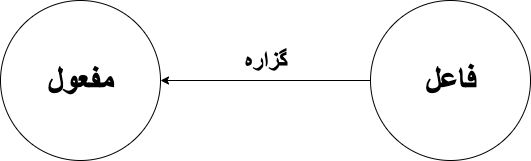
\includegraphics[scale=0.375]{figures/rdf/structure.png}
	\caption[ساختار انتزاعی گراف \lr{RDF}]{ساختار انتزاعی گراف \lr{RDF}}
	\label{fig:rdf-strcutre}
\end{figure}
	\columnbreak
\begin{figure}[H]
	\centering
	
\includegraphics[scale=0.375]{figures/rdf/sample.png}
	\caption[نمونه‌ای از یک سه‌تایی \lr{RDF}]{نمونه‌ای از یک سه‌تایی \lr{RDF}}
	\label{fig:rdf-sample}
\end{figure}
\end{multicols}

\section{سیستم پرسش و پاسخ}
سیستم‌ پرسش و پاسخ\footnote{\lr{Question Answering System}} به سیستمی گفته می‌شود که بتواند سوالات مطرح شده توسط یک انسان در زبان طبیعی را بررسی کرده و به آن به صورت خودکار پاسخ دهد. اینگونه سیستم‌ها در زمینه‌ی پردازش زبان طبیعی و بازیابی اطلاعات بررسی می‌شوند.\\
یک روش دسته‌بندی سیستم‌های پرسش و پاسخ مبتنی بر گراف دانش، بر اساس تعداد روابطی از گراف است که برای پاسخ‌دهی به سوال استفاده می‌شود. \\
دسته اول سوالات ساده هستند که برای پاسخ‌دهی به این سوالات فقط نیاز به یک رابطه از گراف دانش می‌باشد. به عنوان مثال در سوال "نام آثار سعدی چه هستند؟" با بررسی رابطه‌ی "آثار" از موجودیت "سعدی" در گراف دانش می‌توان پاسخ‌های این سوال را استخراج نمود. سیستمی که در این پروژه بررسی می‌شود از این دسته می‌باشد.\\دسته دوم سوالات پیچیده هستند که برای پاسخ دادن به آنها به بیش از یک رابطه از گراف دانش نیاز است. به عنوان مثال برای پاسخ دادن به سوال "علی دایی در کدام تیم‌های لیگ آلمان بازی کرده است؟" ابتدا باید رابطه‌ی "باشگاه" از موجودیت "علی دایی" بررسی شده و سپس رابطه‌ی "لیگ" روی هر کدام از نتایج رابطه‌ی اول بررسی شود.

\section{شبکه‌‌های عصبی}
در این قسمت به توضیح شبکه‌های عصبی و پایه‌ی ریاضی آنها و همچنین تشابه آنها با ریشه‌ی زیستی و طبیعی این شبکه‌ها پرداخته می‌شود. در ادامه نیز با انواعی از اینگونه شبکه‌ها آشنا خواهیم شد.
یکی از روش‌های نوین در یادگیری‌ ماشینی\footnote{\lr{Machine Learning}}، شبکه‌های عصبی یا به عبارتی شبکه‌های عصبی مصنوعی\footnote{\lr{Artificial Neural Networks}} بوده که می‌توان از آنها برای برای اعمال دانش بدست آمده از سامانه‌های پیچیده استفاده نمود. ساختار این شبکه‌ها مشابه ساختار زیستی مغز طبیعی بوده و از آن الهام گرفته است.
هسته‌ی اصلی پردازشی این شبکه‌ها نرون‌های مصنوعی‌‌\footnote{\lr{Artificial Neurons}} هستند که در شمار فراوان در این شبکه‌ها ظاهر شده و می‌توانند‌ به صورت کاملا به‌هم‌پیوسته\footnote{\lr{Fully Connected}} یا غیرکاملا به‌هم‌پیوسته\footnote{\lr{Not Fully Connected}} کنار هم قرار گیرند. در شبکه‌های طبیعی، ارتباطات کاملا به‌هم‌پیوسته بوده و در صورت آسیب دیدن یک نرون، نرون دیگری می‌تواند کار آن‌را به ‌عهده بگیرد. 
نرون‌های مصنوعی همانند گونه‌ی طبیعی خود قابلیت یادگیری دارند. یادگیری یک شبکه عصبی مصنوعی میتواند به صورت با نظارت\footnote{\lr{Supervised Learning}} و یا بدون نظارت\footnote{\lr{Unsupervised Learning}} انجام گیرد. شبکه‌هایی که در ادامه بررسی می‌شوند تحت روش یادگیری با نظارت آموزش می‌بینند.
\subsection{تعریف پایه}
یک شبکه‌ی عصبی دارای چندین لایه از نرون‌ها می‌باشد. عموما هر شبکه دارای سه لایه‌ی اصلی ورودی، پردازش و خروجی است. به طور معمول نرون‌های هر لایه به تمامی نرون‌های لایه‌های قبل و بعد خود متصل می‌شود مگر آنکه به طور مخصوص این ارتباط محدود گردد. در عین حال هیچ نرونی با نرون‌های هم‌لایه‌ی خود اتصالی برقرار نمی‌کند. نرون کوچکترین واحد پردازشگر در شبکه است و یک شبکه مجموعه‌ای از نرون‌ها می‌باشد که با معماری خاصی کنار هم قرار گرفته و متصل شده‌اند. رفتار یک شبکه حاصل از مجموع رفتار همگی نرون‌های آن شبکه است که به طور مستقل در حال پردازش می‌باشند. هر نرون می‌تواند یک تابع ریاضی خطی یا غیرخطی باشد. در نتیجه یک شبکه‌ی عصبی می‌تواند روابط ریاضی بسیار پیچیده‌ای را برای استفاده فراهم نماید.
\subsection{شبکه‌های عصبی پرسپترون و پرسپترون چندلایه}
پرسپترون ساده‌ترین نوع شبکه‌های عصبی است که یک دسته‌بند دو‌دویی\footnote{\lr{Binary Classifier}} به‌شمار می‌آید. فرض کنید که ورودی‌های شبکه‌ی عصبی $d$ بعدی بوده و به‌تعداد $n$ داده در اختیار داشته باشیم. در این صورت یک پرسپترون ورودی‌ خود $x \in R^{d}$ را به مقدار خروجی $f(x) \in R$ با رابطه‌ی زیر تبدیل می‌کند: 

\begin{equation}
\label{eqn:perceptron}
	f(x) = \begin{cases}
	1 & \ \ if \ <w, x> +\ b > 0 \\
	0 & \ \ otherwise
	\end{cases}
\end{equation}

که مقدار $w \in R^d$ بردار وزن  شبکه و $b$ نشان‌دهنده‌ی بایاس آن است که وظیفه‌ی آن جابجایی مرز تصمیم‌گیری از مبدا است. نماد $<w,x>$ نشان‌دهنده‌ی ضرب داخلی دو بردار است که مقدار آن برابر با $\sum_{i=1}^{m}w_i x_i$ می‌باشد.
طی مرحله‌ی یادگیری، شبکه‌ی پرسپترون تلاش می‌کند تا با توجه به داده‌هایی که در اختیار میگیرد، مقدار بهینه برای بردار وزنش یا همان $w$ و مقدار بایاسش یا همان $b$ را پیدا کند.
\subsubsection{پرسپترون‌ چند‌لایه}
یک پرسپترون چند‌لایه\footnote{\lr{Multi-Layer Perceptron}} شامل حداقل سه‌لایه ورودی، پردازش(پنهان) و خروجی می‌باشد. در واقع هر‌ شبکه‌ی عصبی با سه‌لایه یا بیشتر به یک پرسپترون چندلایه‌ نام‌گذاری می‌شود. برای مثال در شکل \ref{fig:perceptron} نمایشی از یک‌ شبکه‌ی پرسپترون با دو‌لایه‌ی پنهان آمده است. 
\begin{figure}[h]
	\centering
	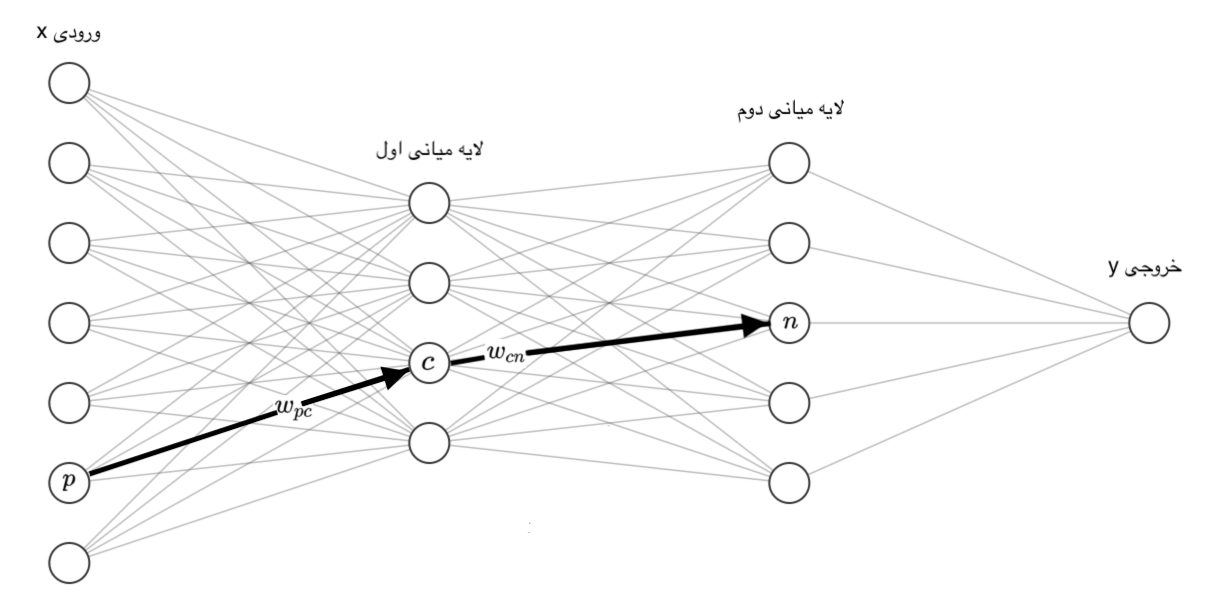
\includegraphics[scale=0.7]{figures/ml-perceptron.png}
	\caption[اتصالات یک شبکه‌ی عصبی پرسپترون با دو لایه‌ی پنهان]{اتصالات یک شبکه‌ی عصبی پرسپترون با دو لایه‌ی پنهان. گرادیان وزن‌های هر لایه وابسته به گرادیان وزن‌های لایه‌ی بالاتر می‌باشد.}
	\label{fig:perceptron}
\end{figure}
مقدار خروجی از نرون $p$ را با $b_p$ و وزن شبکه از نرون $p$ به $c$ را با $w_{pc}$ نمایش می‌دهیم. همانطور که در شکل \ref{fig:perceptron} مشخص است، نرون $c$ مقادیر تمامی نرون‌های لایه‌ی ورودی را دریافت کرده و روی آنها پردازش انجام می‌دهد. مجموع ضرب ورودی‌های نرون‌ $c$ با وزن‌هایشان را با $a_c$ نمایش می‌دهیم:
\begin{equation}
	a_c = \sum_{p}^{} w_{pc} b_{p}
\end{equation}
حال جهت ایجاد امکان مدل‌کردن روابط غیر‌خطی در ورودی‌ها، باید روی $a_c$ تابعی غیرخطی اعمال شود. در این صورت خواهیم داشت:
\begin{equation}
	b_c = \theta_c (a_c)
\end{equation}
که در آن $\theta_c$ تابع غیر‌خطی اعمال شده و $b_c$ خروجی جدید بدست‌آمده است. حال اگر تمامی‌ وزن‌های شبکه‌ی پرسپترون‌ را با $W$ نمایش دهیم و خروجی شبکه پرسپترون به ازای داده‌ی $x_i$ را $h_W(x_i)$ فرض کنیم، تابع هدف به‌صورت:
\begin{equation}
	Q(W) = \sum_{i = 1}^{n} l(h_W(x_i), y_i)
\end{equation}
خواهد بود که برای $l$ می‌توان از خطای‌ مربعات\footnote{\lr{Least Squared Error}} و یا منفی لگاریتم درست‌نمایی\footnote{\lr{Negative Log Likelihood}} استفاده کرد. 

برای بدست آوردن کمینه‌ی $Q(W)$ باید از روش گرادیان کاهشی\footnote{\lr{Gradient Descent}} استفاده کرد.  به این معنی که گرادیان تابع را حساب کرده، کمی در خلاف جهت آن حرکت کرده و این کار را آنقدر ادامه داد تا تابع هزینه خیلی کوچک شود. روش انتشار معکوس\footnote{\lr{Backpropagation}} در واقع روشی برای پیدا کردن گرادیان تابع $Q(W)$ نسبت به تمامی وزن‌های شبکه می‌باشد.

\subsection{شبکه‌ی عصبی پیچشی}
شبکه‌های پرسپترون چندلایه که در بخش قبل معرفی شدند با آنکه قابلیت یادگیری روی داده‌های غیرخطی را دارند اما در مسائلی با داده‌های حجیم مانند تصاویر دچار مشکل شده و با چنین ساختاری نیاز به تعداد پارامترهای زیادی دارند که موجب مشکل شدن فرایند یادگیری در اینگونه مسائل خواهد شد. برای رفع این مشکل از مفهوم و عملیات کانولوشن\footnote{\lr{Convolution}} استفاده شده و شبکه‌هایی با نام شبکه‌ی عصبی پیچشی\footnote{\lr{Convolutional Neural Network}} معرفی می‌شوند. عملیات پایه‌ای اینگونه شبکه‌ها عملیات کانولوشن می‌باشد. در این ساختار تعدادی هسته یا فیلتر وجود دارد که به آنها هسته‌ی لغزشی گفته می‌شود. این هسته‌ها همانند عملیات کانولوشن بر روی هر قسمت از داده‌ها قرار گرفته و پردازش انجام می‌دهند و این کار را روی همه‌ی قسمت‌های تصویر تکرار می‌کنند. هرکدام از این هسته‌ها دارای وزن‌هایی هستند که در مرحله‌ی یادگیری مورد آموزش قرار می‌گیرند. رابطه‌ی \ref{eqn:conv_rel} نشان دهنده‌ی این عملیات است. در این رابطه $x$ تصویر ورودی، $y$ ترم بایاس، $K$ اندازه‌ی هسته لغزشی،  $w$ وزن‌های آموزش (هسته‌ی لغزشی) و $z_{i, j}$ خروجی عملیات کانولوشن است. 
\begin{equation}
\label{eqn:conv_rel}
	Z_{i,j} = y_{i, j} + \sum_{m=0}^{K-1}\sum_{n=0}^{K-1}x_{i+m, j+n}w_{m,n}
\end{equation}

ترکیب این عملیات با اعمالی که در ادامه به آنها اشاره می‌کنیم،  شبکه‌ی عصبی با قابلیت بالا در پردازش تصاویر را نتیجه خواهد داد. این اعمال عبارتند از:
\begin{itemize}
	\item پولینگ\footnote{\lr{Pooling}}:
	عمل پولینگ یکی از اعمال اصلی شبکه‌های عصبی پیچشی بوده و به طور معمول  از آن استفاده می‌شود. از این عملیات برای کاهش بعد داده هنگام پردازش استفاده می‌شود. این عمل روی قسمت‌های مختلف داده قرار گرفته و داده‌های آن قسمت را یکی می‌کند. برای انجام آن روش‌های مختلفی وجود دارد که از انواع آن می‌توان به پولینگ بیشینه\footnote{\lr{Max Pooling}} و پولینگ میانگین\footnote{\lr{Average Pooling}} اشاره نمود. از مزیت‌های این عملیات بی‌اثر کردن شبکه عصبی پیچشی نسبت به تغییرات تصاویر نظیر حرکات انتقالی \footnote{\lr{Translation}}  می‌باشد.
	
	\item توابع فعال‌ساز غیر‌خطی\footnote{\lr{Non-Linear Activation Functions}}:
	 این توابع مختص شبکه‌های پیچشی نیستند و در شبکه‌های پرسپترون نیز از قابلیت غیر‌خطی‌ای که فراهم ‌می‌کنند استفاده می‌شود، هرچند کاربرد آنها در شبکه‌های عصبی پیچشی اهمیت بسیار بالایی پیدا می‌کند. از جمله مهمترین توابع فعال‌ساز غیر‌خطی مورد استفاده در شبکه‌های عصبی پیچشی می‌توان به تابع خطی رقیق شده\footnote{\lr{Rectified Linear Unit}} یا به‌طور اختصاری \lr{ReLU} اشاره داشت. ویژگی خاص این تابع که نمودار آن در \ref{fig:relu} نشان داده شده است در این است که در عین حال که غیرخطی بوده و می‌تواند یه یادگیری الگوهای پیچیده غیرخطی کمک کند، پردازش آن راحت بوده و مشتق آن بسیار ساده محاسبه می‌شود و استفاده از آن به‌صرفه‌تر از توابع غیرخطی‌ای نظیر تانژانت هایپربولیک\footnote{\lr{Tanh}} می‌باشد.
\end{itemize}

\begin{figure}[t!]
	\centering
	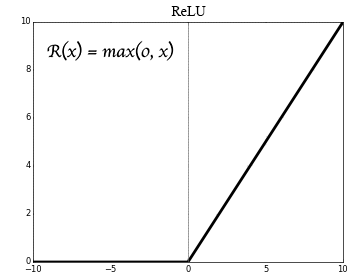
\includegraphics[scale=0.55]{figures/relu.png}
	\caption[نمودار تابع فعال‌ساز غیرخطی \lr{ReLU} مورد استفاده در شبکه‌های پیچشی]{نمودار تابع فعال‌ساز غیر‌خطی \lr{ReLU} مورد استفاده در شبکه‌های پیچشی‌}
	\label{fig:relu}
\end{figure}

\begin{figure}[t!]
	\centering
	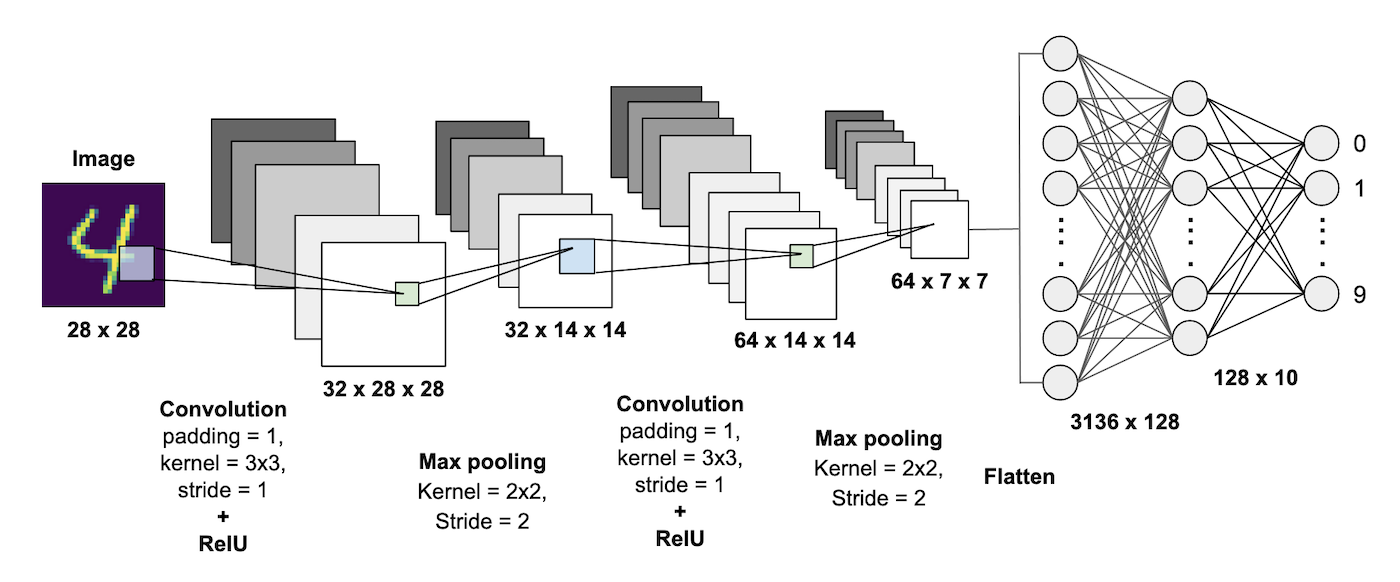
\includegraphics[scale=0.3]{figures/cnn-handwriting.png}
	\caption[معماری کلی یک شبکه‌ی عصبی پیچشی]{معماری کلی یک شبکه‌ی پیچشی در دسته‌بندی اعداد دست‌نوشته}
	\label{fig:cnn}
\end{figure}
نهایتا با ترکیب عملیات کانولوشن و پولینگ، و تکرار این امر در زمان آموزش، هسته‌های شبکه‌ی پیچشی مانند الگوریتم‌های مبتنی بر هسته‌های دست‌ساز در پردازش تصاویر یادگرفته و عمل می‌کنند. به عنوان مثال، در دسته‌بندی تصاویر چهره‌ی انسان، هسته‌هایی برای شناسایی رنگ مو، حالت ابرو و حالت بینی چهره شکل میگیرد. این ویژگی‌ها با اینکه به لطف عملیات پولینگ ابعاد پایینی دارند اما برای تشخیص چهره بسیار کاربردی بوده و استفاده می‌شوند. بنابراین در انتهای شبکه عصبی پیچشی از یک دسته‌بند مبتنی بر شبکه عصبی برای تشخیص خروجی استفاده می‌شود. نمونه‌ی چنین شبکه‌ای را که برای تشخیص اعداد دست‌نوشته استفاده می‌شود، در شکل \ref{fig:cnn} مشاهده می‌کنید. با توجه به وجود ۱۰ کلاس مختلف در مسئله‌ی تشخیص عدد دست‌نوشته، لایه‌ی دسته‌بند این شبکه که در انتهای آن قرار دارد دارای طول ۱۰ می‌باشد \cite{patel2019mnist}.
\subsection{شبکه‌‌ی عصبی بازگشتی}
ضعفی که در شبکه‌های معرفی شده در قسمت‌های قبل وجود دارد، ثابت بودن طول داده‌ی ورودی این شبکه‌ها می‌باشد.
در برخورد با داده‌های زبانی، صوت و یا فیلم، توالی و ترتیب اطلاعات اهمیت بالایی پیدا می‌کند. شبکه‌ی بازگشتی\footnote{\lr{Recurrent Neural Network}} این امکان را به ما می‌دهد تا یک توالی با طول نامشخص را به یک بردار با اندازه ثابت بازنمایی کنیم و در عین حال بسیاری از خواص نحوی و ساختاری توالی ورودی را حفظ کنیم. به طور کلی یک شبکه‌ی بازگشتی تابعی است که یک ورودی با طول غیرثابت (مثلا جمله) را به صورت دنباله‌ای از $n$ بردار با ابعاد $R^{d_{in}}$ دریافت و یک بردار خروجی $y$ با ابعاد $R^{d_{out}}$ باز می‌گرداند. رابطه‌ی زیر این موضوع را به‌خوبی بیان می‌کند:
\begin{equation}
\label{eqn:RNN}
	y_{n} = RNN(x_{1: n})
\end{equation}
که در آن $x_{1:n}$ جمله (دنباله) ورودی و $y_n$ بردار خروجی است. شکل \ref{fig:rnn} نمایشی از یک شبکه‌ی عصبی بازگشتی با سلول‌های حافظه‌ای ساده است. در واقع این شبکه از دو بخش اصلی تشکیل شده است:\\

\begin{enumerate}
	\item \textbf{بخش بازگشتی}:
	 این بخش با رابطه‌ی زیر نشان داده‌ می‌شود و به آن حالت درونی یا پنهان شبکه در زمان $t$ نیز گفته می‌شود:
	\begin{equation}
	\label{recursion}
		s_t = R(x_t, s_{t-1})
	\end{equation}
	\item \textbf{خروجی}:
	 که با اعمال تابع فعال‌ساز بر حالت بخش بازگشتی بدست می‌آید:
	\begin{equation}
	\label{output}
		o_t = O(s_t)
	\end{equation}
\end{enumerate}
به طور خلاصه، شبکه بازگشتی هر کلمه را به یک بردار $y_i$ تبدیل می‌کند ولی چون بردار مرحله آخر برگرفته از تمام اطلاعات قبلی است از آن به عنوان بازنمایی جمله استفاده می‌شود.
\begin{figure}[t!]
	\centering
	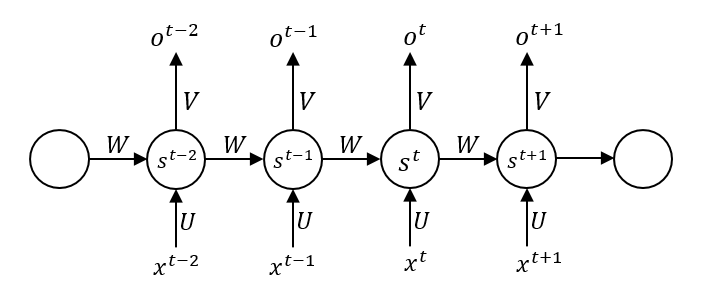
\includegraphics[scale=0.7]{figures/rnn.png}
	\caption[معماری کلی یک شبکه‌ی عصبی بازگشتی]{نمایی از معماری کلی یک شبکه‌ی عصبی بازگشتی متشکل از حالت‌های پنهان و خروجی‌ها}
	\label{fig:rnn}
\end{figure}

روابط \ref{recursion} و \ref{output} را به‌طور دقیق‌تر می‌توان اینگونه‌ بیان کرد:
\begin{equation}
s_t = tanh(Ws_{t-1} + Ux_{t-1})
\end{equation}
\begin{equation}
	o_t = y_t = softmax(Vs_t)
\end{equation}
واضح است که خروجی‌ زمان $t$ در یک شبکه‌ی عصبی بازگشتی به ورودی‌ها و حالت‌های پنهان زمان‌های قبلی وابسته است. به‌همین علت،‌ برای محاسبه‌ی گرادیان‌ها (تغییرات خطا نسبت به تغییر وزن‌ها) از الگوریتم انتشار معکوس در زمان\footnote{\lr{Backpropagation Through Time}} استفاده می‌شود. 

\subsection{شبکه‌ی عصبی دنباله به دنباله}
در شبکه بازگشتی بوسیله‌ی یک حلقه بر روی بردار ورودی جلو می‌رفتیم و هر بار یک خروجی ایجاد می‌کردیم. مشکلی که وجود دارد در مواقعی است که بایستی در سطح کل بردار پیش برویم تا شبکه به درستی آموزش ببیند. به طور مثال وقتی بخواهیم مفهوم یک جمله را برداشت کنیم تا انتهای آن باید پیش برویم، بنابراین تنها خروجی و یا وضعیت آخر برای ما مهم است. موردی که یک شبکه‌ی بازگشتی قادر به انجام آن نیست، تولید یک دنباله‌ از خروجی‌ها با توجه به تمامی اطلاعات ورودی می‌باشد. در چنین وضعیتی از یک شبکه‌ی عصبی دنباله به دنباله\footnote{\lr{Sequence to Sequence Neural Network}} استفاده می‌کنیم \cite{sutskever2014seq2seq}.
\subsubsection{ساختار شبکه}
یک شبکه‌ی دنباله به دنباله از ترکیب دو شبکه‌ی بازگشتی ساخته می‌شود. شبکه اول که کدگذار\footnote{\lr{Encoder}} نام دارد، دنباله‌ی بردار ورودی را به یک بردار وضعیت انتهایی تبدیل می‌کند و سپس آنرا به عنوان وضعیت اولیه برای شبکه بازگشتی دوم که کدگشا\footnote{\lr{Decoder}} نام دارد، در نظر می‌گیرد. شبکه‌ی کدگشا با هر گام که جلو می‌رود یک خروجی تولید می‌کند. بدین صورت دنباله‌ی خروجی مورد نظر ساخته می‌شود.
به عنوان مثال یک سیستم ترجمه‌کننده می‌تواند از این شبکه استفاده کند. به این صورت که ابتدا شبکه بازگشتی اول جمله زبان مبدأ را گرفته و آنرا به یک بردار وضعیت که نشان‌دهنده‌ی مفهوم جمله است، تبدیل می‌کند. سپس شبکه بازگشتی دوم این بردار وضعیت را دریافت کرده و جمله زبان مقصد را تولید می‌کند. در شکل \ref{fig:seq2seq} نمونه‌ای از این ماشین را مشاهده می‌کنید.

\begin{figure}[t!]
	\centering
	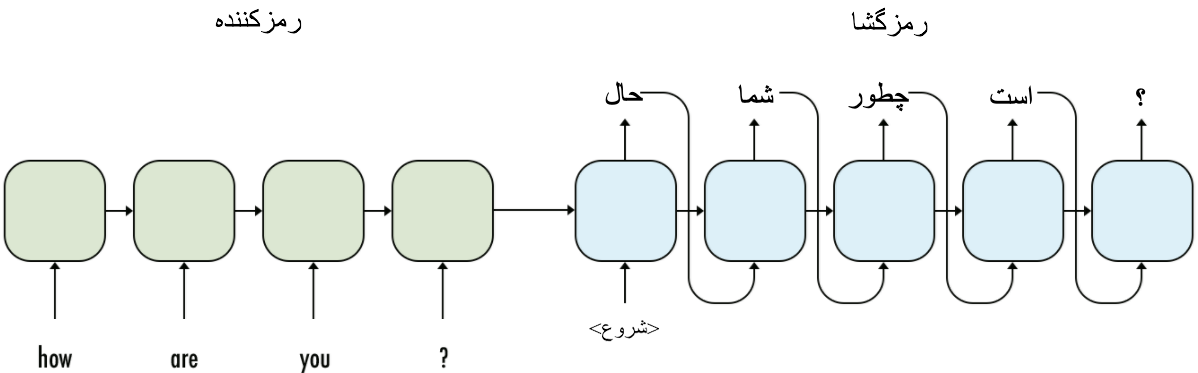
\includegraphics[scale=0.35]{figures/seq2seq.png}
	\caption[نمونه‌ای از شبکه‌ی دنباله به دنباله]{نمونه‌ی یک ماشین ترجمه که از شبکه‌ی دنباله به دنباله تشکیل شده است}
	\label{fig:seq2seq}
\end{figure}

\section{تابع هزینه‌ی \lr{Categorical Cross-Entropy}}
تابع \lr{Categorical Cross-Entropy} یک تابع هزینه\footnote{\lr{Loss Functoin}} مناسب برای دسته‌بندهای تک کلاسه\footnote{\lr{One-Class Classification}} است. دسته‌بندهای تک کلاسه دسته‌بندهایی هستند که هر داده‌ی آنها فقط متعلق به یک کلاس می‌باشد. این تابع هزینه به ازای هر داده بوسیله‌ی رابطه‌ی \ref{eqn:categorical_cross_entropy} بدست می‌آید که در آن $\hat{y}$ نماد بردار احتمالات پیشبینی شده توسط دسته‌بند و $y$ نماد بردار هدف می‌باشد.
\begin{equation}
\label{eqn:categorical_cross_entropy}
L(y, \hat{y}) = - \sum_{i = 0}^{n} (y_i * log(\hat{y}_i))
\end{equation}

\chapter{مروری بر کارهای گذشته}
از آنجا که سیستم‌های پرسش و پاسخ در تمامی زبان‌ها از اهمیت بالایی برخوردار هستند تحقیقات و پروژه‌های بسیاری با روش‌های متنوع برای پاسخ‌دهی به این مسئله ارائه شده است. در ادامه به بررسی تعدادی از روش‌های پیاده‌سازی شده که سعی در ارائه‌ی پاسخ و یا بهبود اینگونه سیستم‌ها را داشته‌اند می‌پردازیم. برخی از این روش‌ها برای پاسخ‌دهی به سوالات ساده و برخی برای سوالات پیچیده طراحی شده‌اند و همگی آنها مبتنی بر پایگاه دانش می‌باشند.

\section{روش‌های مبتنی بر ارائه‌ی معنایی}
در این روش‌ها تلاش می‌شود تا از سوال ورودی بازنمایی‌ای\footnote{\lr{Representation}} استخراج شود که حاوی معنای نهفته در سوال باشد تا بر اساس آن بتوان به کوئری متناسب با سوال رسید. در یکی از این روش‌ها از تجزیه‌کننده‌های\footnote{\lr{Parser}} موجود برای زبان انگلیسی استفاده می‌شود. هدف تولید یک کوئری الگو\footnote{\lr{Template}} متناسب با بازنمایی معنایی\footnote{\lr{Semantic}} تولید شده می‌باشد. منظور از کوئری الگو یک کوئری \lr{SPARQL} ناقص است که قالب آن کامل بوده اما بدون شناسه می‌باشد. یک کوئری الگو دارای جایگاه‌های مشخص برای قرار گرفتن شناسه‌های مرتبط با سوال می‌باشد. در این روش در تجزیه‌کننده‌ی مورد استفاده تغییراتی ایجاد شده که در حین تجزیه‌ی جمله بتواند کوئری الگو متناسب را تولید نماید. در مرحله‌ی بعدی موجودیت‌های جمله تشخیص داده شده و در جایگاه‌های مربوطه قرار می‌گیرند تا کوئری‌های نهایی تولید شوند. با امتیازدهی این کوئری‌ها برترین آنها انتخاب شده و استفاده می‌شود \cite{unger2012tembased}.
\\در روشی دیگر بدون استفاده از تجزیه‌کننده‌های موجود یک بازنمایی معنایی تولید می‌شود. بدین منظور برخلاف روش قبلی، ابتدا موجودیت‌های جمله تشخیص داده شده و استخراج می‌شوند. سپس به روش تکرارشونده\footnote{\lr{Iterative}} ارائه‌ی مورد نظر به صورت یک گراف تولید می‌شود. در هر تکرار این مرحله با توجه به گراف و اجزای جمله و موجودیت‌های تشخیص داده شده تعدادی عمل قابل انجام است که بوسیله‌ی آنها گره‌هایی به گراف اضافه می‌شوند. در نهایت با استفاده از این گراف یک کوئری تولید می‌شود \cite{sorokin2017endtoendweak}.
\section{روش‌های مبتنی بر تشخیص رابطه}
همانطور که در فصل پیشین توضیح داده شد، گراف‌های دانش مجموعه‌ای از موجودیت‌ها هستند که توسط روابطی بهم متصل شده‌اند. در بسیاری از سیستم‌های پرسش و پاسخ هدف سیستم تشخیص موجودیت و رابطه‌ی مورد نظر سوال می‌باشد تا بوسیله‌ی آن بتوان با ایجاد کوئری موجودیت پاسخ را دریافت نمود. در یکی از روش‌های موجود کل فرایند به چهار قسمت شامل تشخیص موجودیت، پیوند دادن موجودیت، تشخیص رابطه و دریافت پاسخ تقسیم شده است که قسمت تشخیص رابطه به صورت یک دسته‌بند عمل می‌کند. در چنین روشی هر کدام از مراحل مستقل از بقیه‌ی مراحل می‌توانند بررسی شوند. هر کدام از سه مرحله‌ی اول توسط روش‌های مبتنی بر شبکه عصبی و یا غیر شبکه عصبی مورد آزمایش قرار گرفته‌اند و نتایج نشان از عملکرد نزدیک این دو دسته روش‌ها در این مسائل می‌دهد. در مرحله‌ی آخر این روش، از روابط و موجودیت‌های کاندید استفاده می‌شود تا موجودیت پاسخ مورد نظر یافت شود. این روش تنها توانایی پاسخ دادن به سوالات ساده را دارد \cite{mohammed2018strongbaseline}.\\
در روشی مشابه نیز ابتدا روابط و موجودیت‌های کاندید استخراج می‌شوند، اما برای توانایی پاسخ دادن به سوالات پیچیده از همگی این روابط و موجودیت‌ها هم‌زمان استفاده می‌شود. بدین منظور این روش تلاش می‌کند مسیری در گراف دانشی که استفاده می‌کند پیدا کند که همگی روابط و موجودیت‌های استخراج شده از سوال در آن مسیر وجود داشته باشد. چنین مسیری گره‌های دیگری را نیز دربر می‌گیرد که همان پاسخ‌های کاندید برای سوال می‌باشند \cite{zafar2018formalquery}.\\
یکی از ایراد‌های وارد بر دو روش فوق در این است که به دلیل مستقل بودن مراحل تشخیص موجودیت و تشخیص رابطه امکان تشخیص اشتباه بالا می‌رود. به عنوان مثال برای کلماتی که چندین موجودیت مشابه به آن‌ها در گراف دانش یافت می‌شود، با توجه به رابطه‌ی مورد پرسش می‌توان موجودیت مناسب‌تر را تشخیص داد. به همین دلیل در روشی دیگر روابط، موجودیت‌ها و سایر گره‌های گراف دانش همگی تحت عنوان یک عنصر در نظر گرفته شده و سعی می‌شود عناصر مرتبط با پرسش تولید شده و یک مسیر صحیح در گراف دانش متناسب با پرسش مورد نظر یافت شود \cite{lan2019kbtopic}.
\section{روش‌های تولیدکننده‌ی جمله‌ی پاسخ}
در روش‌های معرفی شده در دو قسمت قبلی خروجی نهایی مدل‌ها یک موجودیت از پایگاه دانش است که به عنوان پاسخ به پرسش ورودی برگردانده می‌شود. اما در برخی روش‌ها به این پاسخ قناعت نشده و تلاش می‌شود یک جمله‌ی کامل به عنوان پاسخ بازگردانده شود. به عنوان مثال در پاسخ به پرسش "پایتخت ایران کجاست" به جای کلمه یا موجودیت "تهران"، جمله‌ی "پایتخت ایران تهران است" نمایش داده می‌شود.
برای پیاده‌سازی چنین سیستمی، در \cite{yini2016neuralgenerative} از یک شبکه‌ی دنباله به دنباله استفاده می‌شود. همانطور که مشخص است برخی از کلمات خروجی از پایگاه دانش استخراج می‌شوند و این شبکه نمی‌تواند به تنهایی تمامی جمله‌ی پاسخ را تولید نماید. کلمات خروجی را می‌توان به دو دسته‌ تقسیم نمود؛ کلمات پایگاه که از پایگاه دانش استخراج می‌شوند و کلمات مشترک که برای تکمیل جمله تولید می‌شوند و نیازی به پایگاه برای تولید آنها نمی‌باشد. برای استفاده هم‌زمان این شبکه و پایگاه دانش، تغییراتی در قسمت کدگشای شبکه‌ی دنباله به دنباله داده شده است. در این قسمت در هر گام علاوه بر کلمه‌ی خروجی یک احتمال نیز تولید می‌شود که نشان می‌دهد آیا این کلمه از کلمات مشترک یا از کلمات پایگاه می‌باشد. در صورتی که تشخیص داده شود که در این گام یک کلمه‌ی پایگاه بایستی تولید شود، از پایگاه دانش استفاده شده و بوسیله‌ی موجودیت‌های یافت شده در جمله‌ی ورودی موجودیت مربوطه به جمله‌ی خروجی استخراج می‌گردد.
\section{جمع‌بندی}
همانطور که در این فصل توضیح داده شد یکی از رویکردهای متداول در این حوزه استفاده از دسته‌بندها برای تشخیص رابطه می‌باشد. در این پژوهش نیز سیستمی با این رویکرد پیشنهاد داده می‌شود که در ادامه به معرفی آن می‌پردازیم.
\chapter{سیستم پیشنهادی برای پرسش و پاسخ فارسی}
در این فصل سیستمی مناسب برای پاسخ‌دهی به مسائل شرح داده شده در فصل یک معرفی می‌شود. برای چنین سیستمی نیاز به یک پایگاه دانش می‌باشد تا اطلاعات مورد نیاز سیستم را فراهم نماید. برای فراهم کردن این اطلاعات از گراف دانش فارس‌بیس استفاده می‌شود. در ابتدای این فصل به معرفی این گراف دانش پرداخته شده و سپس بخش‌های دیگر سیستم معرفی می‌شوند.
\section{گراف دانش فارس‌بیس}
پایگاه دانش فارس‌بیس اولین پایگاه دانش طراحی شده مخصوص زبان فارسی می‌باشد.
فارس‌بیس از مدل فراداده‌ای چارچوب توصیف منابع برای ذخیره‌ی دانش استفاده می‌کند. برای اتصال به این پایگاه دانش و دریافت موجودیت پاسخ از زبان \lr{SPARQL}\footnote{\lr{SPARQL Protocol and RDF Query Language}} استفاده می‌شود.
برخلاف پایگاه‌های دانش انگلیسی زبان همانند \lr{Wikidata} که افراد مختلف بسیاری در گسترش آن کمک می‌کنند، در مورد پایگاه‌های فارسی زبان چنین اجتماع گسترده‌ای وجود ندارد و نمی‌توان به آن اتکا نمود؛ به همین سبب برای تولید پایگاه دانش فارس‌بیس از داده‌های خام متنی داخل وب استفاده شده و از طریق خزش وب دانش‌های موجود در آنها استخراج می‌گردند.
دانش‌های استخراج شده به صورت ترکیب‌های سه‌تایی در پایگاه فارس‌بیس ذخیره می‌شوند. این ترکیب‌های سه‌تایی شامل فاعل، مفعول و رابطه‌ی بین آنها می‌باشد. به عنوان مثال با استخراج این دانش که مادرید پایتخت کشور اسپانیا می‌باشد، سه‌تایی «اسپانیا، مادرید، پایتخت یک کشور» در پایگاه دانش ایجاد می‌شود.
سیستم استخراج‌کننده‌ی دانش فارس‌بیس دارای معماری‌ای با چندین لایه می‌باشد. استخراج دانش از ترکیب دو روش اصلی استخراج رابطه\footnote{\lr{Relation Extraction}} و استخراج اطلاعات\footnote{\lr{Information Extraction}} صورت می‌گیرد. برای استخراج رابطه از دو ماژول و برای استخراج اطلاعات از چهار ماژول مختلف توسعه‌یافته برای زبان فارسی استفاده می‌شود. همچنین در هر دو روش یک مرحله‌ی پیوند موجودیت‌ها\footnote{\lr{Entity Linking}} وجود دارد که فاعل و مفعول سه‌تایی مربوطه را ابهام‌زدایی کرده و به موجودیت‌های گراف دانش متصل می‌نماید. به موازات این مرحله، کانونی‌‌سازی\footnote{\lr{Canonicalization}} نیز انجام می‌شود. در مرحله‌ی کانونی‌سازی رابطه‌ی بین فاعل و مفعول در اطلاعات استخراج شده بدست آورده می‌شود. این مرحله فقط در روش استخراج اطلاعات مورد نیاز است. در نهایت، همه‌ی سه‌تایی‌های دانش کاندید که استخراج شده‌اند، پس از بازبینی و تایید شدن توسط یک متخصص انسانی به پایگاه دانش فارس‌بیس افزوده می‌شوند \cite{farsbase}.
سیستم پرسش و پاسخ فارسی مورد نظر از این پایگاه دانش استفاده می‌کند تا با داشتن رابطه و موجودیت مورد پرسش، سه‌تایی مربوطه در پایگاه دانش را پیدا کرده و پاسخ سوال را از آن استخراج نماید. برای انجام این کار نیاز است که سه زیرمسئله‌ی عنوان شده در فصل یک شامل تشخیص رابطه، تشخیص موجودیت‌ها و تولید کوئری توسط سیستم پاسخ داده شوند. برای پاسخ دادن به این زیرمسئله‌ها نیاز به مجموعه دادگان وجود دارد و با توجه به نبود دادگان برای پرسش و پاسخ فارسی، دادگان مورد نیاز در این پروژه تهیه شده‌اند. در ادامه با دادگان جمع‌آوری شده آشنا شده و سپس به شرح چگونگی انجام و حل سه زیرمسئله‌ی عنوان شده که سه بخش اصلی سیستم را تشکیل می‌دهند، می‌پردازیم.
\section{مجموعه دادگان}
به تعداد ۴۶ رابطه از گراف دانش فارس‌بیس استخراج شده است که آنها را در جدول \ref{tab:relations} مشاهده می‌نمایید. این روابط جز پرکاربردترین روابط در گراف دانش می‌باشند که توسط تهیه‌کنندگان گراف دانش فارسی مشخص شده‌اند.
\begin{longtable}{|c|c|}
	\hline
	\rowcolor{headerColor} 
	عنوان & شناسه
	\\ \hline پایتخت یک کشور & \lr{http://fkg.iust.ac.ir/ontology/capital}
	\\  واحد پول یک شرکت & \lr{http://fkg.iust.ac.ir/ontology/currency}
	\\  نوع حکومت یک کشور & \lr{http://fkg.iust.ac.ir/ontology/governmentType}
	\\  زبان رسمی یک کشور & \lr{http://fkg.iust.ac.ir/ontology/language}
	\\  مساحت یک کشور & \lr{http://fkg.iust.ac.ir/ontology/areaTotal}
	\\  جمعیت یک کشور & \lr{http://fkg.iust.ac.ir/ontology/populationTotal}
	\\  کارگردان یک فیلم & \lr{http://fkg.iust.ac.ir/ontology/director}
	\\  بازیگران یک فیلم & \lr{http://fkg.iust.ac.ir/ontology/starring}
	\\  نویسنده یک فیلم & \lr{http://fkg.iust.ac.ir/ontology/writer}
	\\  آهنگساز یک فیلم & \lr{http://fkg.iust.ac.ir/ontology/musicComposer}
	\\  بودجه یک فیلم & \lr{http://fkg.iust.ac.ir/ontology/budget}
	\\  میزان فروش یک فیلم & \lr{http://fkg.iust.ac.ir/ontology/gross}
	\\  ترکیبات یک غذا & \lr{http://fkg.iust.ac.ir/ontology/ingredient}
	\\  آثار یک شخص & \lr{http://fkg.iust.ac.ir/ontology/notableWork}
	\\  باشگاه های یک ورزشکار & \lr{http://fkg.iust.ac.ir/ontology/club}
	\\  محل تحصیل یک شخص & \lr{http://fkg.iust.ac.ir/ontology/almaMater}
	\\  استاندار یک استان & \lr{http://fkg.iust.ac.ir/ontology/governorGeneral}
	\\  محل دفن یک شخص & \lr{http://fkg.iust.ac.ir/ontology/deathPlace}
	\\  تاریخ مرگ یک شخص & \lr{http://fkg.iust.ac.ir/ontology/deathDate}
	\\ فرزندان یک شخص & \lr{http://fkg.iust.ac.ir/ontology/child}
	\\  سرمربی یک تیم ورزشی & \lr{http://fkg.iust.ac.ir/ontology/property}
	\\  مرکز یک استان & \lr{http://fkg.iust.ac.ir/ontology/capital}
	\\  کارگردان یک سریال تلویزیونی & \lr{http://fkg.iust.ac.ir/ontology/director}
	\\  بازیگران یک سریال تلویزیونی & \lr{http://fkg.iust.ac.ir/ontology/starring}
	\\  نویسنده یک سریال تلویزیونی & \lr{http://fkg.iust.ac.ir/ontology/author}
	\\  قد یک ورزشکار & \lr{http://fkg.iust.ac.ir/ontology/Person/height}
	\\  مساحت یک دریا یا اقیانوس & \lr{http://fkg.iust.ac.ir/ontology/areaTotal}
	\\  دوره ساخت یک مکان یا بنا & \lr{http://fkg.iust.ac.ir/ontology/era}
	\\  همسر یک شخص & \lr{http://fkg.iust.ac.ir/ontology/spouse}
	\\  محل یک مکان یا بنا & \lr{http://fkg.iust.ac.ir/ontology/county}
	\\  ملیت یک شخص & \lr{http://fkg.iust.ac.ir/ontology/nationality}
	\\ نویسنده کتاب & \lr{http://fkg.iust.ac.ir/ontology/author}
	\\  ناشر کتاب & \lr{http://fkg.iust.ac.ir/ontology/publisher}
	\\  پیش شماره & \lr{http://fkg.iust.ac.ir/ontology/areaCode}
	\\  مساحت & \lr{http://fkg.iust.ac.ir/ontology/areaTotal}
	\\  جمعیت & \lr{http://fkg.iust.ac.ir/ontology/populationTotal}
	\\  شهردار & \lr{http://fkg.iust.ac.ir/ontology/leaderName}
	\\  محصولات شرکت & \lr{http://fkg.iust.ac.ir/ontology/service}
	\\  سایت یک شرکت & \lr{http://xmlns.com/foaf/0.1/homepage}
	\\ مدیر عامل شرکت & \lr{http://fkg.iust.ac.ir/ontology/ceo}
	\\  درامد & \lr{http://fkg.iust.ac.ir/ontology/revenue}
	\\  پلاک & \lr{http://fkg.iust.ac.ir/ontology/vehicleCode}
	\\  بزرگترین شهر یک کشور & بزرگترین\lr{\_}شهر\lr{http://fkg.iust.ac.ir/ontology/}
	\\  وزیر یک وزارتخانه & \lr{http://fkg.iust.ac.ir/ontology/leader}
	\\  تعداد کارکنان یک شرکت یا ارگان & \lr{http://fkg.iust.ac.ir/ontology/numberOfStaff}
	\\  نام ورزشگاه یک تیم ورزشی & \lr{http://fkg.iust.ac.ir/ontology/ground}
	\\ \hline	 	
	\caption{عنوان روابط و شناسه آنها در گراف دانش فارس‌بیس}
	\label{tab:relations}
\end{longtable}
\noindent به ازای هر کدام از روابط فوق مجموعه‌ای از جملات الگو به منظور آموزش به مدل‌ها در فایل \lr{rel\_q.csv} جمع‌آوری شده‌اند. تعدادی از الگوهای رابطه‌ی "پایتخت یک کشور" را در جدول \ref{tab:templates_capital} مشاهده می‌نمایید.
\begin{table}[h]
	\centering
	\def\arraystretch{1.6}
	\begin{tabular}{|c|}
		\hline
		پایتخت کشور ررر چه نام دارد
		\\پایتخت ررر چه نام دارد
		\\شهر ششش پایتخت کدام کشور است
		\\نام کشوری که شهر ششش پایتخت آن است چیست
		\\پایتخت کشور ررر چه می‌باشد
		\\ \hline	 
	\end{tabular}	
	\caption{نمونه‌هایی از جملات الگو برای رابطه‌ی "پایتخت یک کشور"}
	\label{tab:templates_capital}
\end{table}
\\در جملات الگو به جای موجودیت‌ها نماد آنها جایگزین شده است. به عنوان مثال در جملات جدول \ref{tab:templates_capital} "ررر" نماد موجودیت کشور و "ششش" نماد موجودیت شهر می‌باشد. هدف از انتخاب این نمادها اطمینان از عدم وجود آن‌ها در واژگان زبان فارسی می‌باشد. به ازای هر یک از این نمادها تعدادی موجودیت مرتبط از پایگاه دانش فارس‌بیس استخراج شده و در جملات الگو قرار داده می‌شوند و از این جملات تولید شده برای آموزش مدل‌ها استفاده می‌شود.

\section{تشخیص رابطه}
این بخش از سیستم وظیفه‌ی تشخیص رابطه‌ی موجود در سوال مورد پرسش کاربر را دارد که بوسیله‌ی یک دسته‌بند قابل انجام است. به این منظور دسته‌بندهای ماشین بردار پشتیبان و شبکه عصبی پیچشی که در فصل دوم با آن آشنا شدیم بکار گرفته شده‌اند. در این بخش به طور مختصر چگونگی استفاده از این دسته‌بندها برای این سیستم توضیح داده می‌شود. این دسته‌بندها در پکیج\footnote{\lr{Package}} \lr{classifiers} پیاده‌سازی شده‌اند. در این پکیج یک کلاس انتزاعی\footnote{\lr{Abstract}} پیاده شده و کلاس‌های مربوط به مدل‌های ماشین بردار پشتیبان و شبکه عصبی پیچشی از آن ارث‌بری می‌کنند. برای استفاده از این دسته‌بندها نیاز به یک مرحله پیش‌پردازش روی سوالات ورودی می‌باشد که در ادامه به شرح آن می‌پردازیم.

\subsection{‌تعبیه‌سازی کلمات}
برای استفاده از دسته‌بندها ابتدا باید سوالات ورودی به بردارهایی نگاشت شوند و از آن بردارها به عنوان ورودی دسته‌بند استفاده شود. برای این منظور از چهار روش تعبیه‌سازی\footnote{\lr{Embedding}} کلمات شامل کوله‌ی کلمات\footnote{\lr{Bag of Words}} که آنرا با نماد \lr{BOW} نمایش می‌دهیم، روش \lr{TF-IDF}\footnote{\lr{Term Frequency-Inverse Document Frequency}} و یک مدل \lr{word2vec} استفاده شده است. روش چهارم استفاده از همان مدل \lr{word2vec} به صورت وزن‌دار است که وزن‌های آن همان مقادیر معکوس فراوانی متن استفاده شده در روش \lr{TF-IDF} برای هر کلمه می‌باشد.
این مدل‌ها در فایل \lr{feature\_extractor.py} پیاده‌سازی شده‌اند. \\
مدل ماشین بردار پشتیبان با هر چهار روش فوق و مدل شبکه عصبی پیچشی با روش \lr{word2vec} بدون وزن قابل استفاده بوده و مورد آزمایش قرار گرفته‌اند.

\subsection{دسته‌بند ماشین بردار پشتیبان‌‌}
ماشین بردار پشتیبان یک روش یادگیری با نظارت است که از آن برای دسته‌بندی و رگرسیون\footnote{\lr{Regression}} می‌توان استفاده کرد. مبنای کار ماشین بردار پشتیبان دسته‌بندی خطی داده‌ها است به طوری که خطی به عنوان تقسیم‌کننده استفاده شود که بیشترین حاشیه اطمینان را داشته باشد. حل این مسئله منجر به یک مسئله‌ی بهینه‌سازی برنامه‌ریزی درجه دوم\footnote{\lr{Quadratic Programming}} مقید می‌گردد.
همچنین می‌توان از این ماشین برای دسته‌بندی داده‌های جدایی‌ناپذیر خطی هم استفاده کرد؛ به طوریکه قبل از استفاده از ماشین بردار پشتیبان، داده‌ها توسط تابعی تحت عنوان تابع هسته\footnote{\lr{Kernel}} به فضایی دیگر انتقال داده می‌شوند که در آن فضا جدایی‌پذیر خطی باشند. یک نمونه از این انتقال در شکل \ref{fig:svm-kernel} نمایش داده شده‌ است.\\
در این سیستم از تابع پایه شعاعی\footnote{\lr{Radial Basis Function (RBF)}} به عنوان هسته‌ی این دسته‌بند استفاده می‌شود.

\begin{figure}[t!]
	\centering
	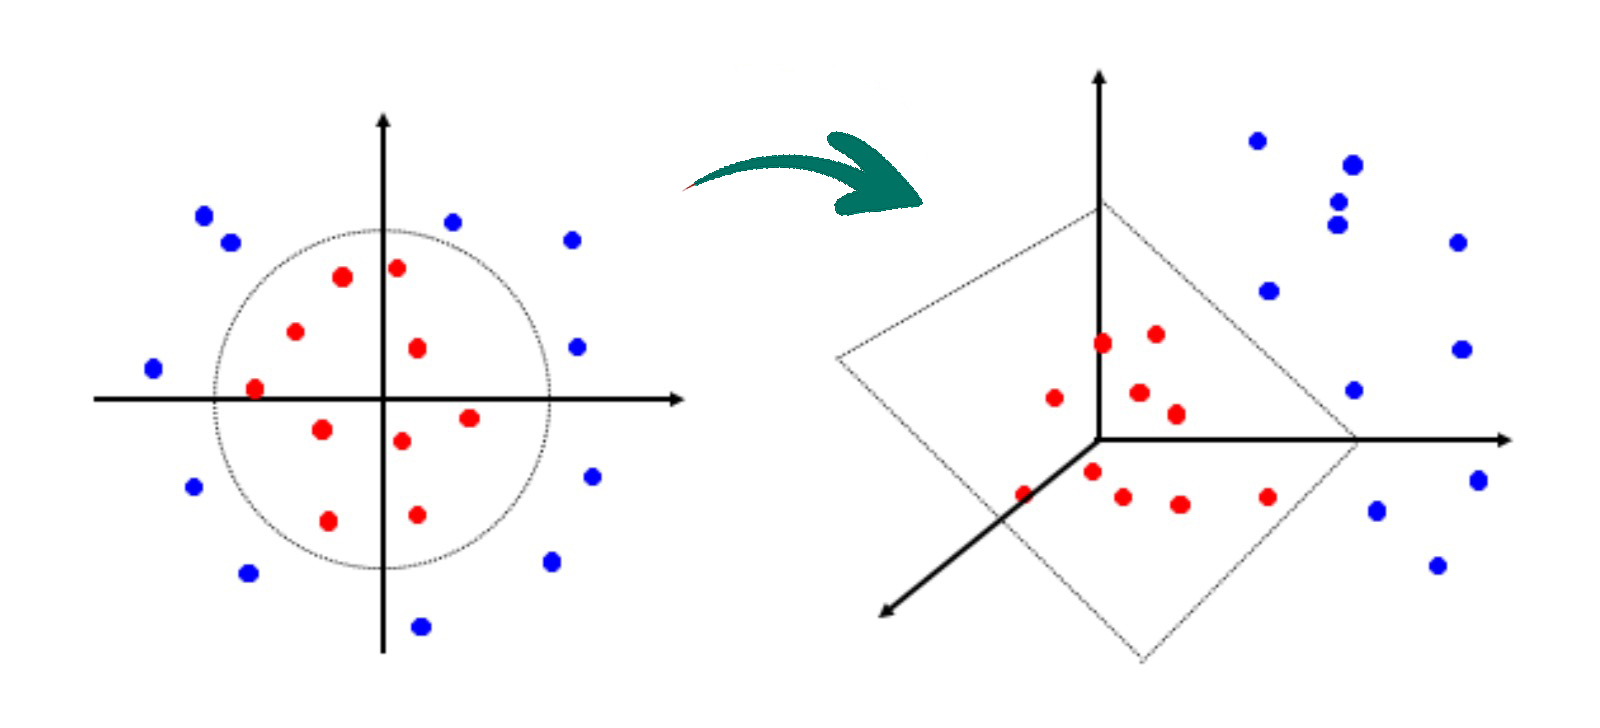
\includegraphics[scale=0.25]{figures/svm-kernel.jpeg}
	\caption[تابع هسته‌ی دایره‌ای در ماشین بردار پشتیبان]{جداپذیرخطی کردن داده‌ها با انتقالشان از فضای دوبعدی به سه‌بعدی بوسیله‌ی یک هسته‌ی تابع پایه شعاعی}
	\label{fig:svm-kernel}
\end{figure}

\subsection{دسته‌بند شبکه عصبی پیچشی}
پیاده‌سازی این شبکه توسط کتابخانه‌ی متن‌باز \lr{Keras} انجام شده است. این شبکه یک جمله را به صورت یک بردار تک‌بعدی دریافت می‌کند که هر خانه‌ی این آرایه کد کلمه‌ی متناطر در لیست واژگان را مشخص می‌کند. خروجی شبکه نیز یک بردار تک‌بعدی به طول ۴۶ می‌باشد که احتمال هر رابطه را برای جمله‌ی ورودی مشخص می‌نماید. همانطور که در شکل  \ref{fig:cnn-model} مشاهده می‌کنید، اولین لایه‌ی شبکه یک لایه‌ی تعبیه‌ساز است که از مدل \lr{word2vec} توضیح داده شده استفاده می‌کند تا هر کلمه را به بردار متناسب آن نگاشت کند.
لایه‌ی سوم که هسته‌ی این شبکه می‌باشد در ادامه توضیح داده خواهد شد. 
در ادامه دو لایه شبکه‌ از نورون‌ها (\lr{Dense}) همراه با تابع فعال‌ساز\footnote{\lr{Activation}} \lr{ReLU} حضور دارند که در نهایت بوسیله‌ی یک لایه‌ی فعال‌ساز \lr{Softmax} احتمالات هر یک از کلاس‌ها که خروجی دسته‌بند است تولید می‌شود. در میان این لایه‌ها دو لایه‌ی حذفی تصادفی\footnote{\lr{Dropout}} حضور دارند که فقط هنگام آموزش فعال هستند و هدف آنها کاهش بیش‌بردازش\footnote{\lr{Overfitting}} در هنگام آموزش می‌باشد. \\
هسته‌ی این شبکه، یک شبکه‌ی پیچشی است که وظیفه‌ی آن تشخیص الگوهای جملات ورودی است. همانطور که در شکل \ref{fig:cnn-model-core} مشاهده می‌کنید، این شبکه از سه قسمت موازی مشابه تشکیل می‌شود. در هر قسمت ابتدا یک لایه شبکه‌ی کانولوشن وجود دارد که در هر کدام از آنها ظرفیت لازم برای تشخیص ۱۵۰ فیلتر در نظر گرفته شده است. اما اندازه‌ی هسته یا فیلتر آنها متفاوت بوده و طول آن در هر کدام به ترتیب سه، چهار و پنج کلمه در نظر گرفته شده است. در ادامه در هر سه قسمت مقادیر به یک لایه‌ی ادغام حداکثر\footnote{\lr{Max Pooling}} به طول دو وارد شده و سپس تمامی مقادیر بهم الحاق شده و از این شبکه‌ی داخلی خارج می‌شوند \cite{yoon2014conv}.
\\از تابع هزینه‌ی \lr{Categorical Cross-Entropy} برای آموزش این شبکه استفاده شده است.
\begin{figure}
	\centering
	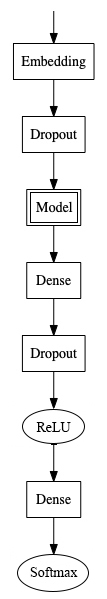
\includegraphics[width=3cm]{figures/cnn/cnn-model.jpg}
	\caption[لایه‌های دسته‌بند شبکه عصبی پیچشی]{لایه‌های دسته‌بند شبکه عصبی پیچشی}
	\label{fig:cnn-model}
\end{figure}

\begin{figure}
	\centering
	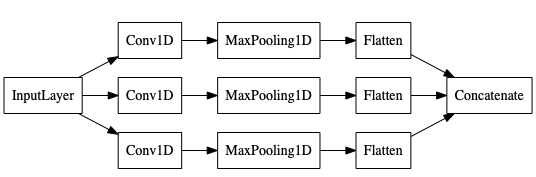
\includegraphics[width=15cm]{figures/cnn/cnn-model-core.jpg}
		\caption[لایه‌های هسته‌ی دسته‌بند شبکه عصبی پیچشی]{لایه‌های هسته‌ی دسته‌بند شبکه عصبی پیچشی}
	\label{fig:cnn-model-core}
\end{figure}

\section{تشخیص موجودیت‌ها}
برای تشخیص موجودیت‌های جمله‌ی مورد پرسش دو امکان در این سیستم موجود است. امکان اول استفاده از رابط‌های برنامه‌نویسی کاربردی\footnote{\lr{API}} موجود در سیستم فارس‌بیس است که امکان تشخیص موجودیت‌های موجود در جمله را دارند. امکان دوم استفاده از کتابخانه‌ی تشخیص‌دهنده موجودیت‌های نام‌دار\footnote{\lr{Named-Entity Recognition}} پیاده‌سازی شده در آزمایشگاه پردازش زبان طبیعی امیرکبیر است که در پکیج \lr{NER\_module} موجودند. 
در این سیستم خروجی هر دو روش گرفته شده و از آنهایی که گره‌ی مرتبط در گراف فارس‌بیس دارند استفاده می‌شود. روندهای مربوط به این قسمت در فایل \lr{NER\_provider} قابل مشاهده می‌باشند.
در ادامه خروجی این دو روش را برای جمله‌ی "پایتخت کشور آلمان کجاست" مشاهده می‌کنید. خروجی اول مربوط به رابط برنامه‌نویسی فارس‌بیس و خروجی دوم مربوط به کتابخانه‌ی تشخیص‌دهنده می‌باشد:
\begin{flushleft}
\lr{['Beginning :Thing', 'Beginning :Country', 'Inside :Country', 'Outside']}\\
\lr{['o', 'o', 'b-loc', 'o'].}
\end{flushleft}
\section{تولید کوئری}
رابطه و موجودیت‌ تشخیص داده شده توسط بخش‌های دیگر سیستم که توضیح داده شدند، در این بخش استفاده شده و کوئری مناسب تولید می‌شود. از آنجا که پایگاه دانش از یک گراف جهت‌دار ساخته شده است، موجودیت سوال می‌تواند در ابتدا و یا انتهای رابطه باشد. بر همین اساس کوئری ارسالی به دو صورت می‌تواند ساخته شود که هر دو قالب را در ادامه مشاهده می‌کنید:

\begin{multicols}{2}
	\begin{LTR}
		\begin{verbatim}
		select distinct(?o) where {
		<‌entity_uri> <relatoin_uri> ?o.
		}
		\end{verbatim}
	\end{LTR}
	\columnbreak
	
	\begin{LTR}
		\begin{verbatim}
		select distinct(?o) where {
		?o <relation_uri> <entity_uri>.
		}
		\end{verbatim}
	\end{LTR}
\end{multicols}
به عنوان مثال برای پرسش "پایتخت آلمان کجاست" موجودیت "آلمان" و رابطه‌ی "پایتخت یک کشور" بدست آورده شده‌اند. با استفاده از این اطلاعات و بدست آوردن جهت رابطه در این سوال کوئری زیر تولید می‌شود:
\begin{LTR}
	\noindent \lr{select distinct(?o) where }$\{$
	\\\lr{<http://fkg.iust.ac.ir/resource/}آلمان\lr{>}
	\lr{<http://fkg.iust.ac.ir/ontology/capital>}
	\lr{?o.}
	\\$\}$
\end{LTR}
اگر برای پرسش ورودی چندین رابطه با احتمال بالا و یا چندین موجودیت تشخیص داده شود، از ترکیب آنها چندین کوئری ساخته شده و در مرحله‌ی ارسال از همه‌ی آنها استفاده می‌شود و چندین پاسخ برای کاربر بازگردانده می‌شود. 

\chapter{تحلیل، طراحی و پیاده‌سازی سیستم}
در این فصل به توضیحات مربوط به تحلیل، طراحی و پیاده‌سازی سیستم پرداخته می‌شود. ابتدا متدولوژی مورد استفاده در این سیستم توضیح داده شده و سپس نیازمندی‌های سیستم بررسی می‌شوند. در ادامه با معماری این سیستم و بخش‌های مختلف آن آشنا شده و چگونگی پیاده‌سازی هر یک از بخش‌های سیستم جداگانه توضیح داده می‌شود.

\section{الگوی سیستم}
یک متدولوژی مجموعه‌ای از روش‌ها، توصیه‌ها و قالب‌ها است که به همراه راهبرد مشخص و طی مراحل مختلف، در توسعه‌ی سیستم به‌کار گرفته می‌شود. براساس رویکرد‌های مختلف متدولوژی‌های مختلفی وجود دارد. به‌عنوان مثال در رویکرد توسعه چابک\footnote{\lr{Agile}}، متدولوژی‌های اسکرام\footnote{\lr{Scrum}} و کانبان\footnote{\lr{Kanban}} وجود دارند. یا در رویکرد شیءگرا\footnote{\lr{Object Oriented}} متدولوژی \lr{RUP}\footnote{\lr{Rational Unified Process}} تعریف شده است. انتخاب متدولوژی وابسته به عوامل بسیاری چون نیازمندی‌های نرم‌افزار، تعداد اعضاء تیم، زمان‌بندی پروژه و ... می‌باشد. 
از آنجا که نیازمندی‌های سیستم به طور دقیق در ابتدا مشخص نبوده‌اند از الگوی چابک\footnote{\lr{Agile}} استفاده شده است. این الگو در واقع همان الگوی آبشاری\footnote{\lr{Waterfall Model}} است که در چندین تناوب تکرار می‌شود و ‌مراحل پیاده‌سازی و آزمایش همزمان با مراحل تحلیل و طراحی سیستم مورد نظر انجام می‌گیرد. در این الگو هر آنچه تولید می‌شود بلافاصله مورد آزمایش قرار می‌گیرد و سپس با تحلیل دوباره‌ی نیازمندی‌ها مراحل تکرار می‌شوند \cite{pressman2019software}. در الگوی چابک استفاده شده در این پروژه، مراحل زیر به ترتیب و به صورت تکرارشونده انجام شده‌اند:
\begin{enumerate}
	\item تحلیل نیازمندی‌ها
	\item برنامه‌ریزی
	\item طراحی سیستم
	\item پیاده‌سازی
	\item آزمایش‌
\end{enumerate}

در ادامه توضیحات مربوط به تحلیل، طراحی و پیاده‌سازی نرم‌افزار آورده شده‌ است. توضیحات مربوط به آزمایش و اعتبارسنجی قسمت‌های مختلف سیستم در فصل‌های مربوط به خودشان توضیح داده خواهد شد.

\section{تحلیل نیازمندی‌های سیستم}

این سیستم دو دسته استفاده کننده دارد.
دسته‌ی اول کاربر عادی سیستم است که نیازمندی‌های آن به شرح زیر است:

\begin{itemize}
	\item ورود سوال: کاربر عادی باید بتواند یک جمله را به عنوان پرسش مورد نظرش در سیستم ثبت کند تا سیستم آنرا بررسی کند.
	\item دریافت پاسخ: کاربر عادی باید بتواند پاسخ‌هایی که سیستم بدست آورده را مشاهده نماید.
	\item دریافت پاسخ‌های غیرمنتخب: این کاربر باید بتواند پاسخ‌های غیرمنتخب تشخیص داده شده توسط سیستم را مشاهده کند. این نیازمندی زیرمجموعه‌ی نیازمندی دریافت پاسخ می‌باشد. 
\end{itemize}
دسته‌ی دوم کاربر تحلیل‌گر است. تحلیل‌گر تمامی نیازمندی‌های ذکر شده برای کاربر عادی را شامل شده و نیازمندی‌های زیر را نیز دارد:

\begin{itemize}
	\item احراز هویت: تحلیل‌گر باید بتواند خود را به سیستم بشناساند و تحت عنوان تحلیل‌گربه سیستم ورود یا خروج کند. 
	\item دریافت اطلاعات میانی: تحلیل‌گر می‌تواند اطلاعات میانی سیستم که شامل کوئری‌های ارسال شده توسط سیستم است را مشاهده نماید.
\end{itemize}
نیازمندی‌های کاربردی سیستم توسط نمودار \lr{Use case} نمایش داده می‌شود. در شکل \ref{fig:use_case} این نمودار را مشاهده می‌کنید. همانطور که گفته شد این سیستم دارای دو نقش کاربر عادی و تحلیل‌گر می‌باشد.

\begin{figure}[t!]
	\centering
	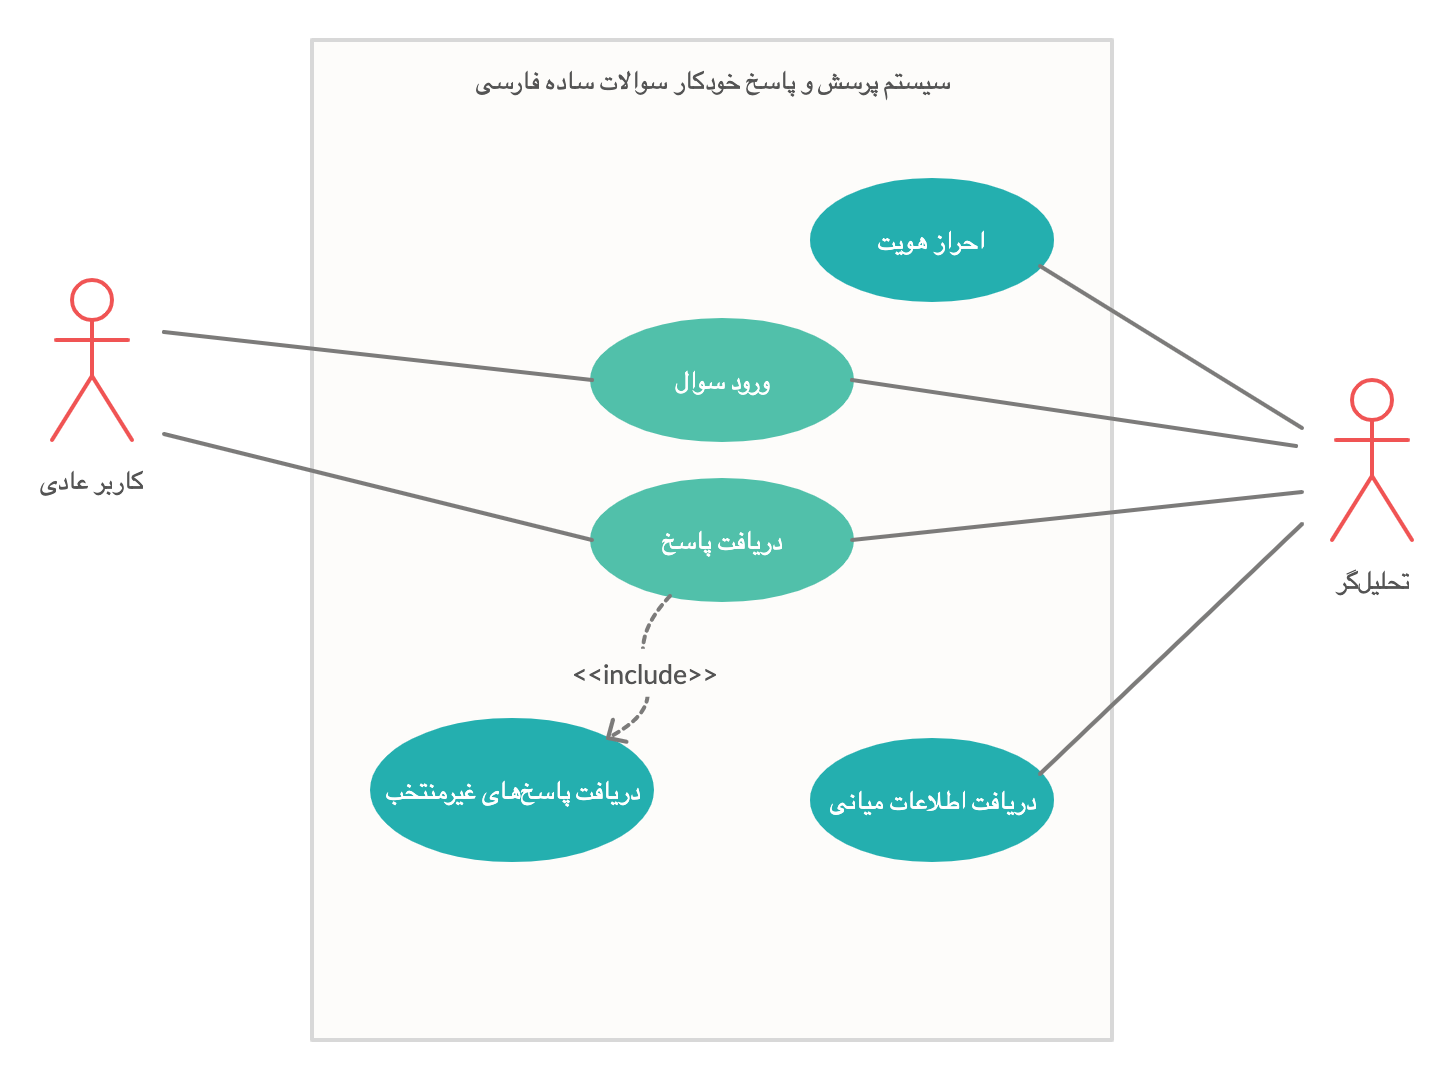
\includegraphics[width=15cm]{figures/se-diagrams/use-case.png}
	\caption[نمودار \lr{Use case}]{نمودار \lr{Use case}}
	\label{fig:use_case}
\end{figure}

\section{طراحی سیستم}
در شکل \ref{fig:architecture}  معماری این سیستم را مشاهده می‌کنید که از الگوی سرویس‌دهنده-سرویس‌گیرنده برای طراحی آن استفاده شده است.
این سیستم بوسیله‌ی یک رابط کاربری تحت وب برای کاربر ارائه می‌شود. بنابراین بخش‌های اصلی سیستم شامل بخش سرویس‌دهنده و سرویس‌گیرنده می‌باشد.
بخش سرویس‌دهنده دارای سه بخش اصلی هسته سیستم، سرویس وب و اتصال به پایگاه دانش می‌باشد. هسته سیستم بخش اصلی سیستم است و شامل مدل‌های یادگیری ماشین برای تشخیص رابطه و موجودیت‌های داخل سوال بوده و وظیفه‌ی تولید کوئری مرتبط را نیز دارد. بخش اتصال به پایگاه داده وظیفه‌ی ارسال کوئری و گرفتن پاسخ از گراف دانش را انجام می‌دهد. 
کاربر بوسیله‌ی رابط کاربری تحت وب با سرویس‌گیرنده و سرویس‌گیرنده بوسیله‌ی سرویس وب با سرویس‌دهنده در ارتباط است.

\begin{figure}[t!]
	\centering
	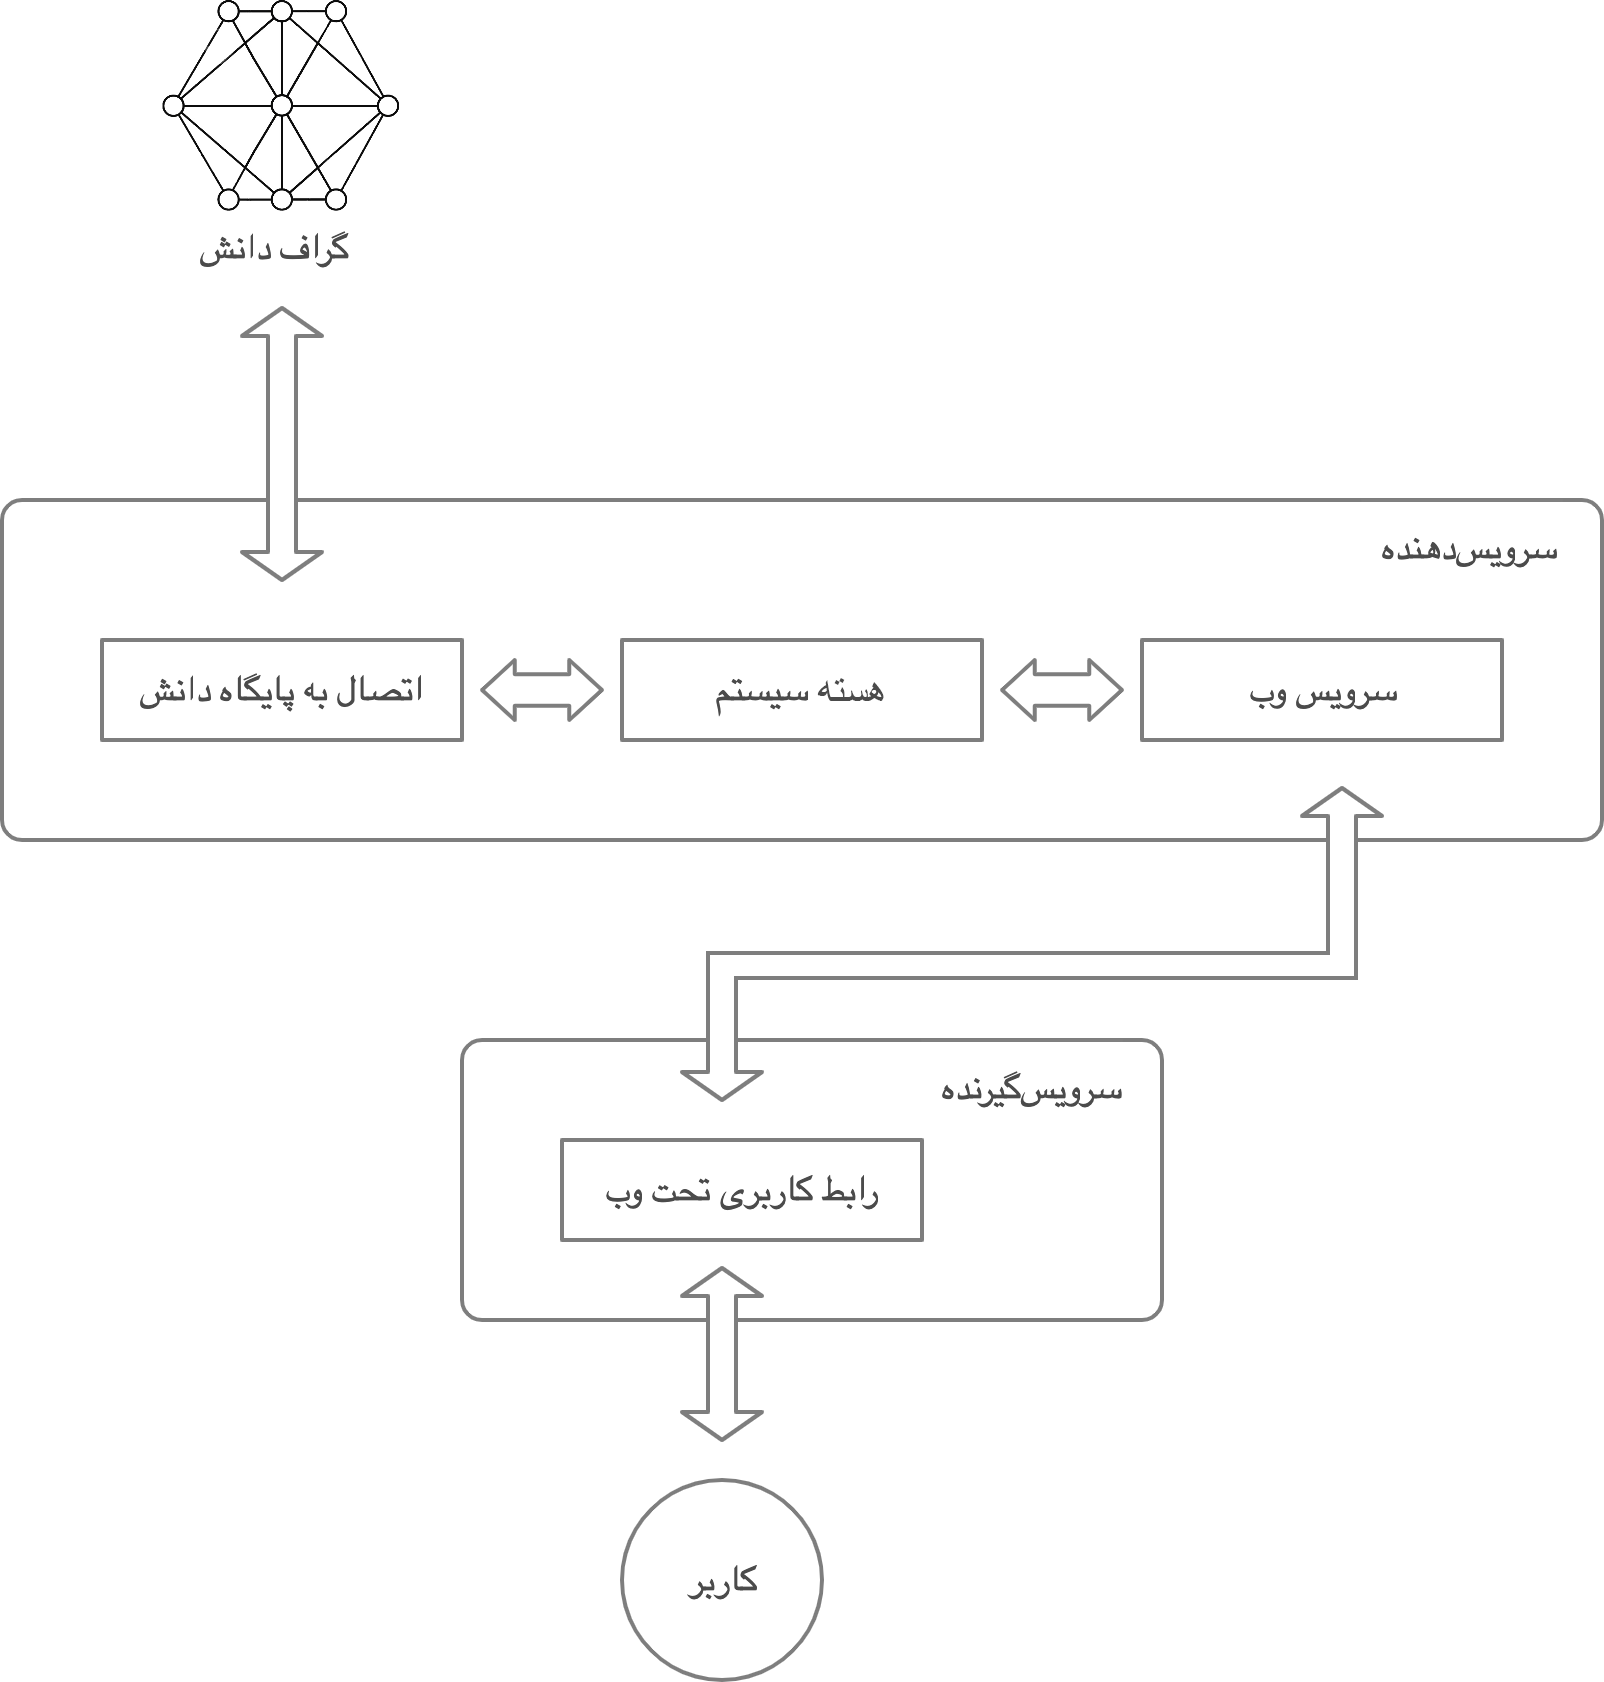
\includegraphics[width=12cm]{figures/se-diagrams/architecture.png}
	\caption[معماری سیستم]{معماری سیستم}
	\label{fig:architecture}
\end{figure}


\section{پیاده‌سازی سیستم}

بخش عمده‌ی این سیستم بوسیله‌ی زبان پایتون\footnote{\lr{Python}} نسخه‌ی ۳.۶.۷ پیاده‌سازی شده است. در این بخش هر کدام از قسمت‌های سیستم که در بخش طراحی ذکر شده‌اند توضیح داده خواهند شد.

\subsection{هسته سیستم}
هسته سیستم بخش اصلی این سیستم است که وظیفه‌ی آن پاسخ‌دهی به سه زیرمسئله‌ی اصلی سیستم شامل تشخیص رابطه، تشخیص موجودیت و تولید کوئری می‌باشد. این بخش همان سیستم پیشنهادی توضیح داده شده در فصل پیشین است.
فایل اصلی این قسمت \lr{answer\_generator.py} است که وظیفه‌ی آن آماده‌سازی روند پاسخ‌دهنده‌ی سوالات کاربران می‌باشد. در این فایل روندهای مورد نیاز برای سه زیرمسئله‌ی بیان شده فراخوانی شده و استفاده می‌شوند.
\subsection{اتصال به پایگاه دانش}
در فصل قبل چگونگی تولید کوئری مورد نیاز برای ارسال به پایگاه دانش فارس‌بیس شرح داده شد. بخش اتصال به پایگاه دانش وظیفه دارد که کوئری‌های تولید شده توسط سیستم را به پایگاه دانش ارسال کرده و پاسخ مرتبط را از پایگاه دریافت نموده و به سیستم بازگرداند. پایگاه دانش فارس‌بیس چنین درخواست‌هایی را از طریق آدرس \lr{http://farsbase.net:8890/sparql} پاسخ می‌دهد. این درخواست‌ها با استفاده از متد \lr{Post} در پروتکل \lr{HTTP} ارسال می‌شوند. پاسخ دریافتی از پایگاه دانش که به صورت \lr{XML} است می‌تواند در برگیرنده‌ی چندین موجودیت به عنوان پاسخ باشد. این موجودیت‌ها می‌توانند دارای گره در پایگاه دانش باشند که در این صورت آدرس آنها در پایگاه بازگردانده می‌شود.
روندهای مربوط به این قسمت در فایل \lr{graph\_extractor.py} پیاده‌سازی شده‌اند.
\subsection{سرویس و رابط کاربری تحت وب}
تمامی فایل‌های مربوط به این دو بخش از سیستم در پکیج \lr{web\_interface} قرار دارند.
\subsubsection{سرویس}
برای اتصال هسته سیستم به رابط کاربری وب از کتابخانه‌ی \lr{Flask} در پایتون استفاده شده است. بوسیله‌ی این کتابخانه رابطهای برنامه‌نویسی کاربردی مورد نیاز فراهم شده و بوسیله‌ی آنها روندهای متناسب در هسته سیستم فراخوانی می‌شوند.\\
دو مسیر\footnote{\lr{Route}} در این سرویس ارائه می‌شود. مسیر اول به آدرس \lr{"/"} صفحه‌ی اصلی رابط کاربری را برای کاربر نمایش می‌دهد که کاربر می‌تواند در این صفحه پرسش مورد نظر خود را وارد کرده و پاسخ را مشاهده کند. مسیر دوم به آدرس \lr{"/answer"} می‌تواند بوسیله‌ی متد\footnote{\lr{Method}} \lr{Post} در پروتکل \lr{HTTP} فراخوانی شود. این مسیر پرسش وارد شده توسط کاربر را همراه با پارامترهای دیگر دریافت کرده و با فراخوانی روند مورد نیاز در هسته سیستم پاسخ را در فرمت \lr{JSON} برمی‌گرداند.\\
این سرویس در فایل \lr{interface.py} پیاده‌سازی شده است.
\subsubsection{رابط کاربری}
در رابط کاربری کاربران می‌توانند پرسش خود را وارد کنند و رابطه و موجودیت تشخیص داده شده برای آن و پاسخ خود را دریافت نمایند. رابط کاربری تحت وب با فراخوانی رابطهای برنامه‌نویسی کاربردی پیاده‌سازی شده در سرویس وب با سرویس‌دهنده ارتباط برقرار می‌کند. برای کاربران این گزینه وجود دارد که اگر بخواهند سیستم روابط غیر منتخب را نیز برایشان بررسی کند که در این صورت احتمال درستی هر کدام از روابط تشخیص‌ داده شده نیز نمایش داده می‌شود. کاربر تحلیل‌گر می‌تواند اطلاعات میانی سیستم که شامل کوئری ارسالی می‌شود را نیز مشاهده کند. تصاویری از رابط کاربری را همراه با پرسش‌ها و حالات مختلف مشاهده می‌کنید.
\vfill
\begin{figure}[h]
	\centering
	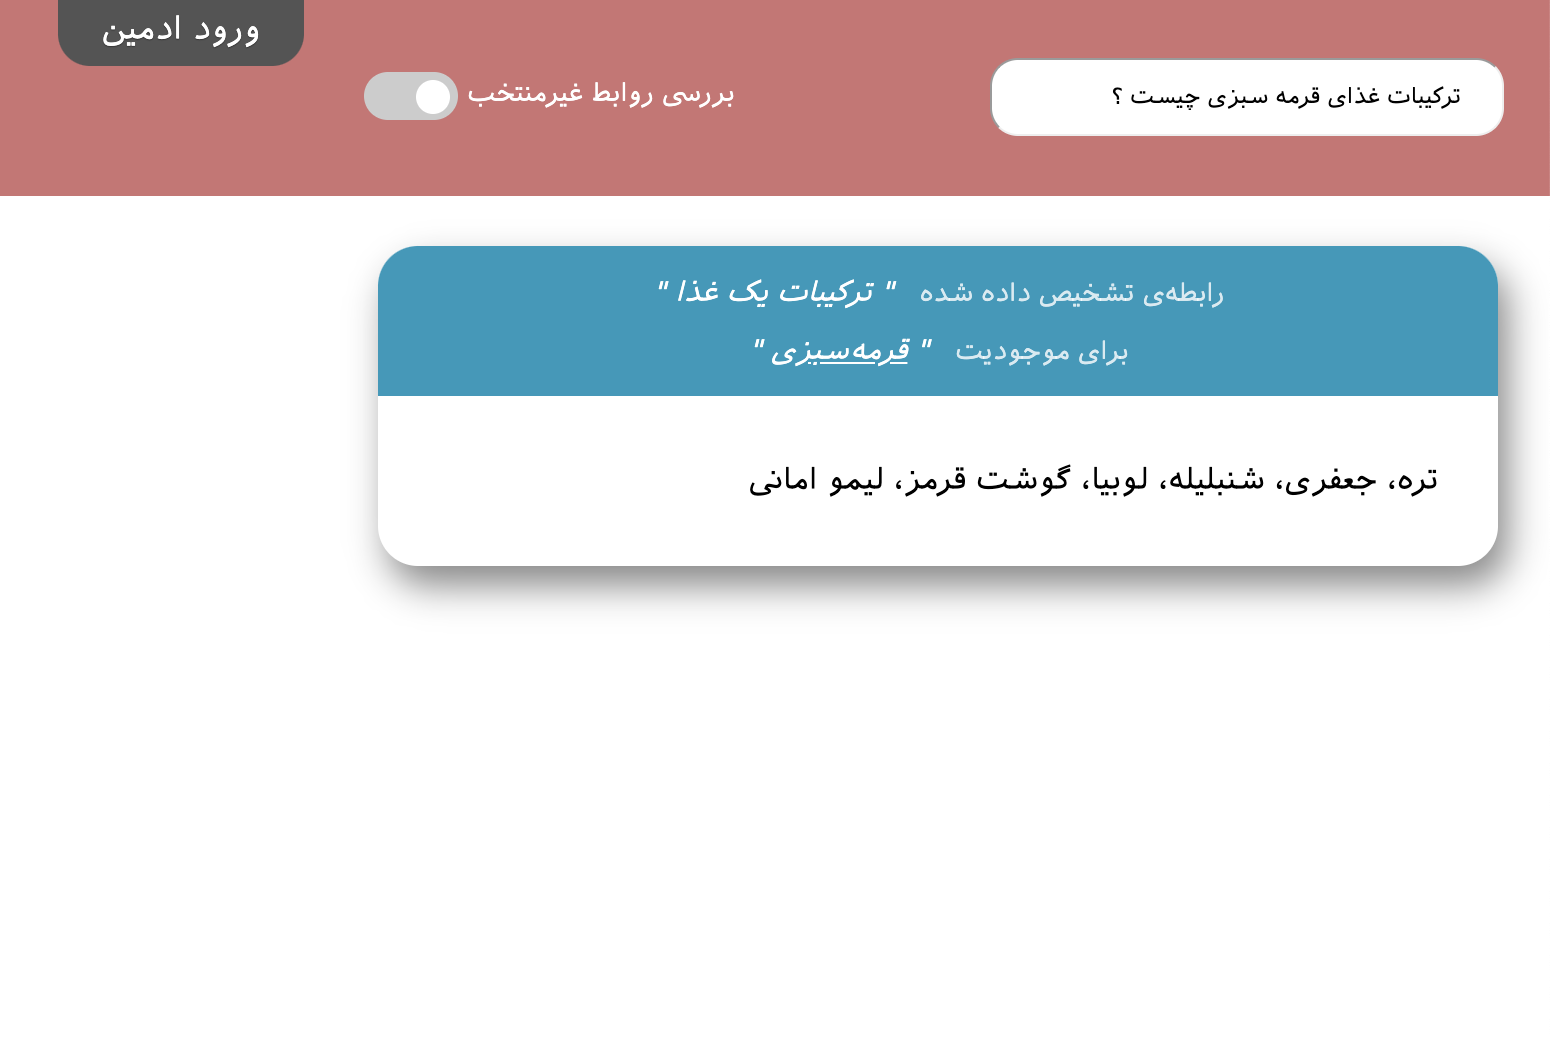
\includegraphics[width=15cm]{figures/interface/user.png}
	\caption{صفحه کاربر عادی}
\end{figure}
\vfill
\begin{figure}
	\centering
	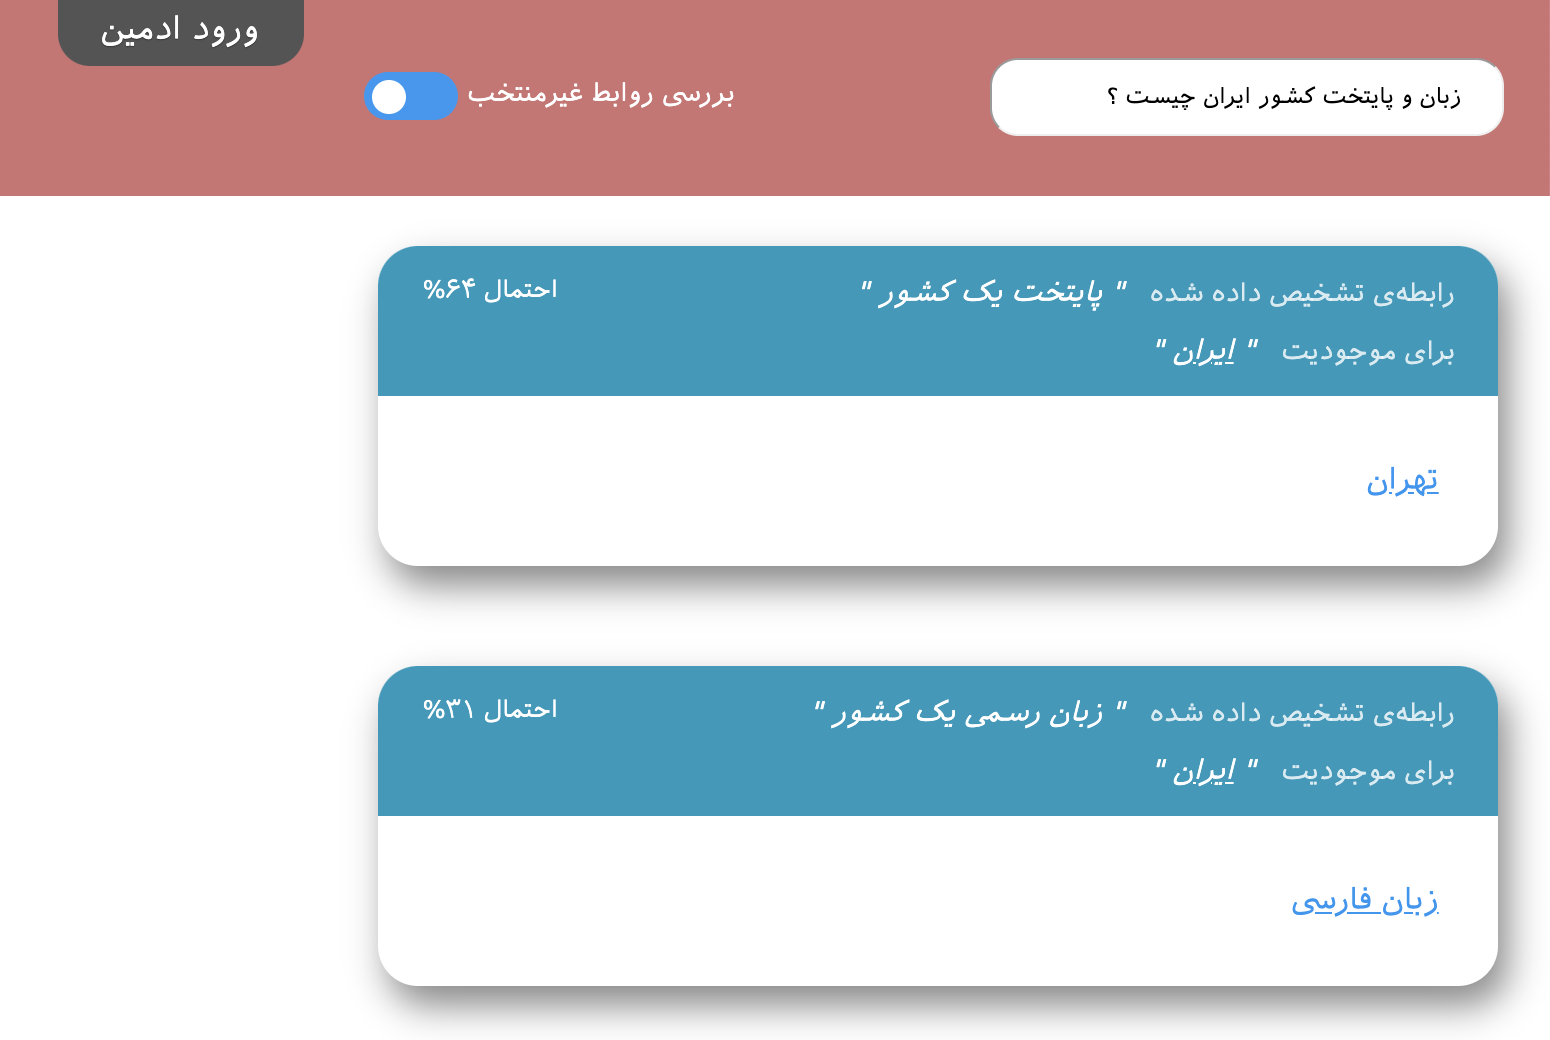
\includegraphics[width=15cm]{figures/interface/user-multiple-rel.png}
	\caption{صفحه کاربر عادی همراه روابط غیرمنتخب}
\end{figure}

\begin{figure}
	\centering
	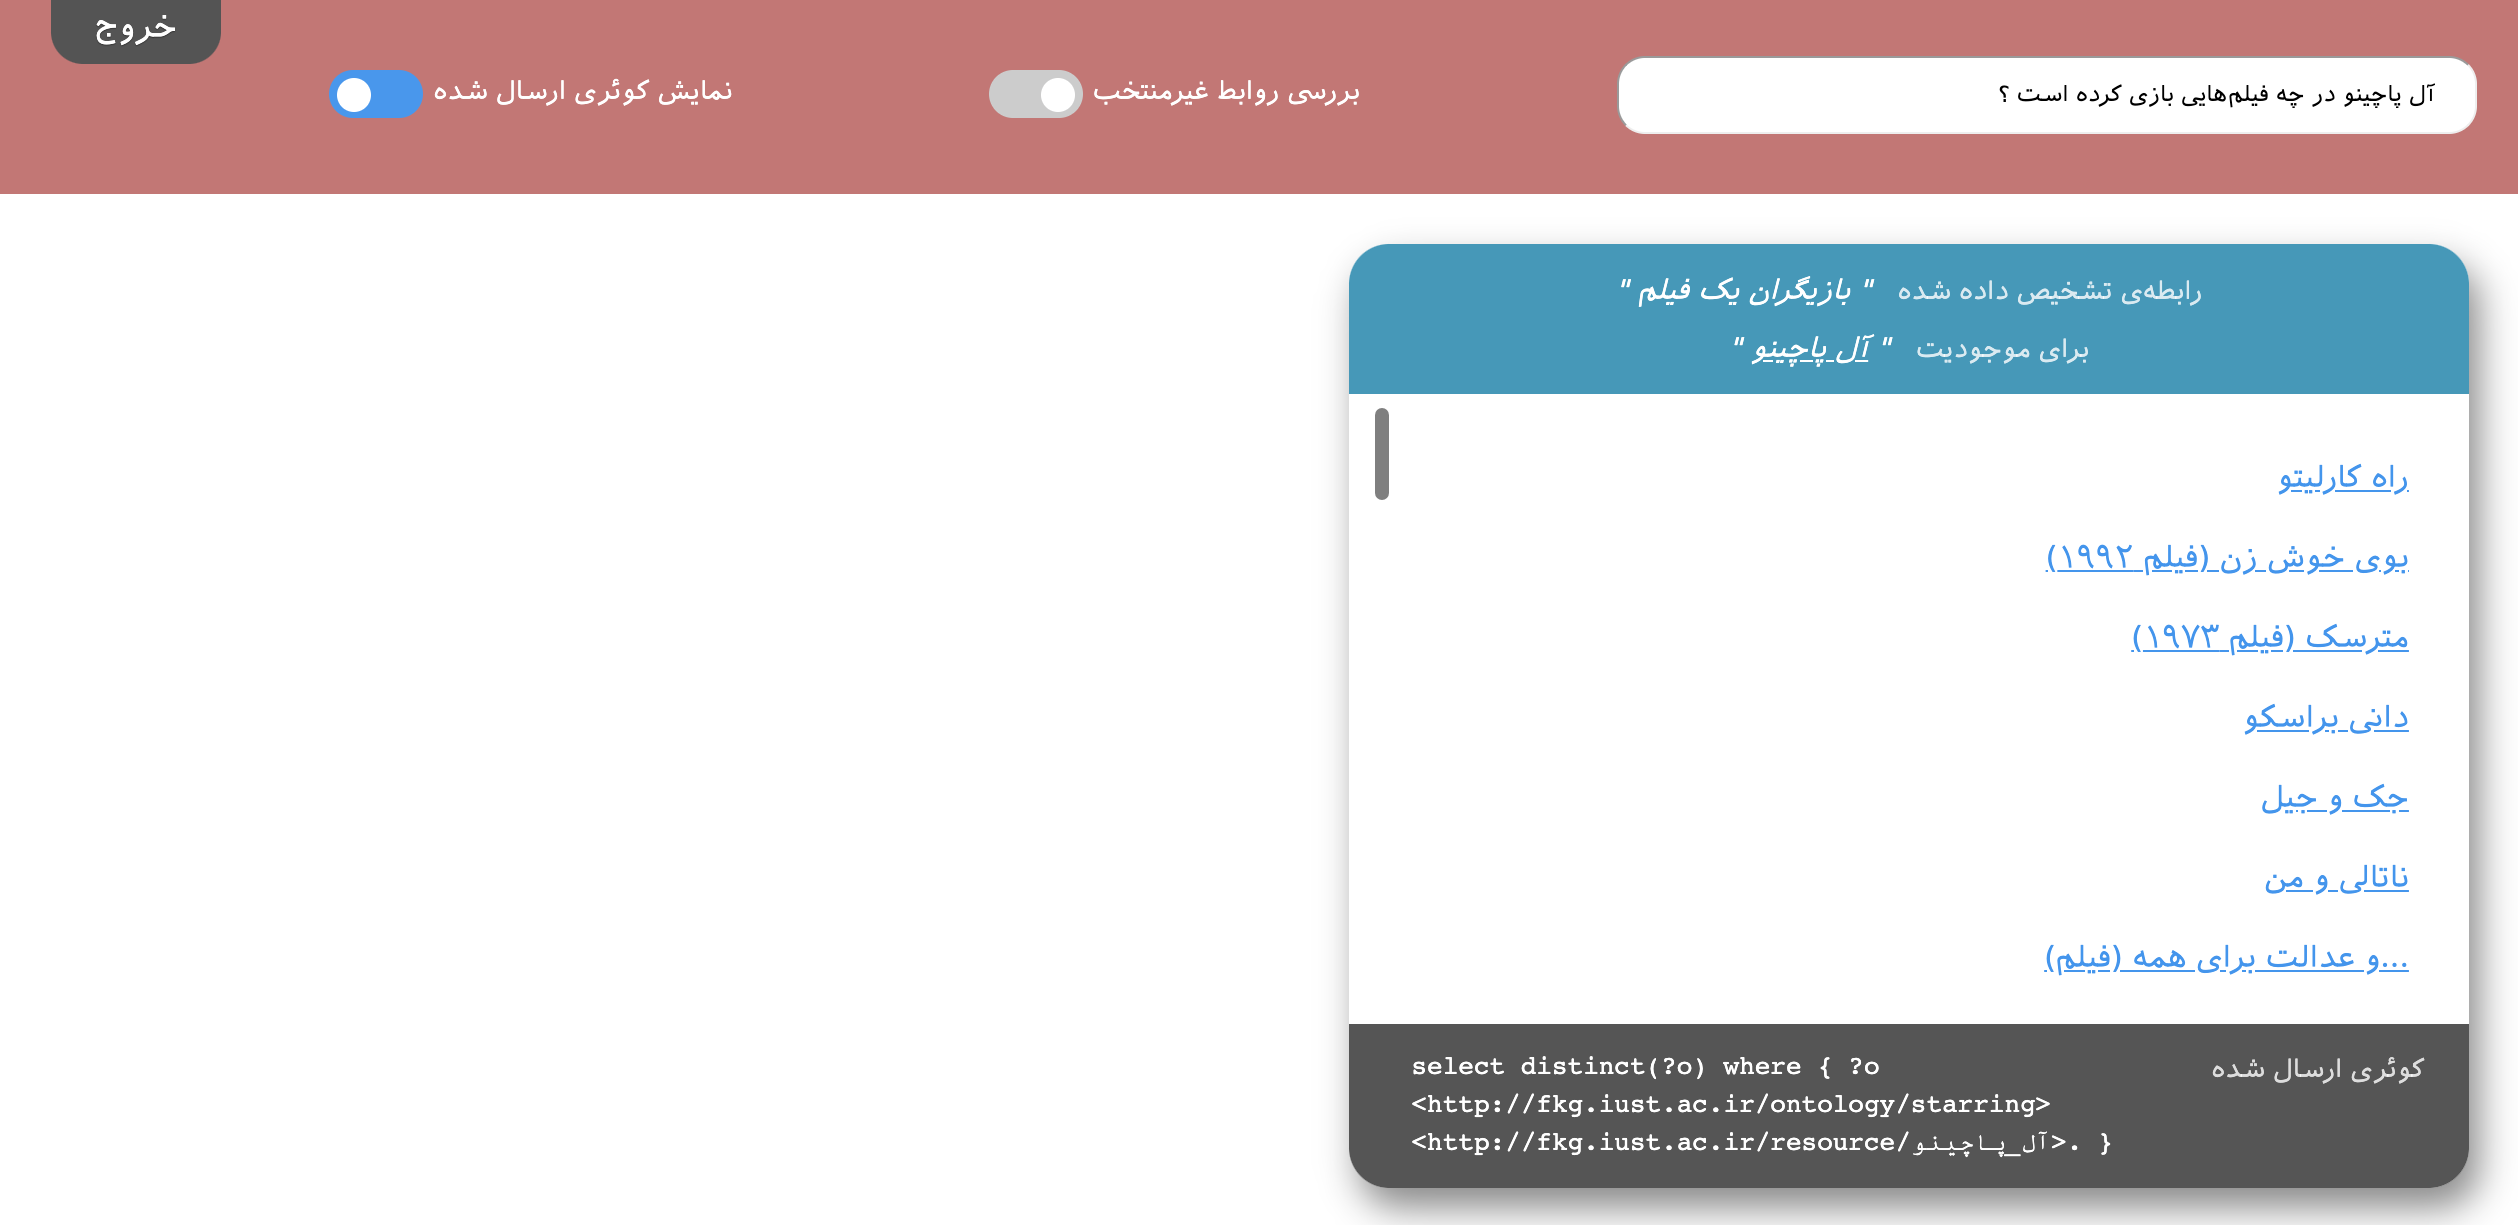
\includegraphics[width=15cm]{figures/interface/admin.png}
	\caption{صفحه کاربر تحلیل‌گر}
\end{figure}

\begin{figure}
	\centering
	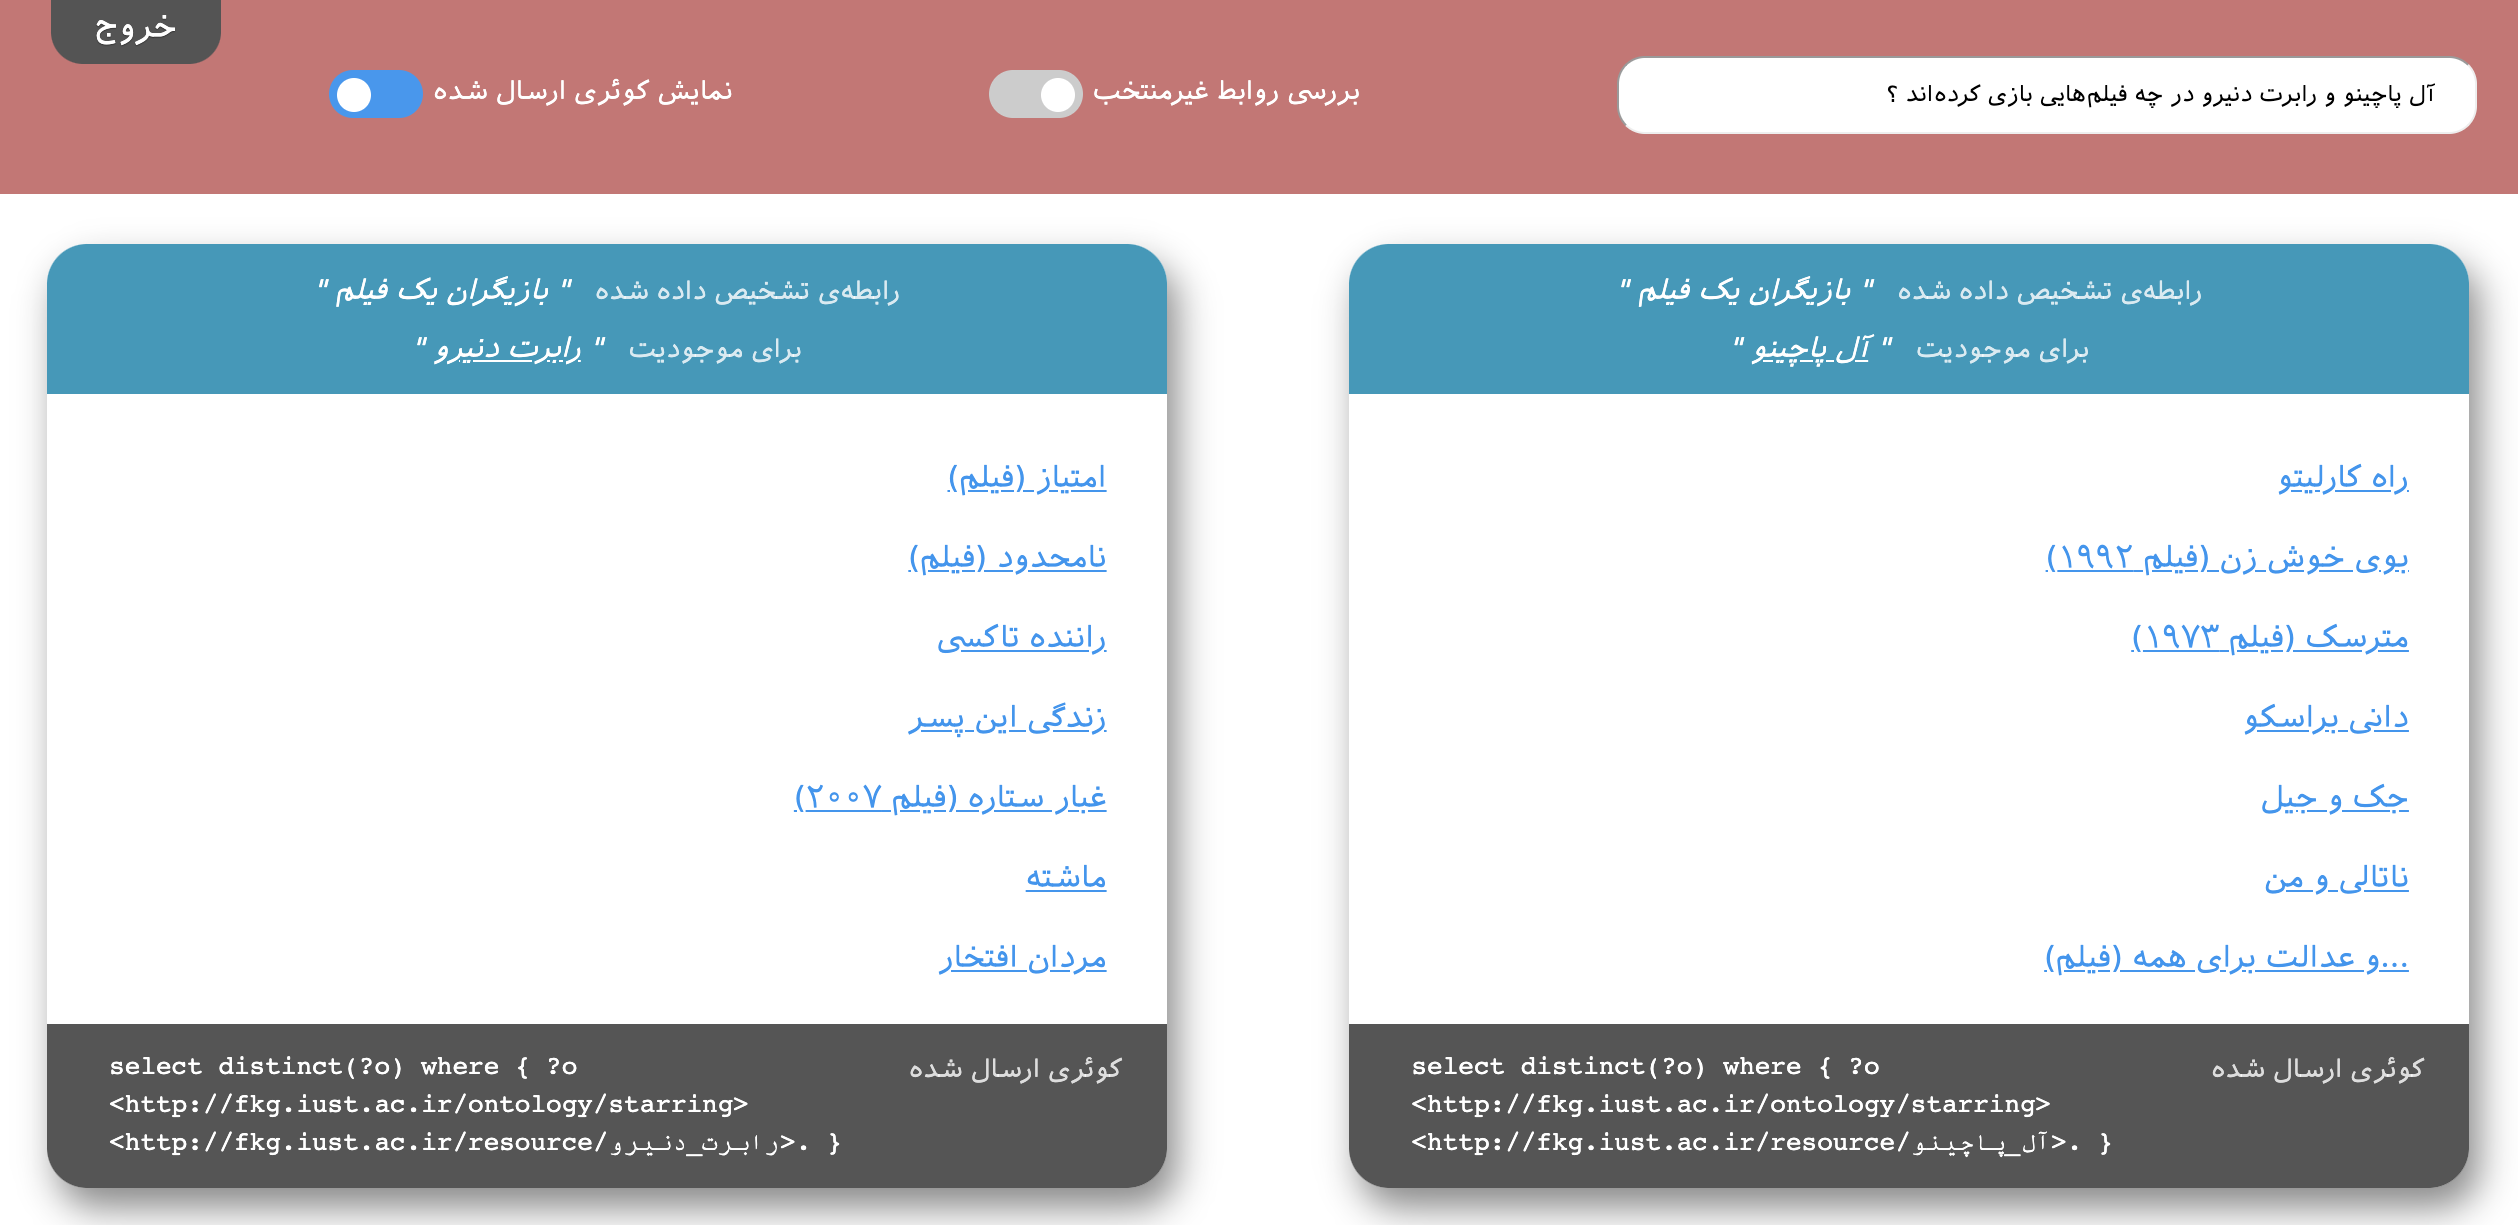
\includegraphics[width=15cm]{figures/interface/admin-multiple-ent.png}
	\caption{صفحه کاربر تحلیل‌گر همراه چند موجودیت}
\end{figure}

\begin{figure}
	\centering
	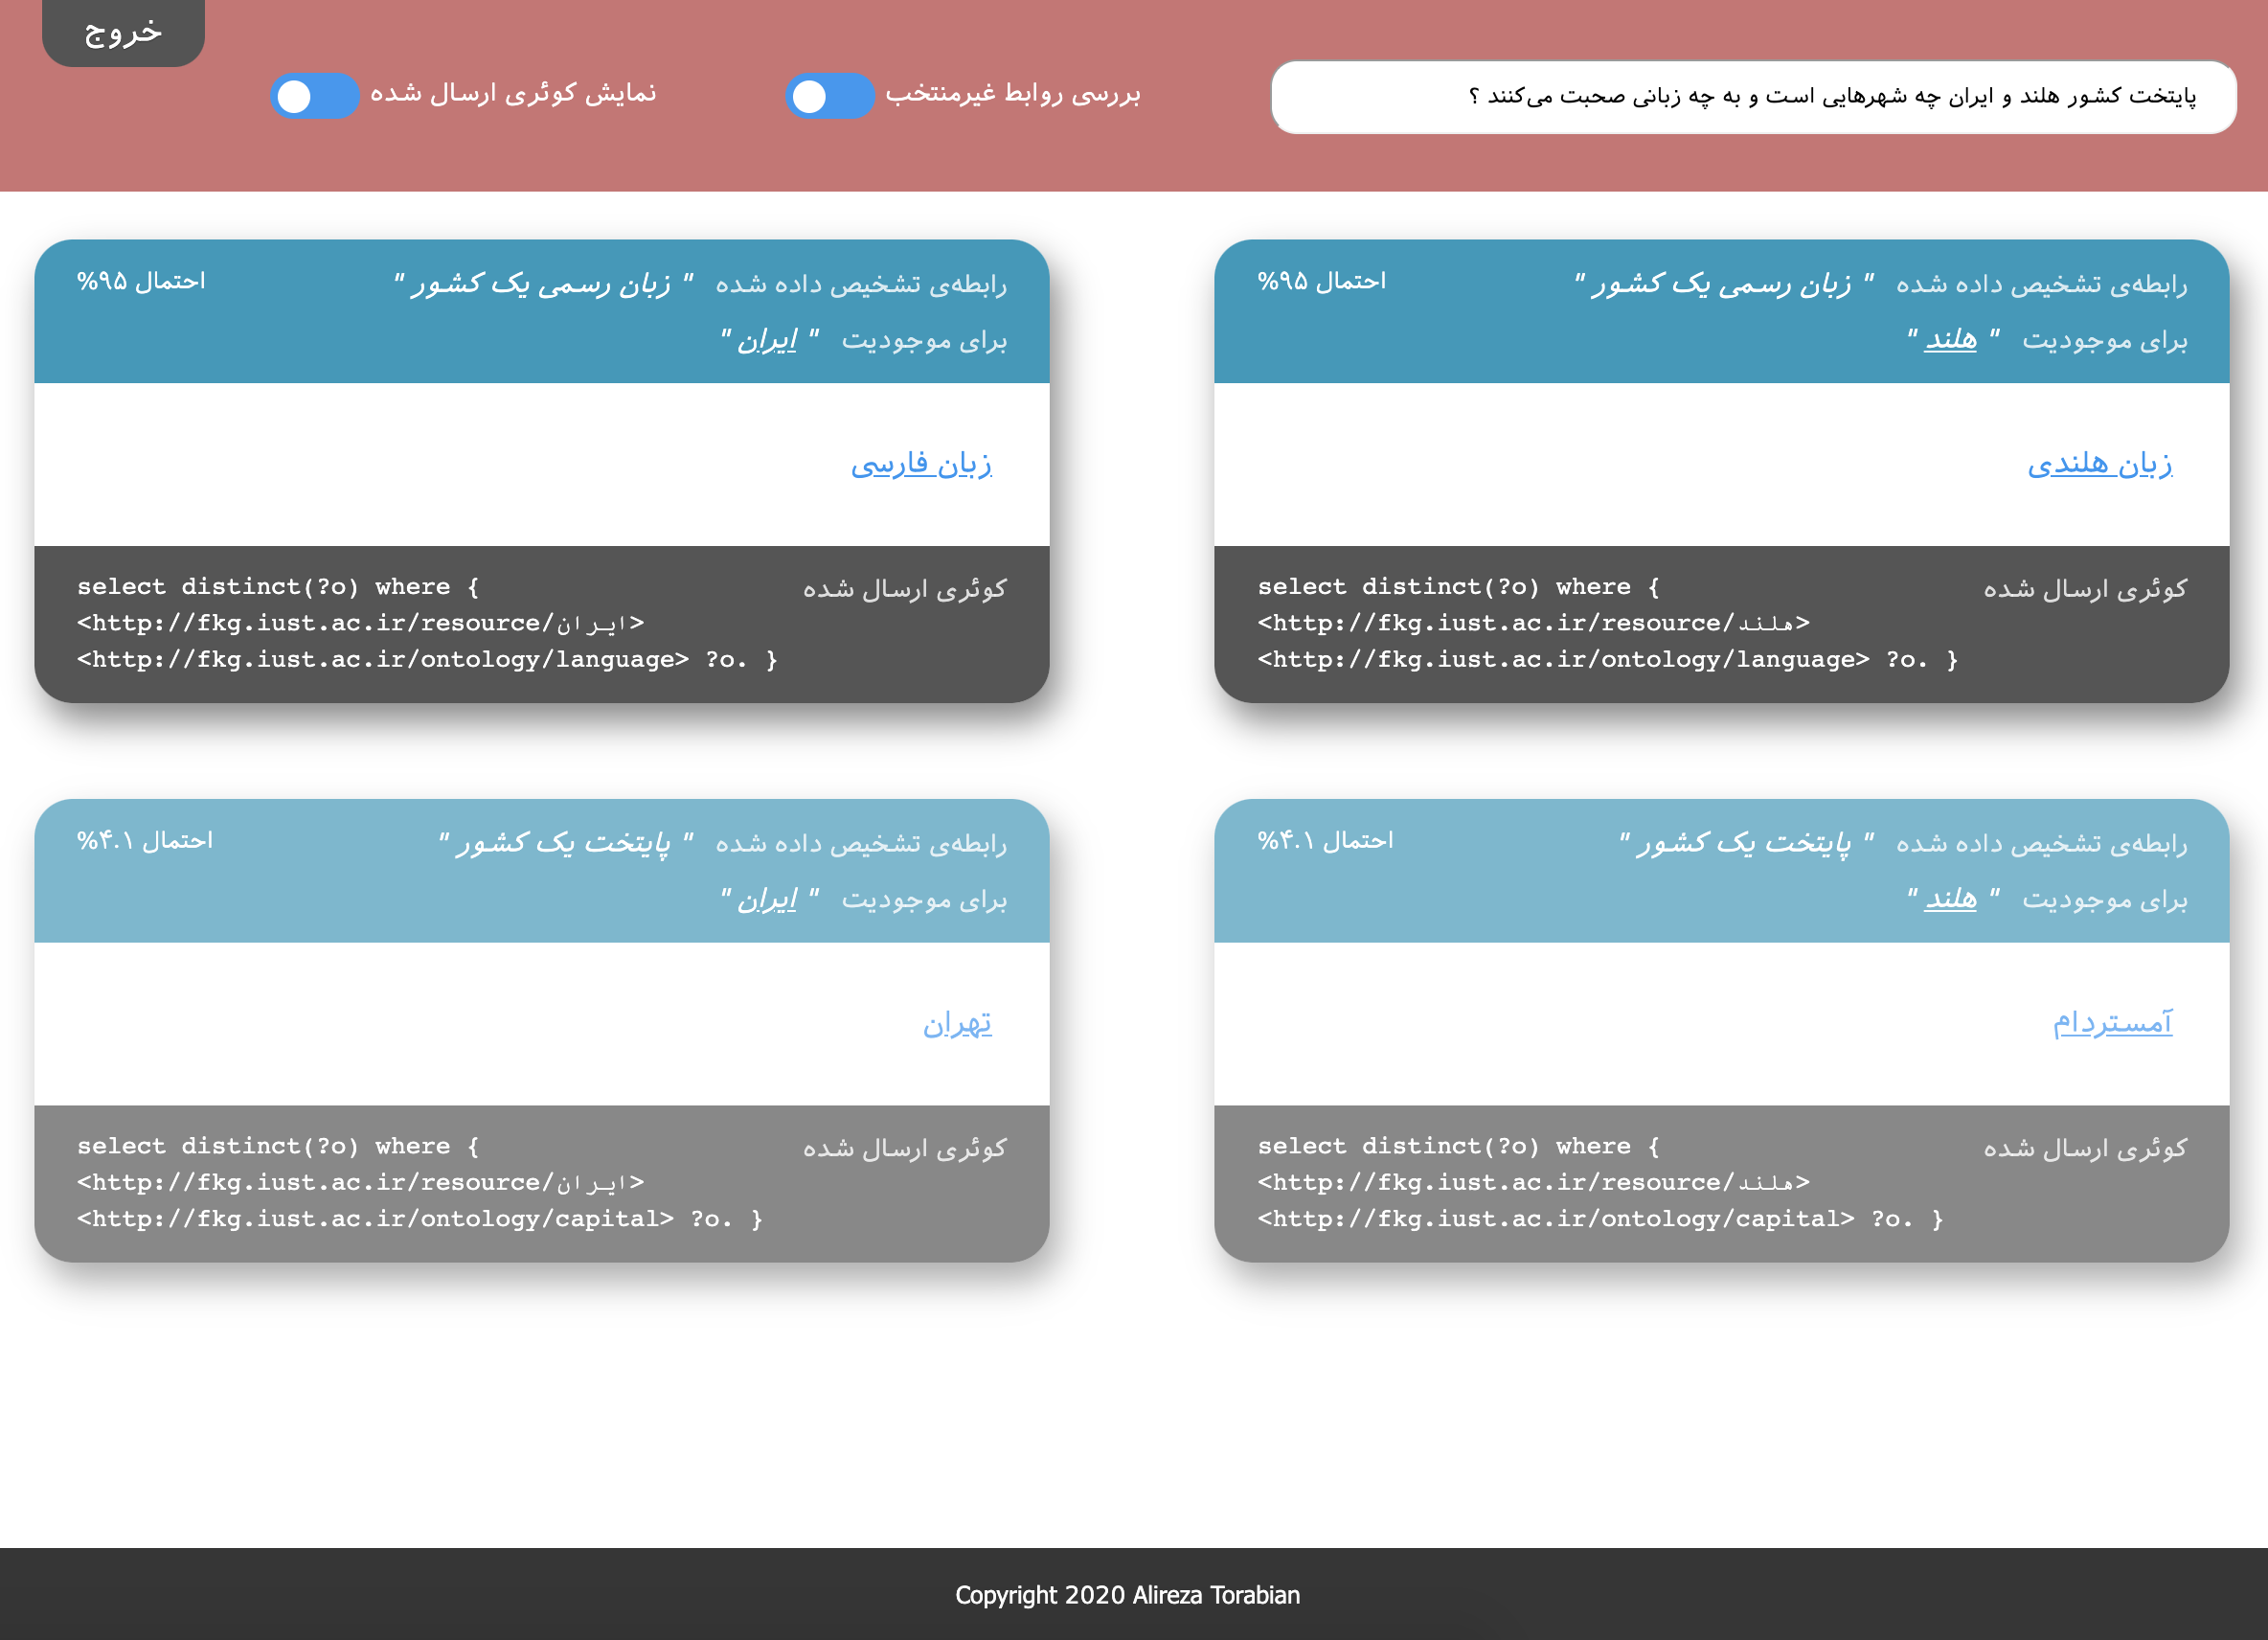
\includegraphics[width=15cm]{figures/interface/admin-double-multiple.png}
	\caption{صفحه کاربر تحلیل‌گر همراه چند موجودیت و روابط غیرمنتخب}
\end{figure}
\chapter{آزمایش و ارزیابی سیستم}
در فصل قبل قسمت‌های مختلف سیستم همراه با مدل‌های مورد استفاده بررسی شدند. در این فصل ابتدا با معیارهای معمول ارزیابی آشنا شده، سپس بخش‌های مختلف موجود در سیستم مورد آزماش قرار گرفته و ارزیابی می‌شوند.
\section{معیارهای ارزیابی}
برای ارزیابی یک دسته‌بند دودویی امکان رخداد چهار حالت شامل منفی درست\footnote{\lr{True Negative (TN)}}، منفی نادرست\footnote{\lr{False Negative (FN)}}، مثبت درست\footnote{\lr{True Positive (TP)}} و مثبت نادرست\footnote{\lr{False Positive (FP)}} وجود دارد که دو حالت از آنها خطا محسوب می‌شوند. این دو حالت حالاتی هستند که خروجی تشخیص داده شده با خروجی واقعی در تضاد باشد و در علم آمار به خطای نوع اول و دوم مشهور می‌باشند. این حالات را در جدول \ref{tab:hypo_test} با نام ماتریس درهم‌ریختگی\footnote{\lr{Confusion Matrix}} مشاهده می‌کنید. در ادامه برای اختصار از نمادهای $TP$، $FP$، $TN$ و $FN$ به ترتیب به نمایندگی از تعداد موارد مثبت درست، مثبت نادرست (خطای نوع اول)، منفی درست و منفی نادرست (خطای نوع دوم) استفاده می‌کنیم.
\\

\begin{table}[h]
	\centering
	\def\arraystretch{1.6}
	\setlength{\tabcolsep}{20pt}
	\begin{tabular}{|c|c|c|}
		\cline{2-3}
		\multicolumn{1}{c|}{} & \cellcolor{headerColor}واقعاً منفی & \cellcolor{headerColor}واقعاً مثبت \\
		\hline
		\cellcolor{headerColor} & منفی درست & منفی نادرست \\
		\multirow{-2}{*}{\cellcolor{headerColor}پیش‌بینی منفی}& & (خطای نوع دوم) \\
		\hline
		\cellcolor{headerColor} & مثبت نادرست & مثبت درست \\
		\multirow{-2}{*}{\cellcolor{headerColor}پیش‌بینی مثبت} & (خطای نوع اول) & \\
		\hline
	\end{tabular}	
	\caption{ماتریس درهم‌ریختگی}
	\label{tab:hypo_test}
\end{table}	

\subsection{صحت}
یکی از ساده‌ترین معیارها برای ارزیابی درستی یک سیستم استفاده از معیار صحت\footnote{\lr{Accuracy}} می‌باشد. درصد صحت سیستم با نسبت گرفتن تعداد پاسخ‌های درست بر تعداد کل پاسخ‌ها بدست می‌آید که رابطه‌ی آنرا در \ref{eqn:accuracy} مشاهده می‌کنید.
\begin{equation}
\label{eqn:accuracy}
Accuracy = \frac{TP + TN}{TP + FP + TN + FN}
\end{equation}
\subsection{دقت و فراخوانی و امتیاز $F_{1}$}
دقت\footnote{\lr{Precision}} و فراخوانی\footnote{\lr{Recall}} دو معیار ارزیابی هستند که بر اساس ماتریس درهم‌ریختگی بدست می‌آیند. \\
دقت به این سوال پاسخ می‌دهد که چه نسبتی از موارد انتخابی، مرتبط هستند. مقدار دقت برابر است با نسبت تعداد مواردی که سیستم به درستی تشخیص داده بر تعداد کل مواردی که سیستم تشخیص داده است.\\
فراخوانی به این سوال پاسخ می‌دهد که چه نسبتی از موارد مرتبط، انتخاب شده‌اند. مقدار فراخوانی برابر است با نسبت تعداد مواردی که سیستم به درستی تشخیص داده بر تعداد کل مواردی که سیستم باید تشخیص می‌داده است.\\
روابط دقت و فراخوانی را به ترتیب در \ref{eqn:precision} و \ref{eqn:recall} مشاهده می‌کنید.

\begin{center}
	\begin{minipage}[b]{.45\textwidth}
		\begin{equation}
			\label{eqn:precision}
			Precision = \frac{TP}{TP + FP}
		\end{equation}
	\end{minipage}
	\quad
	\begin{minipage}[b]{.45\textwidth}
		\begin{equation}
			\label{eqn:recall}
			Recall = \frac{TP}{TP + FN}
		\end{equation}
	\end{minipage}
\end{center}
~\\
در بسیاری از موارد نمی‌توان با استناد به معیار صحت درستی یک سیستم را بررسی کرد. به عنوان مثال سیستمی را در نظر بگیرید که هدف آن تشخیص یک بیماری خاص می‌باشد. از آنجا که درصد بسیار کمی از افراد دارای این بیماری هستند اگر سیستم به ازای همه‌ی ورودی‌ها عدم بیماری را تشخیص دهد، درصد صحت بسیار بالایی خواهد داشت در صورتی که چنین سیستمی اصلا کارایی ندارد. در چنین سیستم‌هایی معیارهای دقت و فراخوانی کاربردی هستند.\\
معیار $F_{1}$\footnote{\lr{F1-Score}} نوعی میانگین بین معیارهای دقت و فراخوانی است. برای مقایسه‌ی دو سیستم با معیار دقت و فراخوانی می‌توان در یک نگاه معیار $F_{1}$ دو سیستم را مقایسه کرد. رابطه‌ی این معیار را در \ref{eqn:f1_score} مشاهده می‌نمایید.
\begin{equation}
\label{eqn:f1_score}
F_{1} = \frac{2 * Precision * Recall}{Precision + Recall}
\end{equation}

\subsubsection{دقت و فراخوانی و امتیاز $F_{1}$ برای دسته‌بندهایی با چند کلاس}
برای مسائلی با چند کلاس می‌توان معیارهای دقت و فراخوانی را برای هر کلاس به صورت جداگانه محاسبه نمود. در این مسائل مقدار دقت یک کلاس برابر است با نسبت تعداد مواردی که سیستم به درستی آن کلاس را تشخیص داده بر تعداد کل مواردی که سیستم برای آن کلاس تشخیص داده است. مقدار فراخوانی برابر است با نسبت تعداد مواردی که سیستم به درستی برای آن کلاس تشخیص داده بر تعداد کل مواردی که عضو در این کلاس می‌باشد.\\
برای بدست آورد یک مقدار واحد برای دقت یا فراخوانی می‌توان میانگین میکرو\footnote{\lr{Micro Average}} یا میانگین ماکروی\footnote{\lr{Macro Average}} این معیارها را محاسبه نمود.
برای بدست آوردن میانگین ماکرو ابتدا مقدار دقت و یا فراخوانی هر کلاس جداگانه حساب شده و میانگین آنها محاسبه می‌شود.
اما برای محاسبه‌ی میانگین میکرو تعداد موارد مثبت یا منفی درست یا نادرست برای هر کلاس محاسبه شده و از مجموع همگی آنها طبق فرمول دقت و فراخوانی استفاده می‌شود. در ادامه روابط این دو میانگین برای معیار‌های دقت و فراخوانی را برای یک دسته‌بند با $n$ کلاس مشاهده می‌کنید. در این روابط برای تفکیک تعداد موارد هر حالت از پاسخ‌های هر کلاس از اندیس استفاده شده است. به عنوان مثال منظور از $TP_i$ تعداد موارد مثبت درست برای کلاس $i$ام می‌باشد.
\begin{center}
	\begin{minipage}[b]{.45\textwidth}
		\begin{equation}
		\label{eqn:precision_macro}
		(\sum_{i = 1}^{n} \frac{TP_i}{TP_i + FP_i}) / n
		\end{equation}
		\centerline{\small{میانگین ماکرو معیار دقت}}
	\end{minipage}
	\quad
	\begin{minipage}[b]{.45\textwidth}
		\begin{equation}
		\label{eqn:recall_macro}
		(\sum_{i = 1}^{n} \frac{TP_i}{TP_i + FN_i}) / n
		\end{equation}
		\centerline{\small{میانگین ماکرو معیار فراخوانی}}
	\end{minipage}
\end{center}

\begin{center}
	\begin{minipage}[b]{.45\textwidth}
		\begin{equation}
		\label{eqn:pp}
		\frac{\sum_{i = 1}^{n} TP_i}{\sum_{i = 1}^{n} (TP_i + FP_i)}
		\end{equation}
		\centerline{\small{میانگین میکرو معیار دقت}}
	\end{minipage}
	\quad
	\begin{minipage}[b]{.45\textwidth}
		\begin{equation}
		\label{eqn:f12_score}
		\frac{\sum_{i = 1}^{n} TP_i}{\sum_{i = 1}^{n} (TP_i + FN_i)}
		\end{equation}
		\centerline{\small{میانگین میکرو معیار فراخوانی}}
	\end{minipage}
\end{center}
در بررسی چنین مسائلی با چند کلاس باز هم می‌توان از مقدار بدست آمده از میانگین دقت و فراخوانی استفاده کرد و طبق فرمول گفته شده امتیاز $F_1$ را برای آن مسئله محاسبه نمود. در ارزیابی دسته‌بندهای این پروژه از میانگین ماکرو استفاده می‌شود.
\section{روش اعتبارسنجی متقابل}
اعتبارسنجی متقابل\footnote{\lr{Cross Validation}} یک روش ارزیابی مدل است که تعیین می‌نماید نتایج یک تحلیل آماری بر روی یک مجموعه ‌داده تا چه اندازه قابل تعمیم و مستقل از داده‌های آموزشی است و چه مقدار می‌تواند در مقابل داده‌های جدید به درستی عمل کند. این روش به ‌طور ویژه در کاربردهای پیش‌بینی مورد استفاده قرار می‌گیرد تا مشخص شود مدل مورد نظر تا چه اندازه در عمل مفید خواهد بود. به ‌طور کلی یک دور از اعتبارسنجی متقابل شامل افراز داده‌ها به دو زیرمجموعه مکمل تحت عنوان مجموعه‌ی آموزش و مجموعه‌ی اعتبارسنجی یا آزمایش، انجام آموزش روی زیرمجموعه‌ی آموزش و سپس ارزیابی توسط مجموعه‌ی دیگر است. برای کاهش پراکندگی\footnote{\lr{Variability}} در نتایج، عمل اعتبارسنجی چندین بار با افرازهای مختلف انجام شده و از نتایج اعتبارسنجی‌ها میانگین گرفته می‌شود. با افزایش تعداد افرازها پراکندگی نتایج کاهش میابد \cite{seni2010ensemble}.

\subsection{اعتبارسنجی متقابل چندتایی}
در روش اعتبارسنجی متقابل چندتایی یا $k$تایی\footnote{\lr{K-Fold}} داده‌های اصلی به صورت رندم به $k$ زیرمجموعه با اندازه‌ی مساوی تقسیم می‌شود. فرایند آزمایش در $k$ مرحله انجام می‌شود. در مرحله‌ی $i$ام زیرمجموعه‌ی $i$ام به عنوان مجموعه‌ی آزمایش و سایر داده‌ها به عنوان مجموعه‌ی آموزش در نظر گرفته شده و آموزش مدل و سپس ارزیابی آن انجام می‌شود. در نهایت میانگین نتایج این آزمایش‌ها محاسبه شده و به عنوان معیار ارزیابی مدل استفاده می‌شود.
مزیت این روش در این است که هر یک از داده‌ها به طور برابر برای آموزش و آزمایش استفاده می‌شوند.
\section{نتایج ارزیابی سیستم}
سیستم پیاده‌سازی شده در این پروژه دارای دو قسمت اصلی دسته‌بند رابطه و تشخیص‌دهنده‌ی موجودیت می‌باشد. در این بخش هر کدام از این بخش‌ها و همچنین کل سیستم به صورت یکپارچه مورد آزمایش قرار گرفته شده و داده‌هایی که منجر به نتیجه‌ی غلط می‌شدند، استخراج شده و مورد تحلیل قرار گرفته‌اند. برنامه‌های مربوط به ارزیابی بخش‌های مختلف سیستم در پکیج \lr{evaluation} پیاده‌سازی شده‌اند.
\subsection{ارزیابی دسته‌بندهای رابطه}
همانطور که در فصل‌های قبل توضیح داده شد در این سیستم از دو دسته‌بند ماشین بردار پشتیبان و شبکه عصبی پیچشی استفاده می‌شود. نتایج آزمایش هر دو دسته‌بند را در ادامه مشاهده می‌کنید.\\
هر کدام از دسته‌بندها همراه روش تعبیه‌سازی خود در پنج روش مورد آزمایش قرار گرفته‌اند. روش اول روش اعتبارسنجی متقابل چندتایی با تعداد ۵ زیرمجموعه است. برای چهار روش بعدی مجموعه داده‌های اصلی با نسبت ۴، ۱، ۱ به سه قسمت آموزش، اعتبارسنجی و آزمایش تقسیم شده‌اند. در اولین این روش‌ها مجموعه داده‌ها به صورت کاملا رندم تقسیم می‌شوند. در روش بعدی مجموعه داده‌ها طوری تقسیم می‌شوند که الگوی داده‌های مجموعه‌ی آموزش در دو مجموعه‌ی دیگر تکرار نشود. دو روش بعدی به ترتیب همانند روش‌های ذکر شده هستند اما با این تفاوت که روابط یک جهته شده‌اند. به عنوان مثل در مجموعه‌ی عادی رابطه‌ی "پایتخت یک کشور" وجود دارد اما در روابط یک‌جهته به ازای آن، دو رابطه‌ی "پایتخت یک کشور۱" و "پایتخت یک کشور۲" وجود دارد که تفاوت آنها در این است که یکی از آنها رابطه از موجودیت کشور به شهر است و دیگری برعکس. در چنین حالتی تشخیص برای دسته‌بند سخت‌تر می‌شود. این پنج روش را به طور خلاصه در ادامه مشاهده می‌نمایید:
\begin{itemize}
	\item ۵تایی\footnote{\lr{$5$-Fold}}
	\item مجموعه داده
	\item مجموعه داده - الگو متمایز
	\item مجموعه داده - یک‌جهته
	\item مجموعه داده - یک‌جهته - الگو متمایز
\end{itemize}
\subsubsection{ماشین بردار پشتیبان}
در جدول \ref{tab:svm_evaluation} نتایج ارزیابی دسته‌بند ماشین بردار پشتیبان را مشاهده می‌کنید.
\begin{table}[h]
	\centering
	\def\arraystretch{1.3}
	\setlength{\tabcolsep}{7pt}
	\begin{tabular}{|c|c|>{\setlatin}c|>{\setlatin}c|>{\setlatin}c|>{\setlatin}c|}
		\hline
		\rowcolor{headerColor}
		 & && دقت & فراخوانی &
		\\
		\rowcolor{headerColor}
		\multirow{-2}{*}{روش آزمایش}&\multirow{-2}{*}{روش تعبیه‌سازی}&\multirow{-2}{*}{~صحت~} &(میانگین ماکرو)&(میانگین ماکرو)&\multirow{-2}{*}{امتیاز$F_{1}$}
		\\ \hline
		\multirow{4}{*}{۵تایی} &\lr{BOW}&99.49&99.35&98.88&99.12
	\\
	&\lr{TF-IDF}&99.62&99.47&99.15&99.31
	\\
	&\lr{word2vec}&99.63&99.35&99.31&99.33
	\\
	&\lr{word2vec} وزن‌دار&99.57&99.34&99.10&99.22
	\\ \hline
	
	\multirow{4}{*}{مجموعه داده} &\lr{BOW}&99.36&99.32&98.58&98.95
	\\
	&\lr{TF-IDF}&99.48&99.34&98.87&99.10
	\\
	&\lr{word2vec}&99.46&99.16&98.89&99.02
	\\
	&\lr{word2vec} وزن‌دار&99.49&99.36&98.89&99.12
	\\ \hline
	
	&\lr{BOW}&98.76&98.33&97.58&97.96
	\\
	مجموعه داده&\lr{TF-IDF}&98.63&97.38&97.00&97.19
	\\
	الگو متمایز&\lr{word2vec}&98.57&97.54&97.19&97.36
	\\
	&\lr{word2vec} وزن‌دار&98.10&96.52&95.88&96.20
	\\ \hline
	
	&\lr{BOW}&98.27&97.93&96.17&97.04
	\\
	مجموعه داده&\lr{TF-IDF}&99.08&98.52&98.05&98.29
	\\
	یک‌جهته&\lr{word2vec}&98.95&98.37&98.10&98.23
	\\
	&\lr{word2vec} وزن‌دار&98.66&98.07&97.49&97.78
	\\ \hline
	
	\multirow{4}{*}{\begin{tabular}{@{}c@{}c@{}}مجموعه داده\\یک‌جهته\\الگو متمایز\end{tabular}}
	&\lr{BOW}&96.67&95.17&93.47&94.31
	\\
	&\lr{TF-IDF}&97.06&94.55&94.01&94.28
	\\
	&\lr{word2vec}&95.96&92.67&92.86&92.76
	\\
	&\lr{word2vec} وزن‌دار&95.38&91.19&90.65&90.92
	\\ \hline
	
	\end{tabular}	
	\caption{ارزیابی دسته‌بند ماشین بردار پشتیبان}
	\label{tab:svm_evaluation}
\end{table}
\\
در جدول \ref{tab:svm_troubled_samples} نمونه‌هایی از داده‌های مشکل‌دار مربوط به این دسته‌بند را مشاهده می‌کنید. عمده مشکل این دسته‌بند در تشخیص داده‌های کلاس‌هایی بوده که حاوی کلمات مشترک زیادی در جملات آموزششان بوده‌اند.
\begin{table}[H]
	\centering
	\def\arraystretch{1.3}
	\begin{tabularx}{\linewidth}{|L|c|c|}
		\hline
		\rowcolor{headerColor}
		\multicolumn{1}{|c|}{پرسش}&رابطه‌ی هدف&رابطه‌ی تشخیص داده شده
		\\ \hline
		\small{سوتن کورو نویسنده اش چه نام دارد}&نویسنده یک فیلم&نویسنده کتاب
		\\ \hline
		\small{چه کسی فیلم جزیره مرده ۲ را کارگردانی می کند}&کارگردان یک سریال تلویزیونی&کارگردان یک فیلم
		\\ \hline
	\end{tabularx}	
	\caption{نمونه‌های مشکل‌دار دسته‌بند ماشین بردار پشتیبان}
	\label{tab:svm_troubled_samples}
\end{table}

\subsubsection{شبکه عصبی پیچشی}
برای آموزش نهایی این شبکه فرایند آموزش روی داده‌ها در ۱۰ دوره\footnote{\lr{Epoch}} انجام شده است. برای تحلیل عملکرد این شبکه مقدار صحت و تابع هزینه‌ی این شبکه طی دوره‌های ۱ تا ۱۵ استخراج شده‌اند که در جدول \ref{tab:cnn_training} قرار گرفته‌اند. همانطور که در فصل گذشته گفته شده بود از تابع هزینه‌ی \lr{Categorical Cross-Entropy} برای آموزش این شبکه می‌شود. نمودار صحت و هزینه‌ را در شکل‌های \ref{fig:cnn_training_acc} و \ref{fig:cnn_training_loss} مشاهده می‌کنید.
\begin{table}[H]
	\centering
	%\def\arraystretch{1.3} 
	\begin{tabular}{|C{.6cm}|>{\setlatin}C{1.3cm}|>{\setlatin}C{1.3cm}|}
		\hline
		\rowcolor{headerColor}
		دوره&صحت&هزینه
		\\ \hline
		1&94.45&0.2224
		\\ \hline
		2&98.71&0.0734
		\\ \hline
		3&99.05&0.0607
		\\ \hline
		4&99.22&0.0553
		\\ \hline
		5&99.31&0.0525
		\\ \hline
		6&99.35&0.0501
		\\ \hline
		7&99.38&0.0477
		\\ \hline
	\end{tabular}
	\begin{tabular}{|C{.6cm}|>{\setlatin}C{1.3cm}|>{\setlatin}C{1.3cm}|}
		 \hline
		8&99.46&0.0485
		\\ \hline
		9&99.48&0.0442
		\\ \hline
		10&99.52&0.0405
		\\ \hline
		11&99.52&0.0455
		\\ \hline
		12&99.55&0.0394
		\\ \hline
		13&99.53&0.0470
		\\ \hline
		14&99.57&0.0424
		\\ \hline
		15&99.61&0.0401
		\\ \hline
		
	\end{tabular}	
	\caption{صحت و هزینه‌ی شبکه عصبی پیچشی}
	\label{tab:cnn_training}
\end{table}

\begin{multicols}{2}
	\begin{figure}[H]
		\centering
		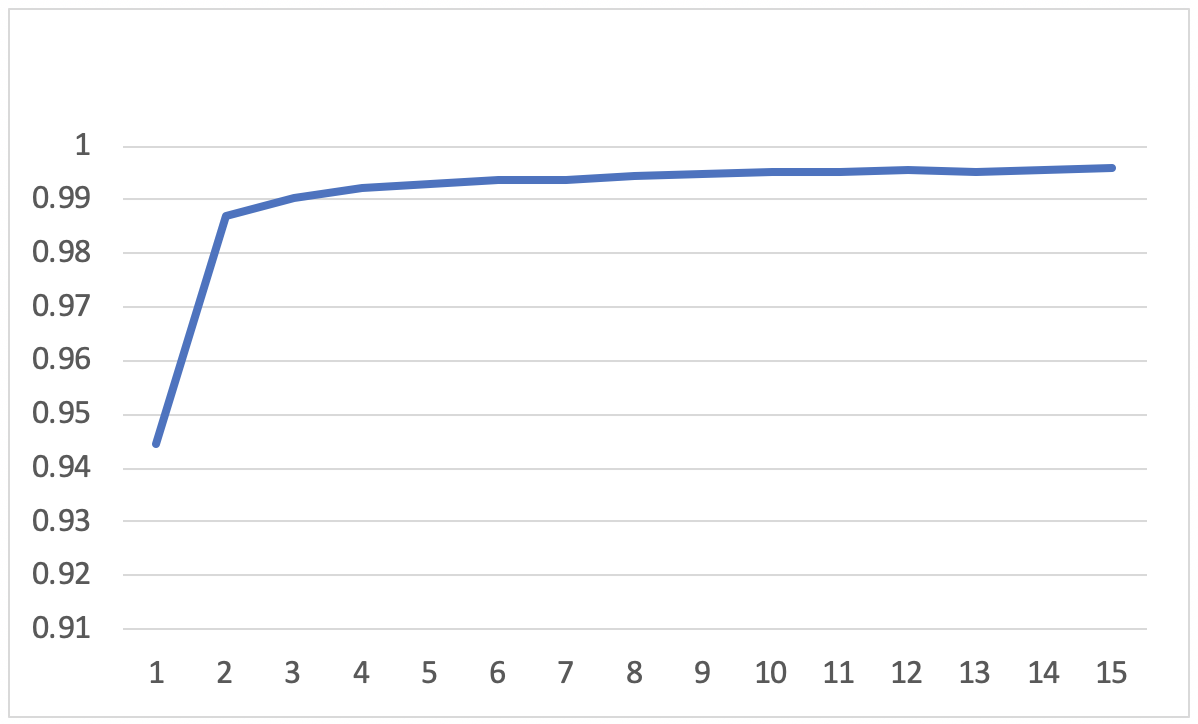
\includegraphics[width=7cm]{figures/cnn/training/accuracy.png}
		\caption{صحت شبکه دسته‌بند}
		\label{fig:cnn_training_acc}
	\end{figure}
	\columnbreak
	\begin{figure}[H]
		\centering
		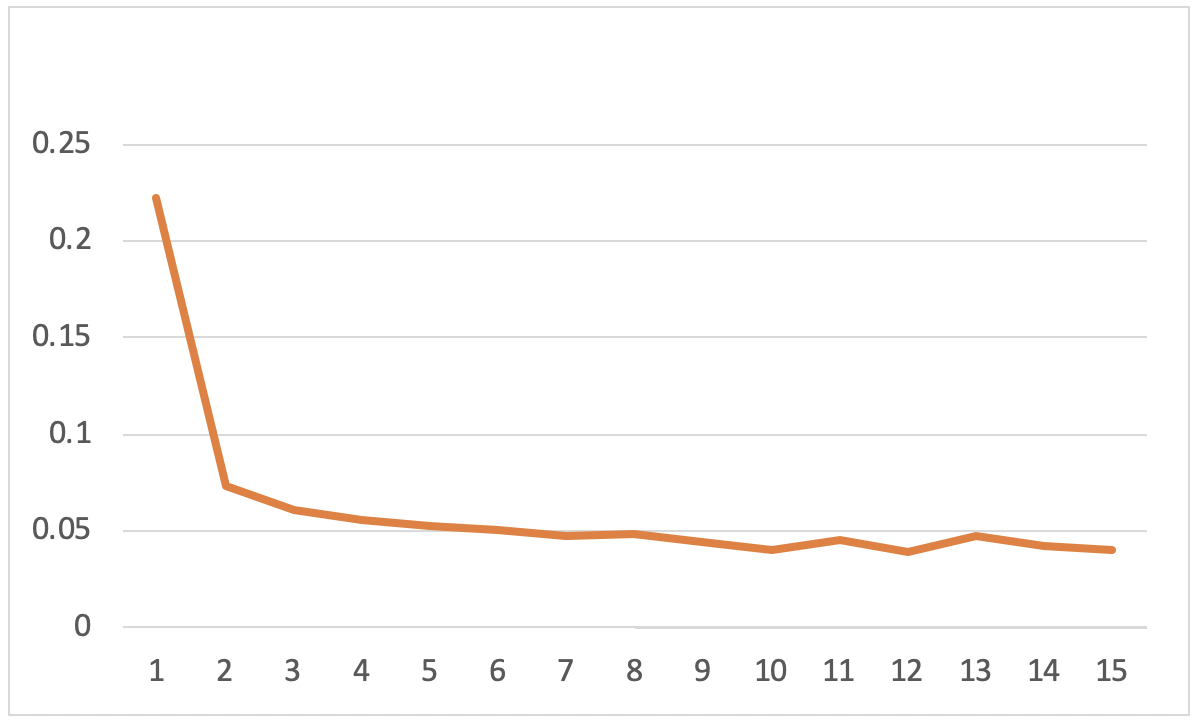
\includegraphics[width=7cm]{figures/cnn/training/loss.png}
		\caption {هزینه‌ی شبکه دسته‌بند}
		\label{fig:cnn_training_loss}
	\end{figure}
\end{multicols}

\noindent در جدول \ref{tab:cnn_evaluation} نتایج ارزیابی دسته‌بند شبکه عصبی پیچشی را مشاهده می‌کنید. از آنجا که روش تعبیه‌سازی استفاده شده در این دسته‌بند یعنی روش \lr{word2vec}، یکی از روش‌های تعبیه‌سازی مورد استفاده در دسته‌بند ماشین بردار پشتبیان نیز می‌باشد، برای مقایسه، نتایج آزمایش مربوط به این روش تعبیه‌سازی در دسته‌بند ماشین بردار پشتبیان که در جدول \ref{tab:svm_evaluation} بیان شدند در جدول \ref{tab:cnn_evaluation} نیز آورده شده‌اند.
با مقایسه‌ی نتایج این دو دسته‌بند مشخص می‌شود که در اکثر آزمایش‌ها و روش‌ها شبکه عصبی پیچشی عملکرد نسبتاً بهتری را داشته است.
\begin{table}[h]
	\centering
	\def\arraystretch{0.85}
	\setlength{\tabcolsep}{9pt}
	\begin{tabular}{|c|c|>{\setlatin}c|>{\setlatin}c|>{\setlatin}c|>{\setlatin}c|}
		\hline
		\rowcolor{headerColor}
		& & & دقت & فراخوانی & 
		\\
		\rowcolor{headerColor}
		\multirow{-2}{*}{روش آزمایش}&\multirow{-2}{*}{نوع دسته‌بند}&\multirow{-2}{*}{~صحت~}&(میانگین ماکرو)&(میانگین ماکرو)&\multirow{-2}{*}{امتیاز $F_{1}$}
		\\ \hline
	
		&\lr{CNN}&\begin{tabular}{@{}c@{}c@{}}‌~\\99.72\\~\end{tabular}&99.55&99.49&99.52
		\\
		\multirow{-4}{*}{۵تایی}
		&\lr{SVM}&\begin{tabular}{@{}c@{}c@{}}‌~\\99.63\\~\end{tabular}&99.35&99.31&99.33
		\\ \hline
		
		&\lr{CNN}&\begin{tabular}{@{}c@{}c@{}}‌~\\99.66\\~\end{tabular}&99.44&99.37&99.40
		\\
		\multirow{-4}{*}{مجموعه داده}
		&\lr{SVM}&\begin{tabular}{@{}c@{}c@{}}‌~\\99.46\\~\end{tabular}&99.16&98.89&99.02
		\\ \hline
		
		&\lr{CNN}&\begin{tabular}{@{}c@{}c@{}}‌~\\98.24\\~\end{tabular}&96.49&96.63&96.56
		\\
		\multirow{-4}{*}{\begin{tabular}{@{}c@{}}مجموعه داده\\الگو متمایز\end{tabular}}
		&\lr{SVM}&\begin{tabular}{@{}c@{}c@{}}‌~\\98.57\\~\end{tabular}&97.54&97.19&97.36
		\\ \hline
		
		&\lr{CNN}&\begin{tabular}{@{}c@{}c@{}}‌~\\99.60\\~\end{tabular}&99.49&99.32&99.40
		\\
		\multirow{-4}{*}{\begin{tabular}{@{}c@{}}مجموعه داده\\یک‌جهته\end{tabular}}
		&\lr{SVM}&\begin{tabular}{@{}c@{}c@{}}‌~\\98.95\\~\end{tabular}&98.37&98.10&98.23
		\\ \hline
		
		&\lr{CNN}&\begin{tabular}{@{}c@{}c@{}}‌~\\96.65\\~\end{tabular}&93.69&93.20&93.45
		\\ 
		\multirow{-4}{*}{\begin{tabular}{@{}c@{}c@{}}مجموعه داده\\یک‌جهته\\الگو متمایز\end{tabular}}
		&\lr{SVM}&\begin{tabular}{@{}c@{}c@{}}‌~\\95.96\\~\end{tabular}&92.67&92.86&92.76
		\\ \hline
	\end{tabular}	
	\caption[ارزیابی دسته‌بندها در روش تعبیه‌سازی \lr{word2vec}]{ارزیابی دسته‌بند شبکه عصبی پیچشی و ماشین بردار پشتیبان که از روش تعبیه‌سازی \lr{word2vec} استفاده کرده‌اند. این دو دسته‌بند به اختصار و به ترتیب با نام‌های \lr{CNN} و \lr{SVM} در جدول بیان شده‌اند.}
	\label{tab:cnn_evaluation}
\end{table}	
\\
نمونه‌هایی از داده‌های مشکل دار دسته‌بند شبکه عصبی پیچشی استخراج شده‌اند که در جدول \ref{tab:cnn_troubled_samples} قرار دارند. مشکل نمونه‌ی دوم و آخر مشابه بودن کلمات مربوط به هر دو رابطه است. اما مشکل نمونه‌های اول، سوم و چهارم در این است که کلمات "اولیاء"، "بازیگرانش" و "مساحتش" در جملات آموزش حضور نداشته‌اند. این مشکل با انجام که پیش‌پردازش و ریشه‌یابی کلمات تا حدود قابل توجهی قابل حل می‌باشد. در این صورت به عنوان مثال کلمه‌ی "بازیگرانش" با کلمه‌ی "بازیگر" جایگزین می‌شود که در کلمات آموزش حضور داشته است.
\begin{table}[h]
	\centering
	\def\arraystretch{1.7}
	\begin{tabularx}{\linewidth}{|L|c|c|}
		\hline
		\rowcolor{headerColor}
		\multicolumn{1}{|c|}{پرسش}&رابطه‌ی هدف&رابطه‌ی تشخیص داده شده
		\\ \hline
		\small{اولیاء یاپ کوهن را نام ببرید}&آثار یک شخص&فرزندان یک شخص
		\\ \hline
		\small{نفوس خون کاین چند نفر است}&جمعیت&جمعیت یک کشور
		\\ \hline
		\small{سریال تلویزیونی معالجه با شوک (فیلم ۱۹۷۳) بازیگرانش کدامند}& بازیگران یک سریال تلویزیونی&کارگردان یک سریال تلویزیونی
		\\ \hline
		\small{گمینا تژچیل مساحتش چقدر است}&مساحت یک کشور&درامد
		\\ \hline
		\small{چه کسی سریال تلویزیونی دکتر اورلوف افتضاح را کارگردانی می کند}&کارگردان یک سریال تلویزیونی&کارگردان یک فیلم
		\\ \hline
	\end{tabularx}	
	\caption{نمونه‌های مشکل‌دار دسته‌بند شبکه عصبی پیچشی}
	\label{tab:cnn_troubled_samples}
\end{table}
\\
هرچند هدف دسته‌بند رابطه در این سیستم تشخیص یک رابطه بوده و تک کلاسه می‌باشد و بدین صورت آموزش دیده‌ است اما از دسته‌بند ماشین بردار پشتیبان می‌توان انتظار تشخیص دو یا چند رابطه‌ی مرتبط را داشت. به عنوان نمونه این دسته‌بند برای پرسش "زبان و پایتخت کشور ایران چیست" رابطه‌ی "پایتخت یک کشور" را با احتمال ۶۴\lr{\%} و رابطه‌ی "زبان رسمی یک کشور" را با احتمال ۳۱\lr{\%} تشخیص می‌دهد. در صورتی که دسته‌بند شبکه عصبی پیچشی برای همین پرسش رابطه‌ی "پایتخت یک کشور" را با احتمال ۹۹\lr{\%} تشخیص داده و برای بقیه‌ی روابط احتمال بسیار کمی تولید می‌کند. با جا به جا کردن کلمات همین پرسش و تغییر آن به جمله‌ی "پایتخت و زبان کشور ایران چیست" مشاهده می‌شود که نتیجه‌ی دسته‌بند شبکه عصبی پیچشی تغییر کرده و این بار رابطه‌ی "زبان رسمی یک کشور" را با احتمال ۱۰۰\lr{\%} تشخیص می‌دهد. دلیل این عملکرد پیچیده‌تر بودن این شبکه نسبت به دسته‌بند ماشین بردار پشتیبان و آموزش آن برای هدف تک کلاسه می‌باشد.
\subsection{ارزیابی کتابخانه‌ی تشخیص‌دهنده موجودیت‌های نام‌دار}
یکی از روش‌های گفته شده برای استخراج موجودیت‌های جملات در این سیستم استفاده از کتابخانه‌ی پیاده شده در آزمایشگاه پردازش زبان‌های طبیعی امیرکبیر می‌باشد. ارزیابی این قسمت در دو سطح توکن\footnote{\lr{Token Level}} و عبارت\footnote{\lr{Phrase Level}} انجام شده است. در سطح توکن، برچسب\footnote{\lr{Tag}}‌های پیش‌بینی شده توسط مدل با برچسب‌های صحیح آن به طور مستقل برای هر کلمه مقایسه می‌شود. این برچسب‌ها می‌توانند نشان‌دهنده‌ی موجودیت بودن یا نبودن آن کلمه باشند. اما در سطح عبارت در صورتی پاسخ مدل به عنوان پاسخ درست برداشت می‌شود که برچسب‌ تمامی کلمات آن جمله مطابق با برچسب‌های صحیح باشد. در سطح عبارت روش دومی نیز برای ارزیابی پیاده شده که در آن اگر تعداد برچسب‌های تولیدی توسط کتابخانه کمتر از تعداد برچسب‌های مورد انتظار باشد، تعدادی برچسب '\lr{o}' (که نماینده‌ی موجودیت نبودن است) به انتهای برچسب‌ها اضافه می‌شود و سپس برچسب‌های دو عبارت مقایسه می‌شوند. دلیل این روش بر این اساس است که تشخیص ندادن برچسب برای یک کلمه و یا تشخیص موجودیت نبودن برای آن کلمه در عمل برای سیستم تفاوتی ندارد. نتایج این آزمایش را در جداول \ref{tab:ner_evaluation_tag_lvl} و \ref{tab:ner_evaluation_phrase_lvl} مشاهده می‌نمایید. برای این آزمایش از مجموعه داده‌ی الگو متمایز که در بخش پیشین معرفی شد استفاده شده است.
\begin{table}[h]
	\centering
	\def\arraystretch{1.3}
	\setlength{\tabcolsep}{12pt}
	\begin{tabular}{|>{\setlatin}C{1.5cm}|>{\setlatin}C{1.5cm}|>{\setlatin}C{1.5cm}|>{\setlatin}C{1.5cm}|}
		\hline
		\rowcolor{headerColor}
		صحت&دقت&فراخوانی&امتیاز $F_{1}$
		\\ \hline
		95.13&100&80.72&89.33
		\\ \hline
	\end{tabular}	
\caption{ارزیابی کتابخانه‌ی تشخیص‌دهنده موجودیت‌های نام‌دار در سطح توکن}
\label{tab:ner_evaluation_tag_lvl}
\end{table}

\begin{table}[h]
	\centering
	\def\arraystretch{1.3}
	\setlength{\tabcolsep}{12pt}
	\begin{tabular}{|c|>{\setlatin}C{1.5cm}|}
		\hline
		\rowcolor{headerColor}
		ورودی&صحت
		\\ \hline
		برچسب تولید شده&67.30
		\\ \hline
		برچسب تکمیل شده&79.42
		\\ \hline
	\end{tabular}	
	\caption{ارزیابی کتابخانه‌ی تشخیص‌دهنده موجودیت‌های نام‌دار در سطح عبارت}
	\label{tab:ner_evaluation_phrase_lvl}
\end{table}

نمونه‌هایی از داد‌ه‌هایی که این کتابخانه در تشخیص برچسب‌های آنان مشکل داشته را در جدول \ref{tab:ner_troubled_samples} مشاهده می‌کنید. برچسب '\lr{o}' نماینده‌ی موجودیت نبودن و برچسب '\lr{i}' نماینده‌ی موجودیت بودن است. یکی از ایرادات این کتابخانه که در موارد زیادی منجر به اشتباه شده، تشخیص اشتباه کلمات پایانی سوالات مانند "می‌باشد"، "است"، "چه کسی" و "چیست" به عنوان موجودیت است.

\begin{table}[h]
	\centering
	\def\arraystretch{1.5}
	%\setlength{\tabcolsep}{12pt}
	\begin{tabularx}{\linewidth}{|L|C{3cm}|C{3cm}|}
		\hline
		\rowcolor{headerColor}
		\multicolumn{1}{|c|}{پرسش}
		&برچسب هدف&برچسب تشخیص داده شده
		\\ \hline
		چه آثاری مربوط به شخص جاد اپتاو می باشند&\lr{oooooiioo}&\lr{ooooooooo}
		\\ \hline
		انتشار چه کتابی توسط نشر اکتیویژن انجام گرفته است&\lr{oooooiooo}&\lr{oooooiiii}
		\\ \hline
		والدین جفری (1952-2014) را نام ببرید&\lr{oiiooo}&\lr{iiiooo}
		\\ \hline
		ملیت شخص سالی فیلیپس چه نام دارد&\lr{ooiiooo}&\lr{oooiooo}
		\\ \hline
		ریاست اداره شهرداری سن-فردیناند، کبک در حال حاضر از ان چه شخصی است&\lr{oooiioooooooo}&\lr{oooiiooooooii}
		\\ \hline
		سازنده آهنگ فیلم تروریسم (فیلم ۱۹۹۷) چه کسی است&\lr{oooiiiooo}&\lr{oooiiiiii}
		\\ \hline
		پلاک خودروهای شهر داننبرگ (الب) چند است&\lr{oooiioo}&\lr{oooiioi}
		\\ \hline
		آثار حسین مسرور چه نام دارند&\lr{oiiooo}&\lr{oioooo}
		\\ \hline
		\setlatin{457.36} رنمینبی میلیارد رنمینبی تومان میزان متوسط درآمد سالیانه کدام شرکت است&\lr{iiiioooooooo}&\lr{iiiiiiiiiiii}
		\\ \hline
		مولفی که حکایت‌نامه (لطائف المتون) را نگارش کرده است کیست&\lr{ooiiiooooo}&\lr{ooiiiiiiii}
		\\ \hline
		نام نگارنده ای که اثر تاریخ حقوق ایران را نگارش کرده است چیست&\lr{oooooiiiooooo}&\lr{oooooiiiooooi}
		\\ \hline
	\end{tabularx}	
	\caption[نمونه‌های مشکل‌دار کتابخانه‌ی تشخیص‌دهنده موجودیت‌های نام‌دار]{نمونه‌های مشکل‌دار کتابخانه‌ی تشخیص‌دهنده موجودیت‌های نام‌دار (ستون‌های دوم و سوم چپ به راست می‌باشند)}
	\label{tab:ner_troubled_samples}
\end{table}

\subsection{ارزیابی یکپارچه‌ی سیستم}
برای ارزیابی یکپارچه‌ی سیستم ۱۰\lr{\%} از مجموعه داده‌ی اصلی (حدود ۶۵۰۰ داده) تحت عنوان مجموعه‌ی آزمایش جدا شده و بوسیله‌ی آنها ارزیابی انجام می‌شود. در این ارزیابی اولین رابطه‌ی تشخیص داده شده توسط دسته‌بند و اولین موجودیت تشخیص داده شده در جمله استفاده شده و کوئری به پایگاه دانش ارسال می‌گردد. در صورتی آن داده‌ی آزمون موفقیت‌آمیز تلقی می‌شود که موجودیت پاسخ هدف در مجموعه موجودیت‌های دریافت شده از پایگاه دانش باشد. از آنجا که دسته‌بندها جداگانه آزمایش شده‌اند،‌ در این ارزیابی دسته‌بندهای مورد استفاده روی کلیه‌ی داده‌ها آموزش دیده‌اند تا بهترین عملکرد خود را داشته باشند. برای تشخیص موجودیت‌ها نیز از هر دو روش توضیح داده شده در بخش تشخیص موجودیت‌ها در فصل چهارم استفاده شده است.
در جدول \ref{tab:end2end_evaluation} نتایج این ارزیابی را که طی دو آزمایش با دسته‌بندهای مختلف انجام شده‌اند مشاهده می‌نمایید.

\begin{table}[h]
	\centering
	\def\arraystretch{1.5}
	\setlength{\tabcolsep}{12pt}
	\begin{tabular}{|c|>{\setlatin}C{1.5cm}|}
		\hline
		\rowcolor{headerColor}
		نوع دسته‌بند&صحت
		\\ \hline
		ماشین بردار پشتیبان & \multirow{2}{*}{28.47}
		\\
		(\lr{word2vec} وزن‌دار) &
		\\ \hline
		\multirow{2}{*}{شبکه عصبی پیچشی}&\multirow{2}{*}{29.07}
		\\
		&
		\\ \hline
	\end{tabular}	
	\caption{ارزیابی یکپارچه‌ی سیستم}
	\label{tab:end2end_evaluation}
\end{table}
با بررسی نتایج این آزمایش مشخص می‌شود که در حدود ۲۳.۸۰\lr{\%} موارد دسته‌بند رابطه و کتابخانه‌ی تشخیص‌دهنده موجودیت‌های نام‌دار عملکرد صحیحی داشته‌اند. بنابراین در حدود ۵۰.۵۱\lr{\%} موارد با آنکه رابطه و برچسب‌های تشخیص داده شده صحیح بوده‌اند اما در نهایت پاسخ صحیح دریافت نشده است که نشان می‌دهد عمده‌ی مشکل در عملکرد پایگاه دانش فارس‌بیس می‌باشد. ناموفق بودن این ‌موارد در علل زیر خلاصه می‌شوند:
\begin{itemize}
	\item
	 برخی از موجودیت‌ها دارای کلمات مشابه با موجودیت‌های دیگری هستند. در برخی از این موارد پایگاه دانش گره‌ی نادرستی از پایگاه را به کلمه‌ی مورد نظر نگاشت می‌کند. مانند:
		\begin{itemize} 
			\item قندهار پایتخت کدام کشور است
				\begin{itemize} 
					\small
					\item گره صحیح: 
					\href{http://fkg.iust.ac.ir/resource/\%D9\%82\%D9\%86\%D8\%AF\%D9\%87\%D8\%A7\%D8\%B1}
{قندهار}
					\item گره نگاشت شده:
					\href{http://fkg.iust.ac.ir/resource/\%D9\%82\%D9\%86\%D8\%AF\%D9\%87\%D8\%A7\%D8\%B1\_\%28\%D9\%85\%D9\%84\%DA\%A9\%D8\%A7\%D9\%86\%29}
					{قندهار\lr{\_}$)$ملکان$($}
			\end{itemize}
			\item نام بازیگران سریال تلویزیونی دایره راز ذکر کنید
				\begin{itemize} 
					\small
					\item گره صحیح: 
					\href{http://fkg.iust.ac.ir/resource/\%D8\%AF\%D8\%A7\%DB\%8C\%D8\%B1\%D9\%87\_\%D8\%B1\%D8\%A7\%D8\%B2}
					{دایره\lr{\_}راز}
					
					\item گره نگاشت شده:
					دو گره‌ی
					\href{http://fkg.iust.ac.ir/resource/\%D8\%AF\%D8\%A7\%DB\%8C\%D8\%B1\%D9\%87}
					{دایره}
					و
					\href{http://fkg.iust.ac.ir/resource/\%D8\%B1\%D8\%A7\%D8\%B2\_\%28\%D8\%B7\%D8\%A7\%DB\%8C\%D9\%81\%D9\%87\%29}
					{راز\lr{\_}$)$طایفه$($}
				به ترتیب به کلمات مرتبط نگاشت شده‌اند.
				\end{itemize}
		\end{itemize}
		\item
در برخی موارد با آنکه موجودیت مورد پرسش در پایگاه وجود دارد اما هیچ گره‌ای به آن نگاشت نمی‌شود. مانند:
		\begin{itemize} 
			\item مقدار پول کسب شده از فروش فیلم رسوایی ۲
			\begin{itemize} 
				\small
				\item گره صحیح: 
				\href{http://fkg.iust.ac.ir/resource/\%D8\%B1\%D8\%B3\%D9\%88\%D8\%A7\%DB\%8C\%DB\%8C\_\%DB\%B2}
				{رسوایی\lr{\_}۲}
			\end{itemize}
			\item اسم فیلمی که \lr{Souheil Ben-Barka} کارگردانش است
			\begin{itemize} 
				\small
				\item گره صحیح: 
				\href{http://fkg.iust.ac.ir/resource/Souheil_Ben-Barka}
				{\lr{Souheil\_Ben-Barka}}
			\end{itemize}
		\end{itemize}
	\item این پایگاه دانش ویژگی‌هایی که به صورت یک عدد (مانند موجودیت‌های مرتبط با سوالات درآمد، مساحت و جمعیت) یا یک آدرس اینترنتی هستند را به صورت یک گره نگه‌داری نمی‌کند و در تشخیص چنین موجودیت‌هایی ناتوان است. مانند:
		\begin{itemize} 
			\item مقدار ۴۰.۷۰ مربوط به مساحت کدام کشور است
			\item سایت \lr{www.kreis-reutlingen.de} متعلق به چه ارگانی است
		\end{itemize}
\end{itemize}
با ارزیابی این نمونه‌های مشکل‌دار مشخص می‌شود که در حدود ۹۲\lr{\%} نمونه‌ها هیچ گره‌ای نگاشت نمی‌شود که مربوط به علل دوم و سوم است و فقط در ۸\lr{\%} موارد نگاشت اشتباه انجام گرفته که مربوط به علت اول در علل ذکر شده می‌باشد.

\subsection{ارزیابی مدل دنباله به دنباله}
در فصل دوم با نوعی شبکه‌ی عصبی به نام شبکه‌ی عصبی دنباله به دنباله آشنا شدیم. در آزمایشگاه پردازش زبان طبیعی امیرکبیر سیستم پرسش و پاسخ دیگری وابسته به پایگاه دانش فارس‌بیس توسعه یافته است که از شبکه عصبی دنباله به دنباله به صورت یکپارچه استفاده می‌کند. ورودی این شبکه یک پرسش و خروجی آن کوئری مرتبط با آن پرسش است که با ارسال آن کوئری به پایگاه دانش فارس‌بیس موجودیت پاسخ مرتبط دریافت می‌گردد \cite{persian_seq2seq}.
در ادامه به ارزیابی مدل دنباله به دنباله و مقایسه‌ی آن با سیستم فعلی موجود در این پروژه می‌پردازیم. در تمامی ارزیابی‌های صورت‌گرفته روی این مدل از مجموعه داده‌ی الگو متمایز که در قسمت ارزیابی دسته‌بندهای رابطه معرفی شد استفاده شده است.
\\
در اولین ارزیابی به بررسی رابطه‌ی شناخته شده توسط این مدل می‌پردازیم. به این منظور کوئری تولید شده توسط این مدل دریافت و شناسه‌ی رابطه از کوئری استخراج شده و با رابطه‌ی هدف مقایسه می‌شود. ‌این ارزیابی صحت ۵۸.۸۳\lr{\%} را نتیجه می‌دهد که همانطور که در جدول \ref{tab:seq2seq_rel_evaluation} مشاهده می‌نمایید دسته‌بندهای استفاده شده در این پروژه عملکرد بهتری را در تشخیص رابطه نشان داده‌اند. در این جدول بهترین نتایج دو دسته‌بند در آزمایش با مجموعه داده‌ی الگو متمایز آورده شده‌اند.
\begin{table}[h]
	\centering
	\def\arraystretch{1.5}
	\setlength{\tabcolsep}{12pt}
	\begin{tabular}{|c|>{\setlatin}C{1.5cm}|}
		\hline
		\rowcolor{headerColor}
		مدل&صحت
		\\ \hline
		دسته‌بند ماشین بردار پشتیبان &98.76
		\\ \hline
		دسته‌بند شبکه عصبی پیچشی&98.24
		\\ \hline
		مدل دنباله به دنباله&83.58
		\\ \hline
	\end{tabular}	
	\caption{مقایسه‌ی مدل دنباله به دنباله و دسته‌بندهای سیستم در تشخیص رابطه}
	\label{tab:seq2seq_rel_evaluation}
\end{table}
\\در ارزیابی دیگر، این مدل به صورت سرتاسری مورد آزمایش قرار می‌گیرد. در این ارزیابی کوئری تولید شده توسط مدل به پایگاه دانش ارسال می‌شود و پاسخ‌های دریافتی با پاسخ هدف مقایسه می‌شوند. از آنجا که کوئری‌های تولید شده توسط مدل دنباله به دنباله نتیجه‌ی ضعیفی را به دنبال داشتند، در چند مرحله مورد بهبود قرار گرفته و دوباره ارزیابی شدند. نقص عمده‌ی این مدل در تشخیص اشتباه شناسه‌ی موجودیت موجود در پرسش می‌باشد که از آنجا که این مدل برای تولید کوئری ارتباطی با پایگاه دانش برقرار نمی‌کند قابل انتظار است. مراحل بهبود این مدل به شرح زیر است:
\begin{itemize}
	\item \textbf{تشخیص موجودیت پرسش:}
ممکن است در کوئری تولید شده شناسه‌ی موجودیت مورد پرسش در پایگاه دانش فارس‌بیس به اشتباه تشخیص داده شده باشد. برای بهبود می‌توان از روش‌های یادشده در این پروژه برای یافتن موجودیت موجود پرسش استفاده کرد و شناسه‌ی آن موجودیت را بوسیله‌ی رابط برنامه‌نویسی کاربردی فارس‌بیس استخراج و در کوئری جایگزین نمود.
	\item \textbf{استفاده از شناسه‌ی موجودیت اصلی:}
	این مرحله جایگزین مرحله‌ی قبل می‌باشد. در این مرحله با استفاده از مجموعه داده‌ها شناسه‌ی موجودیت مورد پرسش مستقیماً استفاده شده و در کوئری قرار داده می‌شود. در صورت استفاده از این مرحله دیگر برای تشخیص شناسه‌ی موجودیت نیاز به رابط برنامه‌نویسی کاربردی فارس‌بیس نمی‌باشد. همانطور که مشخص است، این مرحله در سیستم عملی قابل استفاده نیست و صرفا برای ارزیابی کوئری تولیدی استفاده شده است.
	\item \textbf{بررسی کوئری وارون:} ممکن است شناسه‌ی رابطه و موجودیت پرسش صحیح باشند اما جهت کوئری نادرست باشد. در این مرحله در صورت ناموفق بودن کوئری، جهت کوئری وارون شده و دوباره ارسال و بررسی می‌شود. این مرحله در ادامه‌ی هر دو مرحله‌ی قبلی استفاده می‌شود. 
\end{itemize}
نتایج این ارزیابی را در جدول \ref{tab:seq2seq_evaluation} مشاهده می‌کنید. همانطور که از نتایج مشخص است در بهترین حالت قابل استفاده در سیستم عملی و با استفاده از روش‌های تشخیص موجودیت این پروژه صحت ۹۱.۲۷\lr{\%} بدست می‌آید که نتیجه‌ای مشابه با سیستم پیاده شده در این پروژه دارد. توجه شود که مرحله‌ی استفاده از شناسه‌ی موجودیت اصلی در سیستم عملی قابل استفاده نمی‌باشد. علت اصلی صحت پایین پاسخ‌ها حتی در صورت استفاده از شناسه‌ی موجودیت اصلی، تعداد زیاد نمونه‌هایی می‌باشد که موجودیت حاضر در سوالشان از نوع عدد یا آدرس اینترنتی بوده و به ازای آنها هیچ گره‌ای در پایگاه دانش وجود ندارد. به همین سبب تولید کوئری برای چنین سوالاتی مقدور نمی‌باشد. این نمونه‌ها علت اصلی صحت پایین در ارزیابی یکپارچه‌ی سیستم نیز بوده‌اند که در بخش قبل به طور مفصل شرح داده شدند.
\begin{table}[t]
	\centering
	\def\arraystretch{1.5}
	\setlength{\tabcolsep}{12pt}
	\begin{tabular}{|c|>{\setlatin}C{1.5cm}|}
		\hline
		\rowcolor{headerColor}
		مرحله&صحت
		\\ \hline
		کوئری اصلی&1.33
		\\ \hline
		تشخیص موجودیت پرسش&25.78
		\\ \hline
		تشخیص موجودیت پرسش + بررسی کوئری وارون&27.91
		\\ \hline
		استفاده از شناسه‌ی موجودیت اصلی&38.17
		\\ \hline
		استفاده از شناسه‌ی موجودیت اصلی+ بررسی کوئری وارون&40.67
		\\ \hline
	\end{tabular}	
	\caption{ارزیابی مدل دنباله به دنباله}
	\label{tab:seq2seq_evaluation}
\end{table}

\chapter{جمع‌بندي و نتيجه‌گيري و پیشنهادات}
%%%%%%%%%%%%%%%%%%%%%%%%%%%%%%%%%%%%%%%%%%%

\section{جمع‌بندی و نتیجه‌گیری}
در این پروژه به طراحی و پیاده‌سازی یک سیستم پرسش و پاسخ خودکار برای زبان فارسی پرداختیم. این سیستم بر اساس یک پایگاه دانش پیاده‌سازی شده و توانایی پاسخ دادن به سوالات ساده را دارا می‌باشد. هدف سیستم‌های پرسش و پاسخ وابسته به گراف دانش\footnote{\lr{Question Answering over Knowledge Graph (QA-KG)}} امکان دسترسی راحت‌تر کاربران به اطلاعات گراف دانش می‌باشد به طوری که کاربر نیاز به دانستن ساختار موجود در گراف را نداشته باشد \cite{huang2019KGembedding}. \\
سیستم موجود در این پروژه را به سه زیرمسئله‌ی ۱. تشخیص رابطه، ۲. تشخیص موجودیت و ۳. تولید کوئری تقسیم کرده و هر کدام را تحلیل و پیاده‌سازی کردیم. در نهایت با ارزیابی هر کدام از قسمت‌های سیستم توانستیم آنرا با یک سیستم مشابه مقایسه کنیم. این پروژه توانست بهبود و عملکرد مناسبی را در چنین سیستم‌هایی بدست بیاورد و همانطور که در فصل قبل ملاحظه شد، این سیستم طی آزمایش‌های مختلف توانست صحت بالای ۹۵\lr{\%} و در بهترین حالت صحت ۷۲.۹۹\lr{\%} را در تشخیص روابط بدست بیاورد. همچنین این سیستم در تشخیص موجودیت‌ها عملکرد خوبی داشته و توانست امتیاز $F_{1}$ ۳۳.۸۹\lr{\%} را بدست بیاورد. مشکل اصلی سیستم همانطور که در قسمت ارزیابی یکپارچه‌ی سیستم در فصل قبل بررسی شد، در نگاشت گره‌ی نادرست از گراف دانش به موجودیت‌های شناخته شده است که بهبود این قسمت وابسته به پایگاه دانش مورد استفاده می‌باشد.
\section{کارهای آینده}
از قدم‌های آتی برای بهبود و پیشرفت این سیستم می‌توان به موارد زیر اشاره کرد: 
\begin{itemize}
	\item ریشه‌یابی کلمات و استفاده از ریشه‌ی کلمات برای تشخیص رابطه و موجودیت. این پیش‌پردازش از بروز مشکلاتی نظیر آنچه در ارزیابی دسته‌بند شبکه عصبی پیچشی مشاهده شد جلوگیری می‌کند.
	\item در مرحله‌ی شناسایی رابطه‌، ترتیب کلمات موجود در پرسش اهمیت دارند. به عنوان مثال دو جمله‌ی "پایتخت کشور \lr{x} کدام است" و "\lr{x} پایتخت کدام کشور است" دارای کلمات یکسانی می‌باشند اما ترتیب آنها باعث می‌شود که جهت رابطه برعکس شود. با استفاده از یک شبکه‌ی عصبی بازگشتی طی مرحله‌ی تشخیص رابطه، می‌توان ترتیب کلمات را در نظر گرفته و جهت روابط را نیز تشخیص داد.
	\item
	 پیاده‌سازی دسته‌بند چندکلاسه برای تشخیص هم‌زمان چند رابطه از یک پرسش از نوع ساده.  به عنوان مثال پرسش "پایتخت و زبان رسمی کشور ایران چیست" در واقع دو سوال ساده در قالب یک سوال می‌باشد. این کار نیاز به جمع‌آوری حجم زیادی از داده برای آموزش دارد.
	\item بهبود عملکرد پایگاه دانش در تشخیص گره‌ی مربوطه به موجودیت‌ها.
	\item
ایجاد رابط برنامه‌نویسی کاربردی جداگانه‌ای در پایگاه دانش برای سوالاتی که موجودیت سوال از نوع عدد یا آدرس اینترنتی می‌باشد.
	\item
	 اضافه کردن قابلیت پاسخ‌دهی به سوالات پیچیده. در حال حاضر به این منظور روش‌هایی نظیر
	 \cite{zafar2018formalquery} و \cite{unger2012tembased}
	 ارائه شده‌اند.
\end{itemize}

%--------------------------------------------------------------------------appendix( مراجع و پیوست ها)
\chapterfont{\vspace*{-2em}\centering\LARGE}%

\appendix
\bibliographystyle{plain-fa}
\bibliography{references}
%\chapter*{‌پیوست}
\markboth{پیوست}{}
\addcontentsline{toc}{chapter}{پیوست}
موضوعات مرتبط با متن گزارش پایان نامه كه در يكی از گروه‌های زير قرار می‌گيرد، در بخش پيوست‌ها آورده شوند:
\begin{enumerate}
\item  اثبات های رياضی يا عمليات رياضی طولانی‌.‌
\item داده و اطلاعات نمونه (های) مورد مطالعه (\lr{Case Study}) چنانچه طولانی باشد‌.‌
\item نتايج كارهای ديگران چنانچه نياز به تفصيل باشد‌.‌
\item مجموعه تعاريف متغيرها و پارامترها، چنانچه طولانی بوده و در متن به انجام نرسيده باشد‌.‌
\end{enumerate}
% براي شماره‌گذاري روابط، جداول و اشكال موجود در پيوست‌ از ساختار متفاوتي نسبت به متن اصلي استفاده مي‌شود كه در زير به‌عنوان نمونه نمايش داده شده‌است. 
% \begin{equation}
%F=ma
%\end{equation}
\section*{کد میپل }
\begin{latin}
\begin{verbatim}

with(DifferentialGeometry):
with(Tensor):
DGsetup([x, y, z], M)
																	frame name: M
a := evalDG(D_x)
																	D_x
b := evalDG(-2 y z D_x+2 x D_y/z^3-D_z/z^2)


\end{verbatim}
\end{latin}
%--------------------------------------------------------------------------dictionary(واژه نامه ها)
%اگر مایل به داشتن صفحه واژه‌نامه نیستید، خط زیر را غیر فعال کنید.
%\parindent=0pt
%%
\chapter*{واژه‌نامه‌ی فارسی به انگلیسی}
\pagestyle{style9}

\addcontentsline{toc}{chapter}{واژه‌نامه‌ی فارسی به انگلیسی}
%%%%%%
\begin{multicols*}{2}

{\bf آ}
\vspace*{3mm}


\farsiTOenglish{اسکالر}{Scalar}


\vspace*{3mm}
{\bf ب}
\vspace*{3mm}

\farsiTOenglish{بالابر}{Lift}


\vspace*{3mm}
{\bf پ}
%%\vspace*{3mm}

\farsiTOenglish{پایا}{Invariant}



\vspace*{3mm}
{\bf ت}
%%\vspace*{3mm}

\farsiTOenglish{ تناظر }{Correspondence}


\vspace*{3mm}
{\bf ث}
%%\vspace*{3mm}

\farsiTOenglish{ثابت‌ساز}{Stabilizer}

\vspace*{3mm}
{\bf ج}
%%\vspace*{3mm}

\farsiTOenglish{جایگشت}{Permutation}



\vspace*{3mm}
{\bf چ}
%%\vspace*{3mm}


\farsiTOenglish{چند جمله‌ای }{Polynomial}

\vspace*{3mm}
{\bf ح}
%%\vspace*{3mm}

\farsiTOenglish{حاصل‌ضرب دکارتی}{Cartesian product}


\vspace*{3mm}
{\bf خ}
%%\vspace*{3mm}

\farsiTOenglish{خودریختی}{Automorphism}

\vspace*{3mm}
{\bf د}
%%\vspace*{3mm}

\farsiTOenglish{درجه}{Degree}


\vspace*{3mm}
{\bf ر}
%%\vspace*{3mm}


\farsiTOenglish{ریزپردازنده}{microprocessor}


\vspace*{3mm}
{\bf ز}
%%\vspace*{3mm}


\farsiTOenglish{زیرمدول}{Submodule}


\vspace*{3mm}
{\bf س}
%%\vspace*{3mm}

\farsiTOenglish{سرشت}{Character}


\vspace*{3mm}
{\bf ص}
%%\vspace*{3mm}

\farsiTOenglish{صادقانه}{Faithful}

\vspace*{3mm}
{\bf ض}
%%\vspace*{3mm}

\farsiTOenglish{ضرب داخلی}{Inner product}

\vspace*{3mm}
{\bf ط}
%%\vspace*{3mm}


\farsiTOenglish{طوقه}{Loop}


\vspace*{3mm}
{\bf ظ}
%%\vspace*{3mm}


\farsiTOenglish{ظرفیت}{Valency}
 
\vspace*{3mm}
{\bf ع}
%%\vspace*{3mm}


\farsiTOenglish{عدم مجاورت}{Nonadjacency}



\vspace*{3mm}
{\bf ف}
%%\vspace*{3mm}

\farsiTOenglish{فضای برداری}{Vector space}



\vspace*{3mm}
{\bf ک}
%%\vspace*{3mm}

\farsiTOenglish{کاملاً تحویل‌پذیر}{Complete reducibility}


\vspace*{3mm}
{\bf گ}
%%\vspace*{3mm}


\farsiTOenglish{گراف}{Graph}



\vspace*{3mm}
{\bf م}
%%\vspace*{3mm}

\farsiTOenglish{ماتریس جایگشتی}{Permutation matrix }


\vspace*{3mm}
{\bf ن}
%%\vspace*{3mm}

\farsiTOenglish{ناهمبند}{Disconnected}


\vspace*{3mm}
{\bf و}
%%\vspace*{3mm}

\farsiTOenglish{وارون‌پذیر}{Invertible}


\vspace*{3mm}
{\bf ه}
%%\vspace*{3mm}

\farsiTOenglish{همبند}{Connected}



\vspace*{3mm}
{\bf ی}
%%\vspace*{3mm}

\farsiTOenglish{یال}{Edge}




\end{multicols*}%
%%%%%%%
\chapter*{ واژه‌نامه‌ی انگلیسی به فارسی}
\pagestyle{style9}
\lhead{\thepage}\rhead{واژه‌نامه‌ی انگلیسی به فارسی}
\addcontentsline{toc}{chapter}{واژه‌نامه‌ی انگلیسی به فارسی}

\LTRmulticolcolumns
\begin{multicols}{2}
{\hfill\bf  \lr{A}}
%%\vspace*{1.5mm}

\englishTOfarsi{Automorphism}{خودریختی}

\vspace*{3mm}
{\hfill\bf   \lr{B}}
%%\vspace*{1.5mm}

\englishTOfarsi{Bijection}{دوسویی}

\vspace*{3mm}
{\hfill\bf   \lr{C}}
%%\vspace*{1.5mm}

\englishTOfarsi{Cycle group}{گروه دوری}

\vspace*{3mm}
{\hfill\bf   \lr{D}}
%%\vspace*{1.5mm}

\englishTOfarsi{Degree}{درجه}

\vspace*{3mm}
{\hfill\bf   \lr{E}}
%%\vspace*{1.5mm}

\englishTOfarsi{Edge}{یال}

\vspace*{3mm}
{\hfill\bf   \lr{F}}
%%\vspace*{1.5mm}

\englishTOfarsi{Function}{تابع}

\vspace*{3mm}
{\hfill\bf   \lr{G}}
%%\vspace*{1.5mm}

\englishTOfarsi{Group}{گروه}

\vspace*{3mm}
{\hfill\bf   \lr{H}}
%%\vspace*{1.5mm}

\englishTOfarsi{Homomorphism}{همریختی}

\vspace*{3mm}
{\hfill\bf   \lr{I}}
%%\vspace*{1.5mm}

\englishTOfarsi{Invariant}{پایا}

\vspace*{3mm}
{\hfill\bf   \lr{L}}
%%\vspace*{1.5mm}

\englishTOfarsi{Lift}{بالابر}

\vspace*{3mm}
{\hfill\bf   \lr{M}}
%%\vspace*{1.5mm}

\englishTOfarsi{Module}{مدول}

\vspace*{3mm}
{\hfill\bf   \lr{N}}
%%\vspace*{1.5mm}

\englishTOfarsi{Natural map}{نگاشت طبیعی}

\vspace*{3mm}
{\hfill\bf   \lr{O}}
%%\vspace*{1.5mm}

\englishTOfarsi{One to One}{یک به یک}

\vspace*{3mm}
{\hfill\bf   \lr{P}}
%%\vspace*{1.5mm}

\englishTOfarsi{Permutation group}{گروه جایگشتی}

\vspace*{3mm}
{\hfill\bf   \lr{Q}}
%%\vspace*{1.5mm}

\englishTOfarsi{Quotient graph}{گراف خارج‌قسمتی}

 \vspace*{3mm}
{\hfill\bf   \lr{R}}
%%\vspace*{1.5mm}

\englishTOfarsi{Reducible}{تحویل پذیر}

\vspace*{3mm}
{\hfill\bf   \lr{S}}
%%\vspace*{1.5mm}

\englishTOfarsi{Sequence}{دنباله}

 \vspace*{3mm}
{\hfill\bf   \lr{T}}
%%\vspace*{1.5mm}

\englishTOfarsi{Trivial character}{سرشت بدیهی}

\vspace*{3mm}
{\hfill\bf   \lr{U}}
%%\vspace*{1.5mm}

\englishTOfarsi{Unique}{منحصربفرد}

\vspace*{3mm}
{\hfill\bf   \lr{V}}
%%\vspace*{1.5mm}

\englishTOfarsi{Vector space}{فضای برداری}
\end{multicols}
%--------------------------------------------------------------------------index(نمایه)
%اگر مایل به داشتن صفحه نمایه نیستید، خط زیر را غیر فعال کنید.
%\pagestyle{style7}
%\printindex
%\pagestyle{style7}
%%کلمات کلیدی انگلیسی
\latinkeywords{Write a 3 to 5 KeyWords is essential. Example: AUT, M.Sc., Ph. D,..}
%چکیده انگلیسی

\en-abstract{
This page is accurate translation from Persian abstract into English.
}
%%%%%%%%%%%%%%%%%%%%% کدهای زیر را تغییر ندهید.

\newpage
\thispagestyle{empty}
\begin{latin}
\section*{\LARGE\centering Abstract}

\een-abstract

\vspace*{.5cm}
{\large\textbf{Key Words:}}\par
\vspace*{.5cm}
\elatinkeywords
\end{latin}
\newpage
% در این فایل، عنوان پایان‌نامه، مشخصات خود و چکیده پایان‌نامه را به انگلیسی، وارد کنید.
%%%%%%%%%%%%%%%%%%%%%%%%%%%%%%%%%%%%
\baselineskip=.6cm
\begin{latin}
\latinfaculty{Department of Computer Engineering}

\latintitle{Design and Implementation of an Automatic Question Answering System for Answering Simple Persian Questions}

\firstlatinsupervisor{Dr. Saeedeh Momtazi}

%\secondlatinsupervisor{Second Supervisor}

%\firstlatinadvisor{Dr. Amir Kalbasi}

%\secondlatinadvisor{Second Advisor}

\latinname{Alireza}

\latinsurname{Torabian}

\latinthesisdate{August 2020}

\latinvtitle
\end{latin}

\end{document}